\documentclass[review,nonacm,screen,acmsmall,anonymous=true]{acmart}
\settopmatter{printfolios=false,printccs=false,printacmref=false}

\bibliographystyle{ACM-Reference-Format}
\citestyle{acmauthoryear}   %% For author/year citations
\usepackage{listings,multirow,wrapfig,xspace,paralist}
\usepackage{xcolor,tikz,graphicx, pifont}
%\usetikzlibrary{positioning}

%% \newcommand{\authorcomment}[3]{\xspace\textcolor{#1}{{\bf #2} #3}\xspace}
\newcommand{\authorcomment}[3]{}
% For author notes:
\newcommand{\AG}[1]{\authorcomment{orange}{AG}{#1}}
\newcommand{\JV}[1]{\authorcomment{red}{JV}{#1}}
\newcommand{\JJ}[1]{\authorcomment{green}{JJ}{#1}}
\newcommand{\SK}[1]{\authorcomment{yellow}{SK}{#1}}
\newcommand{\OF}[1]{\authorcomment{magenta}{OF}{#1}}

% For meta comments:
\newcommand{\isit}[1]{\authorcomment{cyan}{Check}{#1}}
\newcommand{\todo}[1]{\authorcomment{red}{TODO}{#1}}
\newcommand{\xmark}{\textcolor{red}{\ding{55}}}
\newcommand{\cmark}{\textcolor{green}{\ding{51}}}

\newcommand{\always}{\emph{Always}\xspace}
\newcommand{\sometimes}{\emph{Sometimes}\xspace}
\newcommand{\sometimesStar}{\emph{Sometimes*}\xspace}
\newcommand{\never}{\emph{Never}\xspace}
\newcommand{\neverStar}{\emph{Never*}\xspace}
\newcommand{\rdyn}{{\sf R-dyntrace}\xspace}
\newcommand{\instr}{{\sf InstrumentR}\xspace}

\definecolor{LightGray}{RGB}{247, 247, 247}
\definecolor{Gray}{rgb}{.3,.3,.3}
\definecolor{DarkGray}{rgb}{.5,.5,.5}

%% https://www.davehofmann.de/defining-custom-language-templates-for-latex-listings/
% Define Language
\lstdefinelanguage{smalleR} {
  % list of keywords
  morekeywords={
    for,
    if,
    else,
    function
  },
  sensitive=true, % keywords are not case-sensitive
  morecomment=[l]{\#}, % l is for line comment
  morestring=[b]{"} % defines that strings are enclosed in double quotes
}

\lstset{
  language={smalleR},
  columns=flexible,
  captionpos=b,
  frame=single,
  framerule=0pt,
  framexleftmargin=1mm,
  framexrightmargin=1mm,
  tabsize=2,
  belowskip=0pt,
  basicstyle=\small\ttfamily,
  backgroundcolor=\color{LightGray},
  emphstyle=\sffamily,
  keywordstyle=\bfseries,
  commentstyle=\color{Gray}\em,
  stringstyle=\color{Gray},
  alsoletter={., _, $},
  breaklines=true
}

\newcommand{\code}[1]{\lstinline |#1|\xspace}
\renewcommand{\c}[1]{\lstinline |#1|\xspace}
\newcommand{\strictr}{{\sf StrictR}\xspace}
\newcommand{\lazr}{{\sf LazR}\xspace}
\renewcommand{\Rsh}{{\sf\v R}\xspace}
\newcommand{\Rshstrict}{{\sf\v R-strict}\xspace}

\newcommand{\eg}{\emph{e.g.},\xspace}
\newcommand{\ie}{\emph{i.e.},\xspace}
\newcommand{\config}[1]{configuration \#{#1}}
\newcommand{\cconfig}[1]{Configuration \#{#1}}

%% Performance evaluation results:

\newcommand{\benchmarkSuiteSize}{14\xspace}

%% Baseline perf  Gnur - Rsh (1x15)  
%% https://rir-benchmarks.prl.fit.cvut.cz/diff?warmup=5&kind=diff&job_ids%5B%5D=1169772175&job_ids%5B%5D=1169772178&selection=promisebreaker
\newcommand{\speedupRsh}{$1.89\times$\xspace}
\newcommand{\speedupRshMax}{$56\times$\xspace}
\newcommand{\speedupRshMin}{$0.64\times$\xspace}

%%  Speedup  Rsh - Rsh strict (4x25)  
%% https://rir-benchmarks.prl.fit.cvut.cz/diff?warmup=5&kind=diff&job_ids%5B%5D=1174881563&job_ids%5B%5D=1174869738&execution=all&selection=promisebreaker
\newcommand{\speedupRshStrict}{$1.17\times$\xspace}
\newcommand{\speedupRshStrictMax}{$1.95\times$\xspace}
\newcommand{\speedupRshStrictMin}{$0.92\times$\xspace}
\newcommand{\speedupRshStrictSignificant}{9\xspace}  %% *** TODO: WHAT DOES SIGNIFICANT MEAN? **

%%  Speedup BC  (1x15) 
%% https://rir-benchmarks.prl.fit.cvut.cz/diff?warmup=5&kind=diff&job_ids%5B%5D=1172677834&job_ids%5B%5D=1172663147&selection=promisebreaker
\newcommand{\speedupBCRshStrict}{$1.16\times$\xspace}
\newcommand{\speedupBCRshStrictMax}{$1.48\times$\xspace}
\newcommand{\speedupBCRshStrictMin}{$1.00\times$\xspace}

%%  How much is BC slower?
%% https://rir-benchmarks.prl.fit.cvut.cz/diff?warmup=5&kind=diff&job_ids%5B%5D=1174869738&job_ids%5B%5D=1172663147&execution=all&selection=promisebreaker
\newcommand{\rshBCSlowdown}{$0.38\times$\xspace}

%% Reduction in promise allocation:
%% promise numbers using 1x15 iterations
\newcommand{\promiseAlocationReductionGnurRsh}{$91\%$\xspace}  %% 91.3 
\newcommand{\promiseAlocationReductionRshStrict}{$96\%$\xspace}  %%   95.6  OK (excluding fastaredux and fannkuchredux)
\newcommand{\promiseAlocationReductionGnurRshStrict}{$99\%$\xspace}   %%  99.33  (excluding fastaredux and fannkuchredux) 
\newcommand{\promiseAlocationReductionRshStrictToZero}{$2$\xspace}  %% OK (fastaredux and fannkuchredux drop to 0)
\newcommand{\promiseAlocationReductionGnurRshStrictMin}{$9.5\%$\xspace}  %% OK

%% time in GC in  Ř-strict / time in GC in Ř
\newcommand{\speedupGCRshStrictMax}{$190\%$\xspace}
\newcommand{\speedupGCRshStrictMin}{$50\%$\xspace}

%% How much is due to reduced allocation
%% https://rir-benchmarks.prl.fit.cvut.cz/diff?warmup=5&kind=diff&job_ids%5B%5D=1183876408&job_ids%5B%5D=1172677834&job_ids%5B%5D=1172663147&selection=promisebreaker
\newcommand{\speedupBCRshStrictAlloc}{$1.1\times$\xspace}
\newcommand{\speedupDueToReducedGC}{$38\%$\xspace}


\newcommand{\robustnesResult}{$0.56\%$\xspace}


%%% \setcopyright{rightsretained}
%%% \acmPrice{}
%%% \acmDOI{10.1145/3360579}
%%% \acmYear{2019}
%%% \copyrightyear{2019}
%%% \acmJournal{PACMPL}
%%% \acmVolume{3}
%%% \acmNumber{OOPSLA}
%% \acmArticle{153}
%%% \acmMonth{10}
\begin{document}
\title{Promises Are Made To Be Broken}
\subtitle{Migrating the R ecosystem to strict evaluation semantics}

\author{Aviral Goel}\affiliation{\institution{Northeastern University}\country{USA}}
\author{Jan Ječmen}\affiliation{\institution{Czech Technical University}\country{Czechia}}
\author{Sebastián Krynski}\affiliation{\institution{Czech Technical University}\country{Czechia}}
\author{Olivier Flückiger}\affiliation{\institution{Northeastern University}\country{USA}}
\author{Jan Vitek}\affiliation{\institution{Czech Technical University and Northeastern University}\country{USA}}
\authorsaddresses{}
\renewcommand{\shortauthors}{Goel, et al.}

\begin{abstract}
  Function calls in the R language do not evaluate their arguments; these are
  passed to the callee as suspended computations and evaluated only if needed.
  After 25 years of experience with the language, there are very few cases where
  programmers leverage delayed evaluation intentionally. Yet, being lazy comes
  at a price in performance and complexity. This paper explores how to evolve
  the semantics of the language towards strictness by default and laziness on
  demand. To provide a migration path, it is necessary to change the semantics
  of the language and provide tooling for developers to migrate libraries and
  user code without introducing errors. This paper reports on a dynamic analysis
  that infers strictness signatures for functions to capture both intentional
  and accidental laziness. To assess the robustness of the inferred signatures
  we tested them on 2,000 R packages and found that inference was wrong in
  \robustnesResult of the arguments that had been labeled strict. Finally, we
  report on the potential for performance improvements due to strictness. By
  modifying a just-in-time compiler to remove promises, we achieved an average
  speedup of \speedupRshStrict.
\end{abstract}

\begin{CCSXML}
<ccs2012>
<concept>
<concept_id>10002944.10011123.10010912</concept_id>
<concept_desc>General and reference~Empirical studies</concept_desc>
<concept_significance>500</concept_significance>
</concept>
<concept>
<concept_id>10011007.10011006.10011008</concept_id>
<concept_desc>Software and its engineering~General programming languages</concept_desc>
<concept_significance>500</concept_significance>
</concept>
<concept>
<concept_id>10011007.10011006.10011050.10010517</concept_id>
<concept_desc>Software and its engineering~Scripting languages</concept_desc>
<concept_significance>500</concept_significance>
</concept>
<concept>
<concept_id>10011007.10011006.10011039.10011311</concept_id>
<concept_desc>Software and its engineering~Semantics</concept_desc>
<concept_significance>300</concept_significance>
</concept>
</ccs2012>
\end{CCSXML}

\ccsdesc[500]{General and reference~Empirical studies}
\ccsdesc[500]{Software and its engineering~General programming languages}
\ccsdesc[500]{Software and its engineering~Scripting languages}
\ccsdesc[300]{Software and its engineering~Semantics}

%\keywords{R language, delayed or lazy evaluation}

\maketitle
\section{Introduction}

The R programming language is widely used in data science. Apparently,
unbeknownst to many of its end-users, function calls have a lazy semantics:
arguments are suspended computations which are evaluated if and when they are
needed. \citet{oopsla19b} provided a thorough observational study of a corpus of
16,707 R packages. For the most part, the corpus appears to have been written
without reliance on laziness with the exception of code that leverages it for
meta-programming. This paper argues that laziness should be the exception in R.
We propose to make it an \emph{eager by default, lazy on demand} language by
introducing strictness annotations. The question we wish to answer is whether it
is possible to switch the semantics of the language without causing undue
breakage in the legacy code that is in daily use. This concern is relevant
because, even if programmers do not avail themselves of laziness, it is
conceivable that their code accidentally depends on it. A change in the order of
evaluation of arguments may introduce errors if that code was performing side
effects.

\paragraph{The case for strictness.} Laziness is error-prone, inconsistent
and costly! The combination of delayed evaluation and side-effects in a language
without type annotations is an invitation to subtle errors. If a function that
has multiple evaluation orders is called with effectful arguments, their effects
will be observed to happen randomly. Functional languages prevent this by reflecting
effects in their type system. R developers cannot do this, instead they
routinely add code to force evaluation at the boundaries of libraries. The design
of laziness is inconsistent because there are multiple points where evaluation
is arbitrarily forced, \emph{e.g}, right-hand side of assignments and function
returns. To support object-oriented multiple dispatch, all dispatched arguments
are evaluated eagerly. Last, there are costs to laziness. Each argument must be
boxed in a data structure with the expression to evaluate, its environment and
space for the result. Allocating and deallocating these data structures puts
pressure on the memory manager. Delayed evaluation also hinders compiler
optimizations and increases indirections.

\paragraph{The case for laziness.} The success of a programming language
comes down to the strength of its ecosystem. With tens of millions of lines of
contributed library code, any change to the semantics of a language risks
breaking some library functions. Preserving the status quo is a pragmatic choice
to protect the ecosystem. There is also a genuine need for lazy evaluation: it is
the building block of R's meta-programming facilities. Unevaluated arguments can
be coerced back to their source code, that code can be modified and evaluated in
an environment of the programmer's choice. Meta-programming is used for language
extension and to create embedded domain specific languages. While one could
imagine using macros instead, the number of libraries that would have to be
refactored would be significant.

\paragraph{A pragmatic path forward.} How to  migrate an entire ecosystem?
A viable migration path should abide by four tenets: ({\bf T1}) minimal legacy
code changes, ({\bf T2}) semi-automated migration with limited developer
involvement, ({\bf T3}) measurable benefits, and ({\bf T4}) testable outcomes.\\
We propose a migration path towards a mostly strict language
with the following characteristics.
\vspace{1mm}
\begin{compactitem}[---]
\item {\bf T1:} Our extensions to the R syntax and semantics is non-invasive.
  The behavior expected by most users closely aligns to a strict semantics. Our
  extension does not require changes in end-user code. For libraries, strictness
  signatures come as external files.
\item {\bf T2:} We propose to infer annotations for legacy library code. R
  packages are hosted in a curated repository called CRAN which requires every
  package to be runnable and tested. We leverage tests in a dynamic analysis
  that infers candidate signatures for all packages. The signatures are then
  expected to be refined iteratively by developers.
\item {\bf T3:} One incentive for library developers to adopt strictness
  annotations would be to have a compiler that optimizes the program to remove
  laziness. A compiler extended to support strictness signatures would evaluate
  most arguments at the call-site (thus requiring fewer resources for keeping
  track of delayed computations), need fewer switches in execution context for
  evaluating arguments, and could potentially optimize code more thoroughly.
\item {\bf T4:} The robustness of the inferred signatures under different
  calling contexts can be estimated by running the transitive closure
  of their clients and their tests. Programs that crash or depart from their
  expected behavior indicate erroneous strictness annotations.
\end{compactitem}

\medskip
\noindent Our long term aim is to propose such a migration path to the R community. In
this paper we evaluate this migration path and make the following contributions:
\vspace{1mm}

\begin{compactitem}[---]
\item We introduce \strictr, a non-invasive extension of the R language, where
  optional signature files specify, for individual functions, which of their
  arguments are strict. The proposal is integrated in the R environment and
  compatible with the package loading model. In the reference implementation the
  proposal is realized by instrumentation.
\item We implement \lazr, an infrastructure for large-scale inference of
  strictness signatures for legacy libraries. We evaluate \lazr on packages
  hosted in the CRAN repository. For each package, \lazr extracts all executable
  code from the package documentation, examples and tests, and infers signatures
  for all functions. The process is shown to scale to the 500 most widely used
  packages in the R ecosystem.
\item We conduct an experiment using the \Rsh optimizing just-in-time compiler
  to evaluate the benefits of unboxing and inlining delayed evaluation on a
  benchmark suite of small computational tasks. We show a median
  \speedupRshStrict speedup, ranging from \speedupRshStrictMin to
  \speedupRshStrictMax.
\item We evaluate the robustness of the inferred signatures by testing them
  against 2,000 clients of the packages for which signatures were inferred. We
  report \robustnesResult error rate, \ie signatures that cause executions to
  diverge from the reference semantics.

\end{compactitem}

\medskip

\noindent Our conclusions are that a semi-automated migration is viable as
user-visible changes are small and the inference gives promising results. For
community review we intend to further reduce the error rate by improving the
precision of our analysis and using all available clients to infer signatures
rather than only the tests bundled with a package.

{\small \medskip\noindent\emph{Availability.} Our work is in open source, experiments are
repeatable and will be submitted to the AEC.}

\newpage
\section{Background}\label{sec:background}

This section sets the stage by introducing related work and giving a brief
overview of R.

\subsection{Related Work}

There are three clusters of related results: research on adding and removing
laziness in functional languages, research on the R language, and approaches to
language migration.

\paragraph{Call by need}  Functional languages with
a call by need evaluation strategy must contend with memory pressure and
associated performance issues due to allocation of a substantial numbers of
thunks (suspended computations)~\cite{transformopt,stricteffective,opteval}. The
Glasgow Haskell Compiler performs a strictness analysis pass to identify
arguments that can be evaluated eagerly. While most programs benefit from such a
transformation, due to its conservative nature, this pass misses some
opportunities for optimizations. To recover performance programmers can manually
insert strictness annotations to control evaluation; identifying where to put
them, however, can be challenging. \citet{autobahn} proposed Autobahn, a tool
that automatically infers strictness annotations using a genetic algorithm. The
approach relies on a dynamic analysis, as it does not approximate and cannot
guarantee termination on all inputs. As the annotations are based on a
heuristic, developers must manually validate their soundness. The authors report
an average 8.5\% speedup (with a maximum speedup of 89\%). \citet{lazyprof}
solve the complementary problem of suggesting laziness annotations for
call-by-value $\lambda$ calculus using a dynamic analysis. They introduce the
notion of laziness potential, a predictor of the benefit obtained by making an
expression lazy. They use this as a guide to insert laziness annotations. They
demonstrate benefits on Racket implementations of Okasaki's purely functional
data structures, monadic parser combinators, and an AI game. Our work is similar
to Autobahn in that we infer annotations dynamically and we do not guarantee
soundness. Our work departs from Autobahn in that we use dynamic analysis of
execution traces to determine strictness. Furthermore, we must deal with
side-effects and reflective operations, adding extra complexity for our
inference algorithm.

\paragraph{The R language} \citet{oopsla19b} investigated the design and use of
laziness in R. They provide a detailed account of the language's evaluation
strategy with a small-step operational semantics and an empirical evaluation of
laziness in 16,707 packages. Their study shows that most of R code is written
without reliance on, or awareness of, laziness. Out of 388K functions, 83\%
evaluate all of their arguments in a single order across all calls. The authors
found that programmers sometimes force evaluation of arguments at the beginning
of a function to protect their code from non-deterministic effects. Only a
single instance of a lazy data structure could be found. The main \emph{raison
d'\^etre} for delayed evaluation seems to be meta-programming. In that work a
function was deemed to be strict if it had a single evaluation order for its
arguments. Our approach is inspired by that work, but we do not require a single
evaluation order for a function, instead we choose to look at clients and
declare a parameter lazy if some clients call the function with effectful
arguments. \citet{oopsla20b} empirically inferred \emph{type} signatures for
functions by observing the type of arguments and return values. The authors
validated these signatures by inserting type checking code inside functions and
monitoring type failures on client programs. This approach inspired our strictness
inference, but types are easier to check for soundness than strictness. For
types, one simply inserts code that checks that, if an argument is eventually
evaluated, it evaluates to the expected type. For strictness, we have to worry
about the interplay of side-effects and changes to the order of evaluation of
arguments. This makes validation of strictness signatures hard.

\paragraph{Language migration} Changing a language with a large code base
is challenging. No migration has been more fraught than that of Python. Python 3
was released in 2008 with many changes that broke backwards compatibility and no
automated upgrade path. \citet{Agg15} attempted to use statistical machine
learning to convert Python 2 to 3. \citet{Pra20} described a tool for
discovering types in Python programs as a combination of probalistic type
prediction and search-based refinement. Migration was also studied in the
context of Java libraries~\cite{Xu19}, Android apps~\cite{Orso20} and C++
applications~\cite{OB20}. A more successful experience is the migration from PHP
to Hack at Facebook. The key to success was a close feedback loop between
language changes and their impact on the ecosystem at large. As all Hack users
share an employer and a source code repository, it was possible to test changes
and develop tools targeted at relevant usage patterns.\footnote{Private
  communication with the developers of Hack.} One last relevant thread of work
is the migratory typing of \citet{matthias06} where a gradual type system is
added to a variant of the Scheme programming language to enable gradual
migration from untyped to typed code.


\subsection{Laziness and the R Language}

The R language is widely used in data science. R is a vectorized, dynamic, lazy,
functional and object-oriented programming language~\cite{ecoop12}, designed to
be easy to learn by non-programmers and to enable rapid development of new
statistical methods. The language was created in 1993 by~\citet{R96} as a
successor to an earlier language for statistics named S~\cite{S88}.

\paragraph{Functions}
In R every linguistic construct is desugared to a function call, even control
flow statements, assignments, and bracketing. Furthermore, all functions can be
redefined. This makes R both flexible and challenging to compile. A function
definition can include default expressions for parameters, these can refer to
other parameters. R functions are higher-order. The following snippet declares a
function \code f which takes a variable number of arguments, whose parameters
\code x and \code y, if missing, have default expressions \code y and
\code{3*x}, which are only evaluated when needed. The function returns a closure.
\begin{lstlisting}
 > f <- function(x=y, ..., y=3*x) { function(z) x+y+z }
\end{lstlisting}\vspace{1mm}
\noindent
The \code f function can be called with a single argument matching \code x, as in
\code{f(3)}, with named arguments, as in \code{f(y=4,x=2)}, with a variable
number of arguments, for example \code{f(1,2,3,4,y=5)}, multiple arguments
captured by \code{...}, or with no arguments at all, \code{f()}, which creates a
cyclic dependency. Some functions are written to behave differently in the
presence of missing arguments. To this end the \c{missing(x)} built-in can be
used to check if parameter \code{x} was provided at the call site or not, even
if it was later substituted by a default value. A vararg parameter, written
\code{...}, accepts an arbitrary number of arguments, including missing
arguments. A vararg can be materialized into a list with \code{list(...)}. Most
frequently varargs are passed forward to a called function. This enables the
function to expose its callee's interface to the callers without listing the
callee's parameters and their default values.

\paragraph{Attributes}
Values can be tagged by user-defined attributes. For instance, one can attach
the attribute \code{dim} to the value \code{x<-c(1,2,3,4)} by evaluating
\code{attr(x,"dim")<-c(2,2)}. Once done, arithmetic functions will treat \code x
as a \code{2x2} matrix. Another attribute is \code{class} which can be bound to
a list of names. For instance, \code{class(x)<-"human"} sets the class of
\code{x} to \code{human}. Attributes are used for object-oriented dispatch. The
``S3 object system'' supports single dispatch on the class of the first argument
of a function, whereas the ``S4 object system'' allows dispatch on all
arguments. These names refer to the version of the S language which introduced
them. Popular data types, such as data frames, also leverage attributes. A data
frame is a list of vectors with \code{class} and \code{colname} attributes.

\paragraph{Reflection}
R supports reflection and meta-programming. The \code{substitute(e,envir)}
function yields the parse tree of the expression \code{e} after performing
substitutions defined by the bindings in \code{envir}.
\vspace{-1mm}
\begin{lstlisting}
 > substitute(expression(a + b), list(a = 1))
 expression(1 + b)
\end{lstlisting}
\noindent
Extensions written in C are able to freely access and mutate the expression, as
well as the memoized result of promises. R allows
programmatic manipulation of parse trees, which are themselves first class
objects. They are evaluated using the \code{eval(e,envir)} function.
In R the local scope of a closure is a first-class, mutable map.
It is possible to access the local environment, but also to reflectively extract the environments of all
functions currently being present on the call-stack.

\paragraph{Effects} While R strives to be functional, it has many imperative
features such as assignment to local variables \code{<-}, assignment to
variables in an enclosing scope \code{<<-}, and assignment in a programmatically
chosen scope \code{assign()}. R supports non-local returns either through
exceptions or by delayed evaluation of a \code{return} statement. Of course,
there are all sorts of external effects and no monads.

\paragraph{Delayed Evaluation}

The combination of side effects, frequent interaction with C, and absence of
types has pushed R to be more eager than other lazy languages. Strictly
speaking, R is not lazy as it evaluates arguments that it does not need to.\SK{I didn't understand previous sentence}  Let
us review its design. Arguments to a function are bundled into a thunk called a
\emph{promise}. Logically, a promise combines an expression's code, its
environment, and its value. To access the value of a promise, one must
\emph{force} it. Forcing a promise triggers evaluation and the computed value is
captured for future reference. The following snippet defines a function \code{f}
that takes an argument \code x and returns \code{x+x}. When called with an argument
that has the side effect of printing to the console, the side effect is
performed once as the second access to the promise is cached.
\begin{lstlisting}
 > f <- function(x) x+x
 > f( {print("Hi!");2} )
 "Hi!"
 4
\end{lstlisting}

\noindent
Promises associated to parameters' default values have access to all variables
in scope, including other parameters. Promises cannot be forced recursively,
that is an error. Promises are mostly encapsulated and hidden from user code. R
only provides a small interface for operating on promises:
\begin{itemize}
\item[] {\hskip -1em \bf\small\code{delayedAssign(x,exp,env,aenv)}}: creates a
  promise with body \code{exp} and binds it to variable \code x (where \code x
  is a symbol). Environment \code{env} is used for evaluation and \code{aenv} to
  perform the assignment.
\item[] {\hskip -1em \bf\small\code{substitute(e,env)}}: substitutes variables
  in \code e with their values found in environment \code{env}, returns an
  \code{expression} (a parse tree).
\item[] {\hskip -1em \bf\small\code{force(x)}}: forces the promise \code x. This
  replaces a common programming idiom, \code{x<-x}, which forces \code x by
  assigning it to itself.
\item[] {\hskip -1em \bf\small\code{forceAndCall(n,f,...)}}: call \code{f} with
  the arguments specified in the varargs of which the first \code{n} are forced
  before the call.
\end{itemize}

\noindent
While R does not provide built-in lazy data structures, they can be encoded. R
evaluates promises aggressively. The sequencing operator \code{a:b} will
evaluate both \code a and \code b, assignment \code{x<-a} evaluates \code a, and
\code{return} also triggers evaluation. In addition, many core functions are
strict.

%\newpage %% Keeps this starting at the top if possible
\section{StrictR: R with Strictness Signatures}\label{sec:strictr}

We refer to the R language extended with strictness signatures as \strictr, to
differentiate it from the GNU R reference implementation. To achieve the
expected semantics, we have implemented an R package, also named \strictr,
which, when loaded, causes strictness signatures to be applied to all loaded
code.

\paragraph{Signature files.}
A signature file contains strictness signatures for functions of one or more
packages. The format is straightforward, a sequence of signatures \emph{sig} of
the form
%
\[
\mathit{sig}~~::=~~\mathsf{strict}~\mathsf{`pack}::\mathsf{fun`}~~\langle i, j, k, \dots\rangle
\]
%
Here {\sf pack} is the name of the package in which the function occurs and {\sf
  fun} is its name. The sequence of integers specifies which argument positions
are evaluated lazily.

One drawback of external signatures has to do with inner functions. Functions do
not intrinsically have names --- they are first-class objects, late-bound to any
number of names within environments. Only functions exported to a package
namespace have a canonical name, so to speak. We considered various heuristics,
but some packages dynamically set up methods in package load hooks. This dynamism
makes it hard to identify the correct name. Consider this snippet
which conditionally defines and then re-defines \c f.

\begin{lstlisting}
 merge.zoo <- function(all) {
   f <- if (any(all)) function(a, ret.zoo) # { ... }
        else            function(a, ret.zoo) # { ... }
   f <- function(i) # { ... }
 }
\end{lstlisting}

\paragraph{Applying signatures.}
To apply signatures in the GNU R reference implemetation, \strictr performs
source-to-source rewriting of functions as they are loaded. The rewriting is
simple, each function must \c{force} every argument that was not declared lazy.
Before forcing arguments, they are checked for missingness, if they are either
not missing or are missing but have a default value, then \c{force} is called.
Signature files are usually stored in a directory containing one file per package.
Providing signatures in external files avoids the need to modify the source code
of programs. This also enables easy experimentation with different signature
configurations. The implementation uses a feature of R that allows to register
callbacks when packages are loaded. \strictr registers a callback which reads
the signature file in the current directory or on the load path. Then, as
functions are defined, \strictr injects code in the function in accordance with
the signature.
Our first implementation mutated function bodies. This resulted in failures as
the same function object can occur with different names and different
signatures. For instance, in the \code{rlang} package, \code{is_same_body <<-
  is_reference} aliases \code{is_reference}. Mutating \code{is_reference} to
make arguments strict inadvertently also makes the function \code{is_same_body}
strict. Further discussion will clarify why this is undesirable. Suffice it to
say that \strictr now copies functions as it rewrites them.

\paragraph{Extended signature.}
As an alternative to signature files, we implemented an R annotation package
which defines the following annotations: \c{@lazy.file} to say that a
file defaults to lazy, \c{@strict.file} to denote all functions should be
strict, \c{@lazy.param} to denote that an argument must be lazy,
\c{@strict.param} for the converse, and \c{lazy(exp)} to request that an
expression be packed into a promise and evaluated lazily. These annotations deal
with inner functions, but they require source code changes. For the rest of the
paper we assume only external annotations.

\paragraph{Intrinsic laziness.} When should a function argument be lazy?
We have not found significant (barely any) use of functional programming idioms
related to call-by-need, such as infinite data structures. In fact, most code
seems to be written as if R was strict. There is one significant exception to
this: the application of some form of meta-programming to an argument.
Consider the following definition for an example:
\begin{lstlisting}
 f <- function(a,b) { print(deparse(substitute(a)));  x <- eval(substitute(b));  x+a }
\end{lstlisting}

\medskip
\noindent
A call of \c{f(1+2, 3+4)} creates two promises. The first is accessed by
\c{substitute}, turned into a string by \c{deparse} and printed. The code of the
second is accessed by \c{substitute} and evaluated by \c{eval}. Then expression
\c{x+a} forces the first promise; the second is never forced. Both arguments are
intrinsically lazy. Intrinsic laziness is transitive as arguments are passed
from one function to the next. If any C extension accesses a promise through the
\code{PREXPR} macro, the argument has to stay lazy for similar reasons. An
argument may not be evaluated in all calls to the function. This means the
function is not strict in that argument. Unless the documentation dictates that
this argument is evaluated in special cases where it is expected to perform a
reflective or effectful operation, it may still be possible to make the argument
strict at the developer's discretion.

\paragraph{Accidental laziness.} In order to preserve behavior of legacy code,
some parameters will be labeled as lazy even if this is not required by the
called function. An argument that performs a side-effect will be treated as lazy
to retain semantics. For instance in the call \c{f(g(),x<-1)},
function \c f is free to evaluate is arguments in any other. Enforcing one
particular order may lead to observable differences in behavior, \eg if the call to
\c{g()} reads \c{x}. Writing such code is bad form, as small changes in the
implementation of \c f may break it. R has a call-by-value semantics for vectors
and lists. These are the most frequently used data types, so many updates will
be locally contained. Errors and exception are another source of effects inside
promises. Some reflective functions can make evaluation of a promise sensitive to
its position on the call stack, and strict evaluation would be observable:
\code{as.environment} and \code{pos.to.env} use integers to access specific
frames on the stack. It is worth noting, again, that such code is brittle as any
changes in the implementation of the target function can change the frame
returned by the reflective calls.

Vararg arguments currently remain lazy. Assigning a single strictness annotation
to $\dots$ is tricky because a function can have different strictness behavior
for the individual elements. This happens in object-oriented dispatch where the
vararg is forwarded from the dispatcher to the target method. One solution would
be to make vararg strict if it is strict in all of its constituents. However,
this may not occur frequently enough to justify the added complexity. The
current choice is pragmatic but imprecise, we are considering options for more
accurate treatment of varargs.


\paragraph{Order of evaluation} A design choice we faced in our
implementation was to select an evaluation order for strict arguments. One
possibility would be to retain the evaluation order of the function, in case it
is unique. But this has the disadvantage of being rather obscure to programmers.
Another reasonable choice, which is implemented in our compiler extension, would
be to evaluate strict arguments left-to-right at the call site and then evaluate
strict default values left-to-right in the function prologue. This is likely to
be natural to end-users who write the function call, and thus have control over the
order in which they pass arguments and can reason about their potential side
effects. In the GNU R implementation of \strictr, we picked a third alternative.
We evaluate all arguments left-to-right in the order of definition in the
function signature. This means that end users need to know in what order
arguments are defined, something that can be awkward as functions can have
upward of 20 arguments. The reason for this choice is that \strictr rewrites
functions and not call sites, because at a call site we
can't know which function is being called.\footnote{Shortly before submission we
realized that we could implement the same semantics as the compiler. GNU R keeps a
\c{PROMARGS} list which stores promises in the same order as at the call site.}

% \newpage
\section{LazR: Inferring Strictness Signatures}\label{sec:lazr}

\lazr is an analysis pipeline for inferring strictness annotations in legacy R
libraries at scale.


The dynamic analysis in \lazr traces the evaluation of promises, of effects
happening during promise evaluation, and reflective access to promises. In these
traces we look for signals, that a certain function parameter must be lazily
evaluated. For example, if a callee reflectively accesses an argument
expression, then the parameters must be lazy. This is the main approach for
meta-programming in R, \eg allowing custom evaluation strategies to build domain
specific languages, and it relies on lazy evaluation. From the signals we
generate strictness signatures, with the goal of breaking as few clients as
possible. Some signals are weaker and it is not a priori clear how to treat
them, therefore we explore all possible combinations and evaluate their
robustness. These weaker signals fall into three categories: \emph{conditional
evaluation}, \emph{effect ordering}, and \emph{reflective arguments}.
Conditional evaluation means, that an argument is sometimes not evaluated at
all. This could mean that the callee is purposely deciding which arguments to
evaluate --- for instance something akin to a maybe monad. Secondly, most
argument promises do not have observable effects. Thus, if arguments are
effectful, it can be an indication, that the caller has some expectation for the
callee to decide on their order. Finally, as a third signal, arguments
reflecting on the call-stack often rely on the order of evaluation. For all of
theses cases the laziness could be on purpose, or accidental. However, we cannot
assess intent on scale, and we don't have to. The goal is to not break client
code, \ie identify laziness required to preserve the result, regardless whether
it is accidental or not.

\subsection{Approach}

\lazr builds on the \rdyn package which extends the GNU R virtual machine
version 4.0.2 with hooks for registering callbacks~\cite{oopsla19b}. The
low-level \rdyn allows registering callbacks with raw R objects at various
points inside the R interpreter. \lazr provides a layer of abstraction on top of
the event framework. It allows creating tracers to which callbacks can be
attached, and intercepts low-level events to invoke the corresponding tracer's
callbacks. Rather than exposing raw R object, it exposes \emph{model} objects.
These model objects abstract the raw R objects and provide a consistent
introspection interface. Model objects also provide unique identities to
anonymous objects. This uniqueness guarantee enables downstream clients to not
worry about to memory manager recycling addresses. The model objects are
reference counted so they can still be reclaimed. Cycles are dealt with the
notion of a primary owner; an object's primary can release that object. This
design eases expressing complex object dependencies without memory leaks. This
greatly simplifies the handling of promises, first class environments and
function calls. During analysis, \lazr keeps track of logical time, from program
entry to exit, time is incremented on every event. Every model object records
the birth and death of the raw R object being modeled. For environments, the
model object also keeps track of last read and write times. For promises, start
and end of forcing are recorded. This information is used to classify
side-effects.
%
For performance, model objects are cached in a table keyed by the R object's
address. The call stack is modeled together with the promises that are under
evaluation. This helps identify if an event, say a side-effect, occurs inside a
promise. Furthermore, as R uses \emph{longjmp} to do non-local returns, \lazr
deals with such events by calling the exit callbacks of interrupted calls and
promises on the stack. Environment and function names are also modeled. Getting
fully qualified function names dynamically is challenging in R because package
namespaces are first class environments that are constructed piecemeal and all
functions are by default anonymous and may be bound to any name in their lexical
scope. \lazr handles this by assigning names to environments on package load
events and checking on every write if a function is being bound to a name.
Functions can be nested to arbitrary depths in which case, function model object
are linked to reflect their parent-child relationship.

For signature generation, we use a custom R script that summarizes argument
evaluation data per function from the tables obtained during tracing and
generates signatures for different strictness configurations. We output one file
per package with signatures for all top-level functions of that package.
The execution traces we generate from our corpus are 1.2TB in size. To analyze
them for insights and data visualization, we designed a simple map-reduce style
pipeline. Each analysis is split in 4 phases. The first phase is the
\emph{reduce} phase in which we map an R function on the execution trace of each
program to get a partial summary. Next is the \emph{combine} phase in which we
concatenate the partial summaries obtained from the \emph{reduce} step. Then,
the \emph{summarize} phase summarizes the concatenated partial summaries to
generate a table with a complete summary. At this point, the summary file is
less than 100MB in size. These steps are performed for multiple analyses to get
as many summary files. Finally, in the \emph{report} phase we analyze these data
files in an RMarkdown notebook to generate data points, graphs, and tables for
inclusion in the paper.

\paragraph{Signature Inference}

Now, we turn our attention to the algorithm used by \lazr to infer strictness.
Execution traces tell us if an argument is
evaluated, is passed to a $...$ parameter, is
accessed by meta-programming, performs a non-local effect, and accesses
parent environments reflectively. We merge this information from all
execution traces to get a summary of operations for a function parameter
position. Using this summary we make two decisions: which
arguments to evaluate strictly, and in which order to evaluate the arguments.
The first decision to make an argument strict is not always a straightforward
one. Many cases will fall under accidental laziness and we have to decide
if we make conditionally evaluated, effectful, or reflectively accessed
arguments lazy to preserve the semantics of legacy code.
\lazr synthesizes eight strictness signature configurations.
These configurations represent the combinations obtained
from flipping the strictness of arguments based on the three signals.
There is also a
limitation in our current approach, because of the difficulty in assigning a
unique strictness signature to $...$. These arguments will always be lazy.
The next step is to identify the order of evaluation of strict arguments. We
chooses to evaluate arguments in the definition order. This provides a
consistent order for all calls to the function. However, it is likely that
callers expect the arguments to be evaluated in the order in which they are
passed at the call-site. If the argument is side-effecting, then the callers are
relying upon the function's implementation and the code path exercised by the
input to evaluate arguments in a specific order. This may not be the same as the
order in which the arguments are passed. If the arguments are pure, then the
evaluation order does not matter.

\paragraph{Arguments with Side-Effects}

There are three categories of effects we are interested in: reads, writes, and
errors.
A write is an
assignment, definition or removal of a variable. When a write event occurs
during program execution, \lazr walks over the stack, ignoring all active calls,
to find the innermost promise being evaluated. If there is no promise being
evaluated, the algorithm bails out, effectively ignoring the event. Otherwise,
it checks if the write's environment is created inside the promise. It does this
by comparing the logical time of environment's birth to the logical starting
time of promise's evaluation. If the environment is created inside the promise,
then the write is local and the algorithm exits. Otherwise, the promise is
marked as the ``direct'' cause for the effect and its metadata is recorded for
later analysis. Then, stack walking resumes until the next promise is
encountered. Time points are again compared to ensure non-locality of the
environment and the promise is now held ``transitively'' responsible for the
effect. This continues until the stack frames are exhausted or on encountering a
promise to which the environment is local. The algorithm to detect reads uses a
slightly modified predicate. Apart from checking the locality of the read's
environment, it also checks if the environment is modified after the promise is
created and before it is evaluated. This extra condition filters spurious reads
since most promises contain symbols that are looked up in the caller's
environment upon evaluation. If the caller's environment is not modified,
evaluating the arguments strictly will have no consequence. On the other hand,
if it is updated, the changed binding be read by the promise. If this promise is
evaluated strictly, \textit{i.e.}, immediately after creation, it will read the
older bindings from the environment. It is important to note that we are
effectively ``tainting'' the entire environment in this algorithm which makes it
imprecise, leading to spurious lookups being considered as legitimate. It is
possible that the environment is modified but the promise does not read the
modified value. Handling this level of precision would require keeping track of
logical times for individual bindings in an environment which is unlikely to
scale.
%
For identifying error sources, the algorithm simply walks over the stack,
marking all promises along the way. There are no environments or predicates to
consider.

\paragraph{Reflectively accessed Arguments}

We are interested in calls to \code{as.environment(-1)} and
\code{pos.to.end(-1)} from promises. When a call to these functions is made, the
algorithm first ensures that the argument is \code{-1}. Then, it walks the
stack, marking the topmost promise as ``directly'' responsible for the
reflective call. Subsequent promises on the stack are made ``transitively''
responsible. This makes the algorithm imprecise because unless the innermost
promise is directly nested inside an outer promise, the outer promise is being
incorrectly made lazy.


\subsection{Corpus}\label{sec:corpus}

\begin{wraptable}{r}{6cm}
  \vspace{-3mm}
  \small
  \centering
  \caption{Synthesis Corpus}\label{table:corpus}
  \vspace{-3mm}
  \begin{tabular}{lrrr}
    \toprule
    &\bf Tests&\bf Examples&\bf Vignettes\\
    \midrule
    {Scripts}&5.8K&20.2K&631\\
    \midrule
    {LOC}&406.4K&207.0K&48.7K\\
    \bottomrule
  \end{tabular}
\end{wraptable}%%

We selected a corpus packages and client programs
from CRAN~\cite{ligges2017} and Bioconductor~\cite{bioc}, two
official package repositories for R. CRAN and Bioconductor have 17,388 and 3,344
packages each, of which, we were able to install 17,142 CRAN and 2,733
Bioconductor packages. Some packages could not be installed because of missing
native dependencies and compilation errors. We discard those packages. Code in
those repositories is curated by subjecting it to a battery of quality checks.
Packages have runnable code in the form of tests, examples, and vignettes.
Vignettes are typically long examples which demonstrate a packages
functionality.

We synthesized signatures for functions from 500 packages. The criterion was to
select packages which had the most clients, \emph{i.e.}, packages which are the
most widely used in the ecosystem. The chosen packages have a total of 15,362
dependent client packages, ranging from maximum 2,669 dependents for
\emph{ggplot2} to minimum 5 for \emph{spatstat.linnet} with an average 125.4
dependents. The selected 500 packages have 2.2M lines of R code and 2.7M lines
of native code. For synthesizing signatures for their functions, we analyzed the
execution traces obtained from their examples, tests, and vignettes. Table
~\ref{table:corpus} presents the number of scripts of each kind that were run
and lines of code exercised.

\begin{table}
  \vspace{-3mm}
  \small
  \caption{Events} \label{table:events}
  \centering
  \begin{tabular}{lrr}
    \toprule
    \bf Event&\bf Count& \bf Time\\
    \midrule
    Alloc&125.3B&104.9h\\
    Dealloc&101.6B&37.5h\\
    EvalEntry&91.5B&9.9h\\
    EvalExit&90.5B&9.7h\\
    VarLkp&89.4B&101h\\
    FunLkp&47.0B&13.7h\\
    SplEntry&29.1B&23.2h\\
    \bottomrule
  \end{tabular}
  \begin{tabular}{lrr}
    \toprule
    \bf Event&\bf Count& \bf Time\\
    \midrule
    SplExit&28.1B&8h\\
    VarDef&20.9B&33.4h\\
    BtnEntry&14.5B&9.5h\\
    BtnExit&14.5B&5.6h\\
    PromEntry&13.2B&12.1h\\
    PromExit&13.2B&5.8h\\
    VarAsn&7.6B&5.6h\\
    \bottomrule
  \end{tabular}
  \begin{tabular}{lrr}
    \toprule
    \bf Event&\bf Count& \bf Time\\
    \midrule
    ClosureEntry&6.6B&234.5h\\
    ClosureExit&6.3B&3.1h\\
    PromLkp&5.8B&1.8h\\
    PromExpr&2.8B&1.8h\\
    VarRemoval&360.7M&10.4m\\
    PromSubst&101.0M&4.7m\\
    Error&494.0&0.1s\\
    \bottomrule
  \end{tabular}
\end{table}

\begin{wraptable}{r}{5.5cm}
  \vspace{-3mm}
  \small
  \caption{Allocations} \label{table:allocations}
  \centering
  \begin{tabular}{lr}
    \toprule
    \bf Object&\bf Count\\
    \midrule
    Promise&16.0B\\
    Environment&6.8B\\
    Logical&6.1B\\
    Character&5.5B\\
    Language&2.9B\\
    Integer&2.5B\\
    List&849.7M\\
    Real&639.0M\\
    Closure&585.6M\\
    \bottomrule
  \end{tabular}
  \begin{tabular}{lr}
    \toprule
    \bf Object&\bf Count\\
    \midrule
    Char&326.4M\\
    Raw&288.7M\\
    Symbol&204.7M\\
    Dot&157.9M\\
    Externalptr&66.6M\\
    S4&30.3M\\
    Complex&2.2M\\
    Expression&1.6M\\
    Weakref&25.2K\\
    \bottomrule
  \end{tabular}
\end{wraptable}

During execution, \lazr collects information about function calls, arguments,
side-effects, and reflective environment access from the model objects provided
by the multiples events presented in Table~\ref{table:events}. This information
is stored in compressed tabular format using R's \c{fst} library.
Our goal in this work is to show that it is feasible to migrate R code at scale.
Hence, scalability is a key goal behind the design of \lazr. This is a
challenging problem because R creates a lot of objects, especially promises.
Table~\ref{table:allocations} presents the number of R objects encountered by
\lazr during the signature synthesis phase. To this end, \lazr implements a fast
and conservative algorithm for identifying side-effecting and reflective
arguments.


\subsection{Experimental Setup}\label{sec:lazr-experiment}

Our analysis pipeline starts with setting up a container image that includes all
the dependencies for installing analysis code and R packages. This provides a
reliable reproducible setup across the two machines. Next, we mirror CRAN and
Bioconductor repositories and install their R packages. This is followed by
generation of execution traces. These traces are analyzed to generate tabular
data files and strictness signatures. Our analysis pipeline is managed by a
Makefile which has rules for every step. This makes it easy to administer the
experiments on multiple machines. Whenever possible, we parallelize the steps
using GNU parallel~\cite{tange2011a}. Experiments were performed on two Intel
Xeon 6140, 2.30GHz machines with 72 cores and 256GB of RAM each.

\section{Results}\label{sec:results}

\begin{wraptable}{r}{8cm}
  \vspace{-3mm}
  \small
  \caption{Package Size} \label{table:packsize}
  \centering
  \begin{tabular}{lr}
    \toprule
    \bf Functions&\bf Packages\\
    \midrule
    1--25&148\\
    26--50&98\\
    51--75&52\\
    76--100&33\\
    101--150&54\\
    151--200&34\\
    201--250&28\\
    \bottomrule
  \end{tabular}
  \quad
  \begin{tabular}{lr}
    \toprule
    \bf Functions&\bf Packages\\
    \midrule
    251--300&16\\
    301--400&14\\
    401--500&7\\
    501--600&5\\
    601--700&1\\
    701--800&4\\
    801--900&2\\
    \bottomrule
  \end{tabular}
\end{wraptable}

We generate signatures for 50,435 functions from 500 packages. These are
top-level package functions. We ignore anonymous and inner functions.
Table~\ref{table:packsize} shows the distribution of these functions across
packages. We observe that 148 packages have 25 functions or less. As expected,
there is a steady decrease in packages with more functions. There are 12
packages with more than 500 functions. Package \emph{spatstat.geom} has the
maximum number of functions, 886.

We observe 137.2M calls to these functions. Figure ~\ref{fig:callDist} shows the
number of distribution of calls across functions called in the synthesis
phase. 49.5\% functions are called more than 10 times. 16.4\% functions are
called only once, leading to low coverage. These functions are spread across 414
packages.
%
\begin{figure}[!h]
  \centering
  % Created by tikzDevice version 0.12.3.1 on 2021-04-09 21:52:41
% !TEX encoding = UTF-8 Unicode
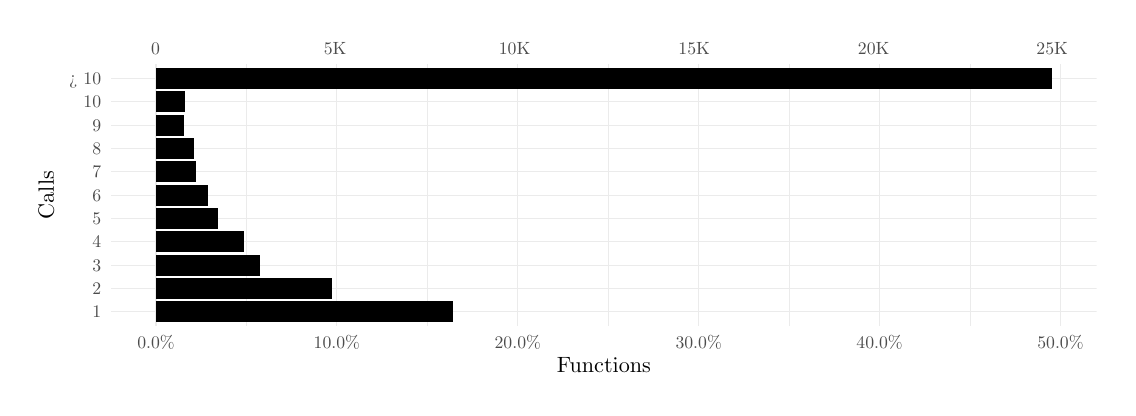
\begin{tikzpicture}[x=1pt,y=1pt]
\definecolor{fillColor}{RGB}{255,255,255}
\path[use as bounding box,fill=fillColor,fill opacity=0.00] (0,0) rectangle (390.26,130.09);
\begin{scope}
\path[clip] ( 30.17, 22.32) rectangle (386.26,116.83);
\definecolor{drawColor}{gray}{0.92}

\path[draw=drawColor,line width= 0.2pt,line join=round] ( 79.04, 22.32) --
	( 79.04,116.83);

\path[draw=drawColor,line width= 0.2pt,line join=round] (144.41, 22.32) --
	(144.41,116.83);

\path[draw=drawColor,line width= 0.2pt,line join=round] (209.77, 22.32) --
	(209.77,116.83);

\path[draw=drawColor,line width= 0.2pt,line join=round] (275.14, 22.32) --
	(275.14,116.83);

\path[draw=drawColor,line width= 0.2pt,line join=round] (340.51, 22.32) --
	(340.51,116.83);

\path[draw=drawColor,line width= 0.4pt,line join=round] ( 30.17, 27.38) --
	(386.26, 27.38);

\path[draw=drawColor,line width= 0.4pt,line join=round] ( 30.17, 35.82) --
	(386.26, 35.82);

\path[draw=drawColor,line width= 0.4pt,line join=round] ( 30.17, 44.26) --
	(386.26, 44.26);

\path[draw=drawColor,line width= 0.4pt,line join=round] ( 30.17, 52.70) --
	(386.26, 52.70);

\path[draw=drawColor,line width= 0.4pt,line join=round] ( 30.17, 61.14) --
	(386.26, 61.14);

\path[draw=drawColor,line width= 0.4pt,line join=round] ( 30.17, 69.58) --
	(386.26, 69.58);

\path[draw=drawColor,line width= 0.4pt,line join=round] ( 30.17, 78.01) --
	(386.26, 78.01);

\path[draw=drawColor,line width= 0.4pt,line join=round] ( 30.17, 86.45) --
	(386.26, 86.45);

\path[draw=drawColor,line width= 0.4pt,line join=round] ( 30.17, 94.89) --
	(386.26, 94.89);

\path[draw=drawColor,line width= 0.4pt,line join=round] ( 30.17,103.33) --
	(386.26,103.33);

\path[draw=drawColor,line width= 0.4pt,line join=round] ( 30.17,111.77) --
	(386.26,111.77);

\path[draw=drawColor,line width= 0.4pt,line join=round] ( 46.36, 22.32) --
	( 46.36,116.83);

\path[draw=drawColor,line width= 0.4pt,line join=round] (111.72, 22.32) --
	(111.72,116.83);

\path[draw=drawColor,line width= 0.4pt,line join=round] (177.09, 22.32) --
	(177.09,116.83);

\path[draw=drawColor,line width= 0.4pt,line join=round] (242.46, 22.32) --
	(242.46,116.83);

\path[draw=drawColor,line width= 0.4pt,line join=round] (307.82, 22.32) --
	(307.82,116.83);

\path[draw=drawColor,line width= 0.4pt,line join=round] (373.19, 22.32) --
	(373.19,116.83);
\definecolor{fillColor}{RGB}{0,0,0}

\path[fill=fillColor] ( 46.36,107.97) rectangle (370.07,115.57);

\path[fill=fillColor] ( 46.36, 23.58) rectangle (153.52, 31.18);

\path[fill=fillColor] ( 46.36, 99.53) rectangle ( 56.78,107.13);

\path[fill=fillColor] ( 46.36, 32.02) rectangle (109.88, 39.62);

\path[fill=fillColor] ( 46.36, 40.46) rectangle ( 83.98, 48.06);

\path[fill=fillColor] ( 46.36, 48.90) rectangle ( 78.12, 56.49);

\path[fill=fillColor] ( 46.36, 57.34) rectangle ( 68.81, 64.93);

\path[fill=fillColor] ( 46.36, 65.78) rectangle ( 65.03, 73.37);

\path[fill=fillColor] ( 46.36, 74.22) rectangle ( 60.74, 81.81);

\path[fill=fillColor] ( 46.36, 82.66) rectangle ( 60.20, 90.25);

\path[fill=fillColor] ( 46.36, 91.10) rectangle ( 56.47, 98.69);
\end{scope}
\begin{scope}
\path[clip] (  0.00,  0.00) rectangle (390.26,130.09);
\definecolor{drawColor}{gray}{0.30}

\node[text=drawColor,anchor=base,inner sep=0pt, outer sep=0pt, scale=  0.64] at ( 46.21,120.43) {0};

\node[text=drawColor,anchor=base,inner sep=0pt, outer sep=0pt, scale=  0.64] at (111.09,120.43) {5K};

\node[text=drawColor,anchor=base,inner sep=0pt, outer sep=0pt, scale=  0.64] at (175.96,120.43) {10K};

\node[text=drawColor,anchor=base,inner sep=0pt, outer sep=0pt, scale=  0.64] at (240.83,120.43) {15K};

\node[text=drawColor,anchor=base,inner sep=0pt, outer sep=0pt, scale=  0.64] at (305.70,120.43) {20K};

\node[text=drawColor,anchor=base,inner sep=0pt, outer sep=0pt, scale=  0.64] at (370.22,120.43) {25K};
\end{scope}
\begin{scope}
\path[clip] (  0.00,  0.00) rectangle (390.26,130.09);
\definecolor{drawColor}{gray}{0.30}

\node[text=drawColor,anchor=base east,inner sep=0pt, outer sep=0pt, scale=  0.64] at ( 26.57, 25.18) {1};

\node[text=drawColor,anchor=base east,inner sep=0pt, outer sep=0pt, scale=  0.64] at ( 26.57, 33.62) {2};

\node[text=drawColor,anchor=base east,inner sep=0pt, outer sep=0pt, scale=  0.64] at ( 26.57, 42.05) {3};

\node[text=drawColor,anchor=base east,inner sep=0pt, outer sep=0pt, scale=  0.64] at ( 26.57, 50.49) {4};

\node[text=drawColor,anchor=base east,inner sep=0pt, outer sep=0pt, scale=  0.64] at ( 26.57, 58.93) {5};

\node[text=drawColor,anchor=base east,inner sep=0pt, outer sep=0pt, scale=  0.64] at ( 26.57, 67.37) {6};

\node[text=drawColor,anchor=base east,inner sep=0pt, outer sep=0pt, scale=  0.64] at ( 26.57, 75.81) {7};

\node[text=drawColor,anchor=base east,inner sep=0pt, outer sep=0pt, scale=  0.64] at ( 26.57, 84.25) {8};

\node[text=drawColor,anchor=base east,inner sep=0pt, outer sep=0pt, scale=  0.64] at ( 26.57, 92.69) {9};

\node[text=drawColor,anchor=base east,inner sep=0pt, outer sep=0pt, scale=  0.64] at ( 26.57,101.13) {10};

\node[text=drawColor,anchor=base east,inner sep=0pt, outer sep=0pt, scale=  0.64] at ( 26.57,109.57) {> 10};
\end{scope}
\begin{scope}
\path[clip] (  0.00,  0.00) rectangle (390.26,130.09);
\definecolor{drawColor}{gray}{0.30}

\node[text=drawColor,anchor=base,inner sep=0pt, outer sep=0pt, scale=  0.64] at ( 46.36, 14.31) {0.0{\%}};

\node[text=drawColor,anchor=base,inner sep=0pt, outer sep=0pt, scale=  0.64] at (111.72, 14.31) {10.0{\%}};

\node[text=drawColor,anchor=base,inner sep=0pt, outer sep=0pt, scale=  0.64] at (177.09, 14.31) {20.0{\%}};

\node[text=drawColor,anchor=base,inner sep=0pt, outer sep=0pt, scale=  0.64] at (242.46, 14.31) {30.0{\%}};

\node[text=drawColor,anchor=base,inner sep=0pt, outer sep=0pt, scale=  0.64] at (307.82, 14.31) {40.0{\%}};

\node[text=drawColor,anchor=base,inner sep=0pt, outer sep=0pt, scale=  0.64] at (373.19, 14.31) {50.0{\%}};
\end{scope}
\begin{scope}
\path[clip] (  0.00,  0.00) rectangle (390.26,130.09);
\definecolor{drawColor}{RGB}{0,0,0}

\node[text=drawColor,anchor=base,inner sep=0pt, outer sep=0pt, scale=  0.80] at (208.22,  5.56) {Functions};
\end{scope}
\begin{scope}
\path[clip] (  0.00,  0.00) rectangle (390.26,130.09);
\definecolor{drawColor}{RGB}{0,0,0}

\node[text=drawColor,rotate= 90.00,anchor=base,inner sep=0pt, outer sep=0pt, scale=  0.80] at (  9.51, 69.58) {Calls};
\end{scope}
\end{tikzpicture}

  \caption{Call Distribution}
  \label{fig:callDist}
\end{figure}
%
We observe 294.45M arguments created in our execution traces. Of those 3.9M are
missing, 18.9M are $...$ arguments, and 271.6M are promises. These arguments
correspond to 185.9K parameter positions of the 50,435 functions for which we
generate signatures. Figure ~\ref{fig:paramDist} shows the distribution of these
parameters per function.
%
\begin{figure}[!h]
  \centering
  % Created by tikzDevice version 0.12.3.1 on 2021-04-09 22:35:57
% !TEX encoding = UTF-8 Unicode
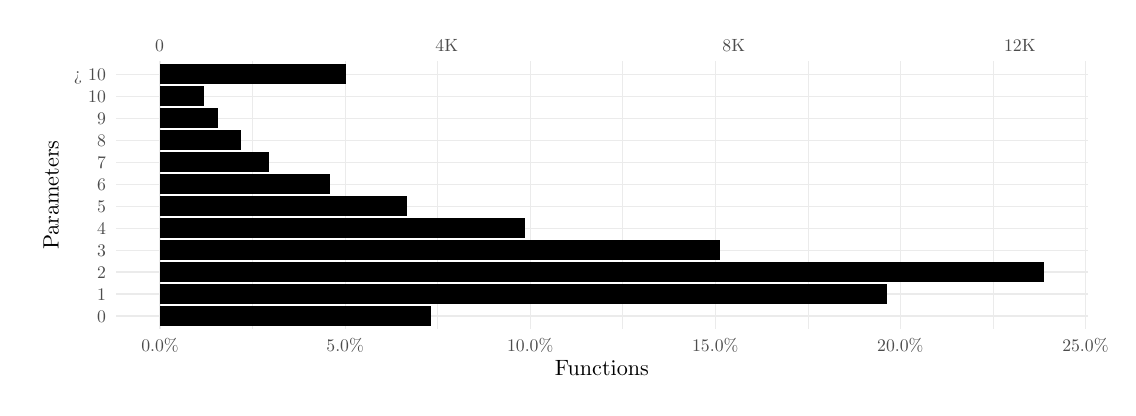
\begin{tikzpicture}[x=1pt,y=1pt]
\definecolor{fillColor}{RGB}{255,255,255}
\path[use as bounding box,fill=fillColor,fill opacity=0.00] (0,0) rectangle (390.26,130.09);
\begin{scope}
\path[clip] ( 31.86, 21.16) rectangle (383.14,117.99);
\definecolor{drawColor}{gray}{0.92}

\path[draw=drawColor,line width= 0.2pt,line join=round] ( 81.27, 21.16) --
	( 81.27,117.99);

\path[draw=drawColor,line width= 0.2pt,line join=round] (148.15, 21.16) --
	(148.15,117.99);

\path[draw=drawColor,line width= 0.2pt,line join=round] (215.02, 21.16) --
	(215.02,117.99);

\path[draw=drawColor,line width= 0.2pt,line join=round] (281.90, 21.16) --
	(281.90,117.99);

\path[draw=drawColor,line width= 0.2pt,line join=round] (348.77, 21.16) --
	(348.77,117.99);

\path[draw=drawColor,line width= 0.4pt,line join=round] ( 31.86, 25.92) --
	(383.14, 25.92);

\path[draw=drawColor,line width= 0.4pt,line join=round] ( 31.86, 33.86) --
	(383.14, 33.86);

\path[draw=drawColor,line width= 0.4pt,line join=round] ( 31.86, 41.80) --
	(383.14, 41.80);

\path[draw=drawColor,line width= 0.4pt,line join=round] ( 31.86, 49.73) --
	(383.14, 49.73);

\path[draw=drawColor,line width= 0.4pt,line join=round] ( 31.86, 57.67) --
	(383.14, 57.67);

\path[draw=drawColor,line width= 0.4pt,line join=round] ( 31.86, 65.61) --
	(383.14, 65.61);

\path[draw=drawColor,line width= 0.4pt,line join=round] ( 31.86, 73.54) --
	(383.14, 73.54);

\path[draw=drawColor,line width= 0.4pt,line join=round] ( 31.86, 81.48) --
	(383.14, 81.48);

\path[draw=drawColor,line width= 0.4pt,line join=round] ( 31.86, 89.42) --
	(383.14, 89.42);

\path[draw=drawColor,line width= 0.4pt,line join=round] ( 31.86, 97.35) --
	(383.14, 97.35);

\path[draw=drawColor,line width= 0.4pt,line join=round] ( 31.86,105.29) --
	(383.14,105.29);

\path[draw=drawColor,line width= 0.4pt,line join=round] ( 31.86,113.23) --
	(383.14,113.23);

\path[draw=drawColor,line width= 0.4pt,line join=round] ( 47.83, 21.16) --
	( 47.83,117.99);

\path[draw=drawColor,line width= 0.4pt,line join=round] (114.71, 21.16) --
	(114.71,117.99);

\path[draw=drawColor,line width= 0.4pt,line join=round] (181.58, 21.16) --
	(181.58,117.99);

\path[draw=drawColor,line width= 0.4pt,line join=round] (248.46, 21.16) --
	(248.46,117.99);

\path[draw=drawColor,line width= 0.4pt,line join=round] (315.34, 21.16) --
	(315.34,117.99);

\path[draw=drawColor,line width= 0.4pt,line join=round] (382.21, 21.16) --
	(382.21,117.99);
\definecolor{fillColor}{RGB}{0,0,0}

\path[fill=fillColor] ( 47.83,109.66) rectangle (115.04,116.80);

\path[fill=fillColor] ( 47.83, 22.35) rectangle (145.68, 29.50);

\path[fill=fillColor] ( 47.83, 30.29) rectangle (310.59, 37.43);

\path[fill=fillColor] ( 47.83,101.72) rectangle ( 63.63,108.86);

\path[fill=fillColor] ( 47.83, 38.23) rectangle (367.18, 45.37);

\path[fill=fillColor] ( 47.83, 46.16) rectangle (250.08, 53.31);

\path[fill=fillColor] ( 47.83, 54.10) rectangle (179.66, 61.24);

\path[fill=fillColor] ( 47.83, 62.04) rectangle (137.11, 69.18);

\path[fill=fillColor] ( 47.83, 69.97) rectangle (109.42, 77.12);

\path[fill=fillColor] ( 47.83, 77.91) rectangle ( 87.10, 85.05);

\path[fill=fillColor] ( 47.83, 85.85) rectangle ( 77.25, 92.99);

\path[fill=fillColor] ( 47.83, 93.78) rectangle ( 68.76,100.93);
\end{scope}
\begin{scope}
\path[clip] (  0.00,  0.00) rectangle (390.26,130.09);
\definecolor{drawColor}{gray}{0.30}

\node[text=drawColor,anchor=base,inner sep=0pt, outer sep=0pt, scale=  0.64] at ( 47.69,121.59) {0};

\node[text=drawColor,anchor=base,inner sep=0pt, outer sep=0pt, scale=  0.64] at (151.42,121.59) {4K};

\node[text=drawColor,anchor=base,inner sep=0pt, outer sep=0pt, scale=  0.64] at (255.15,121.59) {8K};

\node[text=drawColor,anchor=base,inner sep=0pt, outer sep=0pt, scale=  0.64] at (358.53,121.59) {12K};
\end{scope}
\begin{scope}
\path[clip] (  0.00,  0.00) rectangle (390.26,130.09);
\definecolor{drawColor}{gray}{0.30}

\node[text=drawColor,anchor=base east,inner sep=0pt, outer sep=0pt, scale=  0.64] at ( 28.26, 23.72) {0};

\node[text=drawColor,anchor=base east,inner sep=0pt, outer sep=0pt, scale=  0.64] at ( 28.26, 31.66) {1};

\node[text=drawColor,anchor=base east,inner sep=0pt, outer sep=0pt, scale=  0.64] at ( 28.26, 39.59) {2};

\node[text=drawColor,anchor=base east,inner sep=0pt, outer sep=0pt, scale=  0.64] at ( 28.26, 47.53) {3};

\node[text=drawColor,anchor=base east,inner sep=0pt, outer sep=0pt, scale=  0.64] at ( 28.26, 55.47) {4};

\node[text=drawColor,anchor=base east,inner sep=0pt, outer sep=0pt, scale=  0.64] at ( 28.26, 63.40) {5};

\node[text=drawColor,anchor=base east,inner sep=0pt, outer sep=0pt, scale=  0.64] at ( 28.26, 71.34) {6};

\node[text=drawColor,anchor=base east,inner sep=0pt, outer sep=0pt, scale=  0.64] at ( 28.26, 79.28) {7};

\node[text=drawColor,anchor=base east,inner sep=0pt, outer sep=0pt, scale=  0.64] at ( 28.26, 87.21) {8};

\node[text=drawColor,anchor=base east,inner sep=0pt, outer sep=0pt, scale=  0.64] at ( 28.26, 95.15) {9};

\node[text=drawColor,anchor=base east,inner sep=0pt, outer sep=0pt, scale=  0.64] at ( 28.26,103.09) {10};

\node[text=drawColor,anchor=base east,inner sep=0pt, outer sep=0pt, scale=  0.64] at ( 28.26,111.02) {> 10};
\end{scope}
\begin{scope}
\path[clip] (  0.00,  0.00) rectangle (390.26,130.09);
\definecolor{drawColor}{gray}{0.30}

\node[text=drawColor,anchor=base,inner sep=0pt, outer sep=0pt, scale=  0.64] at ( 47.83, 13.15) {0.0{\%}};

\node[text=drawColor,anchor=base,inner sep=0pt, outer sep=0pt, scale=  0.64] at (114.71, 13.15) {5.0{\%}};

\node[text=drawColor,anchor=base,inner sep=0pt, outer sep=0pt, scale=  0.64] at (181.58, 13.15) {10.0{\%}};

\node[text=drawColor,anchor=base,inner sep=0pt, outer sep=0pt, scale=  0.64] at (248.46, 13.15) {15.0{\%}};

\node[text=drawColor,anchor=base,inner sep=0pt, outer sep=0pt, scale=  0.64] at (315.34, 13.15) {20.0{\%}};

\node[text=drawColor,anchor=base,inner sep=0pt, outer sep=0pt, scale=  0.64] at (382.21, 13.15) {25.0{\%}};
\end{scope}
\begin{scope}
\path[clip] (  0.00,  0.00) rectangle (390.26,130.09);
\definecolor{drawColor}{RGB}{0,0,0}

\node[text=drawColor,anchor=base,inner sep=0pt, outer sep=0pt, scale=  0.80] at (207.50,  4.40) {Functions};
\end{scope}
\begin{scope}
\path[clip] (  0.00,  0.00) rectangle (390.26,130.09);
\definecolor{drawColor}{RGB}{0,0,0}

\node[text=drawColor,rotate= 90.00,anchor=base,inner sep=0pt, outer sep=0pt, scale=  0.80] at ( 11.20, 69.58) {Parameters};
\end{scope}
\end{tikzpicture}

  \caption{Parameter Distribution}
  \label{fig:paramDist}
\end{figure}
%
7.3\% functions have 0 parameters, 19.6\% have 1, and 5.0\% have over 10. There
are 15 functions with over 50 parameters that come from 10 packages. Of those,
\c{rpart.plot::check.if.dot.arg.supported.by.rpart.rules} has the highest, 122
parameters.

%\c{ComplexHeatmap::pheatmap} (51), \c{network::plot.network.default}
%(52), \c{rpart.plot::get.layout} (53), \c{sna::gplot} (54),
%\c{Hmisc::latex.default} (55), \c{VennDiagram::draw.quintuple.venn} (57)
%\c{pROC::plot.roc.roc} (58), \c{rpart.plot::draw.node.numbers} (60),
%\c{gplots::heatmap.2} (63), \c{Hmisc::event.chart} (66),
%\c{ComplexHeatmap::Heatmap} (83), \c{ggplot2::theme} (95),
%\c{ergm::control.ergm} (117), \c{rpart.plot::prp} (119), and

Table~\ref{table:strictdist} presents a summary of the lazy arguments of the
signatures in terms of a distribution of parameters, functions, and packages
that correspond to unevaluated, effectful or reflective arguments. Row \#0 (with
tick-mark against \emph{Unevaluated}) tells that there are 128.3K parameters
from 44.4K functions whose arguments are evaluated across all calls and they
don't perform any effect or reflective operation. Similarly, row \#7 tells us
that 25 parameters from 24 functions are not evaluated in at least one call, but
whey they are evaluated, they perform a side-effect and a reflective operation.
Similarly, row \#4 tells us that 27.1K parameters from 11.3K functions are never
evaluated. A careful study of these rows yields the following insights. First,
arguments passed to majority of parameters, 65.25\%, are always evaluated and
don't perform any side-effects or reflective operations. So, they can be made
unconditionally strict . Of the remaining parameters, only unevaluated arguments
correspond to 13.76\% parameters, followed by only side-effecting arguments to
4\% parameters, and only reflective promises to 0.07\% parameters. The remaining
combinations amount to less than a percent each. It is important to note that a
function can appear in multiple rows as different parameters can belong to
different categories. Same reasoning applies to packages. Another interesting
pattern in the data is that arguments performing reflective operations
(alternate rows \#1, \#3, \#5, \#7) come from relatively few functions and
packages.
%
\begin{table}
  \vspace{-3mm}
  \small
  \caption{Signature Summary} \label{table:strictdist}
  \centering
  \begin{tabular}{lcccr|lr|lr}
    \toprule
    \#&\bf Unevaluted (U) & \bf Side-Effecting (S) & \bf Reflective (R) & \multicolumn{2}{c}{\textbf{Parameters}} & \multicolumn{2}{c}{\textbf{Functions}}& \bf Packages\\
    \midrule
    0&\xmark{}&\xmark{}&\xmark{}&128305&65.25\%&44377&85.93\%&489\\
    1&\xmark{}&\xmark{}&\cmark{}&134&0.07\%&124&0.24\%&47\\
    2&\xmark{}&\cmark{}&\xmark{}&7871&4\%&5805&11.24\%&399\\
    3&\xmark{}&\cmark{}&\cmark{}&408&0.21\%&385&0.75\%&93\\
    4&\cmark{}&\xmark{}&\xmark{}&27050&13.76\%&11333&21.95\%&453\\
    5&\cmark{}&\xmark{}&\cmark{}&13&0.01\%&12&0.02\%&11\\
    6&\cmark{}&\cmark{}&\xmark{}&1213&0.62\%&813&1.57\%&199\\
    7&\cmark{}&\cmark{}&\cmark{}&25&0.01\%&24&0.05\%&15\\
    \bottomrule
  \end{tabular}
\end{table}
%
An important detail in this summary is that includes contribution of
side-effects and reflective operations performed by R's \emph{base} package and
other user packages not part of our corpus. This is because arguments are also
transitively involved in side-effecting or reflective operations. The numbers
provided in this table are upper-bounds, we over count the number of arguments
transitively involved in effects and reflective operations.

\subsection{Robustness} \label{Evaluation:Robustness}

\begin{wraptable}{r}{6cm}
  \vspace{-3mm}
  \small
  \centering
  \caption{Client Corpus}\label{table:clientcorpus}
  \vspace{-3mm}
  \begin{tabular}{lrrr}
    \toprule
    &\bf Tests&\bf Examples&\bf Vignettes\\
    \midrule
    {Scripts} &9.8K&41.1K&1.7K\\
    \midrule
    {LOC} &751.2K&348.8K&112.3K\\
    \bottomrule
  \end{tabular}
\end{wraptable}%%


For assessing the robustness of the strictness signatures, we run client
programs to exercise the functions with signatures. For client programs, we have
selected 2000 dependent packages of the 500 packages from the synthesis corpus.
They have 4.5M lines of R code and 4.7M lines of native (C, C++, and Fortran)
code. We run their examples, tests, and vignettes and measure the number of
programs that break due to the strictness signatures. Table
~\ref{table:clientcorpus} gives the number of scripts of each kind that were run
and lines of code exercised.



\AG{add evaluation orders and contrast with side effects to assess impact.}
%%the function and choose the definition order.
%%Figure~\ref{fig:force_order} shows the number of evaluation orders of the
%%functions in our corpus. XX(XX\%) functions have a single evaluation order. Out
%%of those, XX functions evaluate all of their arguments. Evaluation orders
%%greater than 5 are rare and are found only in XX functions.

% TODO for end
% Table~\cite{tab:ten_sigs} shows ten representative signatures generated by the
% synthesis step of our experiments.
%
% \begin{table}
%   \vspace{-3mm}
%   \caption{Strictness Signatures} \label{table:ten_sigs}
%   \centering
%   \begin{tabular}{ll}
%     \toprule
%     \bf Function &\bf Strictness Signature\\
%     \hline
%     \bottomrule
%   \end{tabular}
% \end{table}

\begin{table}
  \small
  \caption{Strictness Failure} \label{table:strictfail}
  \centering
  \begin{tabular}{lc|rl|rl|rl|rl|rl}
    \toprule
    \#&\textbf{Configuration}&\multicolumn{2}{c}{\textbf{test}}&\multicolumn{2}{c}{\textbf{vignette}}&\multicolumn{2}{c}{\textbf{example}}&\multicolumn{2}{c}{\textbf{testthat}}&\multicolumn{2}{c}{\textbf{total}}\\
    \midrule
    0&$+U+S+R$&5&2.09\%&25&10.46\%&163&68.2\%&46&19.25\%&239&0.56\%\\
    1&$+U+S-R$&4&1.71\%&24&10.26\%&162&69.23\%&44&18.8\%&234&0.55\%\\
    2&$+U-S+R$&28&1.46\%&101&5.25\%&1594&82.93\%&199&10.35\%&1922&4.51\%\\
    3&$+U-S-R$&41&0.62\%&99&1.49\%&1649&24.89\%&4836&73\%&6625&15.54\%\\
    4&$-U+S+R$&21&3.44\%&87&14.26\%&409&67.05\%&93&15.25\%&610&1.43\%\\
    5&$-U+S-R$&20&3.25\%&91&14.77\%&412&66.88\%&93&15.1\%&616&1.44\%\\
    6&$-U-S+R$&46&1.98\%&156&6.73\%&1861&80.25\%&256&11.04\%&2319&5.44\%\\
    7&$-U-S-R$&57&0.8\%&181&2.53\%&2084&29.11\%&4836&67.56\%&7158&16.79\%\\
    \bottomrule
  \end{tabular}
\end{table}

First, we run the client scripts twice without any signatures to filter programs
which finish successfully with the same output in both runs. This provides us
with baseline deterministic programs against which we can compare the
effectiveness of our signatures.Then, we run these programs eight times, once
for each signature configuration, and count the number of programs that fail or
produce a different output compared to the baseline output.

We rely on the output of programs for measuring correctness, \emph{i.e.}, we
believe that programs that produce the same output with and without signatures
produce the same result. Our rationale is that the top-level expressions in R
scripts print their result on the console unless it is stored in a variable or
explicitly silenced by surrounding the expressions in a call to the
\code{invisible} function. R also prints messages on library loading, function
shadowing, warnings, and errors. A simple heuristic to test our belief is to
check for the degree of duplication in programs' output. If the outputs are
unique they can be used as a ``fingerprint'' for the programs and a change in
the programs' result by applying strictness signatures will likely change the
output. This will be then be counted as a failure for that signature
configuration.

We extracted XXXX client programs of which XXXX programs were deterministic. Of
these deterministic programs, only XXXX produced the same output. The results of
applying signatures to the deterministic programs are summarized in
Table~\ref{table:strictfail}. Each row represents a signature configuration. For
each configuration we report the number and percentage of failing programs,
further broken down into failures per script type. The letters \emph{U},
\emph{S}, and \emph{R} represent unevaluated, side-effecting and reflective
arguments. The \emph{+} sign signifies that the corresponding arguments are
treated lazy in the signature configuration and \emph{-} sign means they are
evaluated eagerly. For example, $+U+E+R$ means that arguments that are
unevaluated, side-effecting, and reflective are treated lazy whereas $-U-E-R$
means that these arguments are evaluated strictly. Each row of this table
directly corresponds to a row of Table~\ref{table:strictdist}. For example,
from row \#1 of both tables, we can say the \config{1} will evaluate 134
arguments strictly.

Now, we take a deeper look at Table~\ref{table:strictfail} for insights.
\cconfig{0} corresponds to the configuration with maximum laziness and it failure rate
is only 0.56\%. We can use this as a baseline to study the impact of making
various arguments categories strict.

First, we look at the impact of making a single argument category strict. In
\config{1} only reflective arguments are made strict and surprisingly, it leads
to a slightly better result of 0.55\% failures compared to \config{0}. This
difference is however marginal. \cconfig{2} shows that evaluating only
side-effecting arguments leads to a failure rate of 4.51\%. From \config{4},
we see that evaluating unevaluated arguments leads to 1.43\% failures. Comparing
these results with the number of lazy parameters from
Table~\ref{table:strictdist}, we find that unevaluated arguments, which are the
biggest source of laziness, do not cause a significant increase in failures when
evaluated.

Next, we look at the impact of making two argument categories strict.
\cconfig{3} stands out with a very high failure rate of 15.54\%. This is
followed by \config{6} with a failure rate of 5.44\% and finally \config{5} with
a failure rate of 1.44\%. The failure rate is lowest when side-effecting
arguments are made lazy. This is validated by the low failure rate observed when
only unevaluated or reflective arguments are evaluated eagerly in \config{1} and
\config{4}.

Finally, we look at the impact of making everything strict. This corresponds to
\config{7}. As expected, this leads to maximum failure, 16.79\%. It is
interesting to compare this against \config{3}. The difference in failures for
these two configurations is marginal, suggesting that treating unevaluated
arguments strictly is not the major cause of failures. This is also validated by
\config{4} in which only unevaluted arguments are forced and failure rate is
1.43\%.


The argument evaluation orders observed for a function depend on its
implementation and the control-flow paths exercised by its inputs. In this work
we ignore this evaluation order. For evaluation robustness, we choose the
definition order in the synthesized signatures. For assessing performance, the
\Rsh just-in-time compiler uses the call order, i.e., the order in which
arguments are passed to the function at the call site.


\AG{Threats to validity: rlang has defiintion of SEXP.}


\subsection{In-Depth Exploration}\label{sec:lazr-discussion}

In this section, we present a quantitative and qualitative discussion of the
different sources of laziness.

\subsubsection{Metaprogramming}

\begin{wraptable}{r}{4cm}
  \vspace{-3mm}
  \small
  \caption{Metaprogramming} \label{table:meta}
  \centering
  \begin{tabular}{lll}
    \toprule
    &\textbf{C}&\textbf{R}\\
    \midrule
    Arguments&21.9M&1.3M\\
    Parameters&9.1K&600\\
    Functions&6.0K&370\\
    Packages&374&89\\
    \bottomrule
  \end{tabular}
\end{wraptable}

For capturing uses of metaprogramming, we track calls to \code{substitute} on
function arguments from R code and \code{PREXPR} macro on promise objects from C
code. The results are summarized in Table~\ref{table:meta}. There are two
interesting observations to make from this table. First, metaprogramming is not
very common, only 23.2M out of 294.25 total arguments are metaprogrammed.
Second, metaprogramming is dominated by the use of \code{PREXPR} macro on
promise objects from C code.

For an in-depth discussion on the patterns of use of \code{substitute}, we refer
the reader to \citet{oopsla19b}. We continue with the exploration of the use of
\code{PREXPR} for metaprogramming, since that is not addressed in
\cite{oopsla19b}. The maximum uses of \code{PREXPR} come from the builtin
functions.
A canonical example is the \code{missing} function for checking if an
argument is missing. Missingness check works transitively, since it is possible
to pass missing arguments to callees. The \code{missing} function first checks
if the argument is bound to a sentinel missing value. If not, it checks if the
argument is bound to a promise containing a symbol. This symbol is then checked
in the caller's environment for missingness.

Apart from this, many packages implement functionality in native code and use
\code{PREXPR} to extract a promise's expression for ad-hoc evaluation
strategies. We found uses of \code{PREXPR} in \code{igraph}, \code{lazyeval},
\code{rlang} and \code{S4Vectors} packages of our corpus. \code{rlang}
particularly stands out because it provides an API to work with core R objects,
including a rich set of APIs for metaprogramming. It frequently calls into C
code for heavy lifting.

\subsubsection{Unevaluated Arguments}
Of the 294.45M total arguments in our corpus, 30.4M argument promises were not
evaluated. They correspond to 52,083 parameters of 26,398 functions from 473
packages. These functions are non-strict in the corresponding parameters.
%
Based on argument evaluation, we can classify parameter positions into three
categories.\always parameters are those whose arguments are evaluated in all
calls. \sometimes parameters are those whose arguments are evaluated at least
once but not always. \never parameters are those whose arguments are never
evaluated. Table~\ref{table:argeval} shows the number and proportion of
parameters that belong to these categories.

\begin{table}[!h]
  \vspace{-3mm}
  \caption{Argument Evaluation}\label{table:argeval}
  \vspace{-3mm}
  \begin{tabular}{lr|lr|lr}
    \toprule
    \textbf{Type}&\multicolumn{2}{c}{\textbf{Parameters}}&\multicolumn{2}{c}{\textbf{Functions}}&\textbf{Packages}\\
    \midrule
    Always&144565&73.51\%&48456&96.08\%&490\\
    Sometimes&16411&8.35\%&7070&14.02\%&410\\
    Never&10637&5.41\%&5907&11.71\%&405\\
    \midrule
    Sometimes*&15130&7.69\%&6609&13.1\%&406\\
    Never*&9251&4.7\%&5121&10.15\%&400\\
    \bottomrule
  \end{tabular}
\end{table}

Majority of parameters are \always parameters, suggesting that arguments passed
to functions are evaluated in most of the cases. This is followed by 8.35\%
\sometimes parameters. Their presence indicates use of metaprogramming or
unexplored control flow paths in the function. Lastly, we have 5.41\% \never
arguments whose presence indicates lack of coverage, metaprogramming, or dummy
parameter. The \textbf{Functions} field gives the number of functions with
\always, \sometimes, and \never arguments. The same function can appear in
multiple columns since different parameters can have different evaluation
classification. The \textbf{Packages} field of Table~\ref{table:areval} tells us
that \never and \sometimes functions are spread across many packages.
%
\sometimesStar and \neverStar in Table~\ref{table:argeval} are the number of
\sometimes and \never cases without metaprogrammed. The different is small which
suggests that metaprogramming is not the primary reason for arguments remaining
unevaluated. Turning to the number of calls, we find that 78.33\% of functions
with \never parameters are called more than once. This suggests that a lack of
call diversity could be one of factors for \never arguments' existence. With
better call diversity, the \never parameters will turn into \sometimes.

\paragraph{Qualitative Analysis}

We analyzed a sample of functions with \sometimes and \never parameters to
identify usage patterns.
%
First, we look at \sometimes parameters. A common patter occurring in 30
packages is the following definition of \code{\%||\%} function.
%
\begin{lstlisting}
lazyeval::\%||\% <- function(x, y) if(is.null(x)) y else x
\end{lstlisting}
%
This function evaluates its second argument \code{y} only if \code{x} is
\code{NULL}. This makes \code{y} a \sometimes parameter. This pattern suggests
that \code{y} is a \sometimes parameter for a reason and should not be evaluated
unless needed. However, there are other functions with multiple paths where
evaluating the \sometimes argument is expected to be benign. For example, in
\code{bayesplot::is_whole_number} function, the \code{tol} argument is only
evaluated when \code{x} is a numeric value.
%
\begin{lstlisting}
bayesplot::is_whole_number <- function(x, tol = .Machine$double.eps) {
    if (!is.numeric(x)) { FALSE } else { abs(x - round(x)) < tol }
}
\end{lstlisting}

Another pattern occurring in 4 packages is the definition of
\code{on_package_load}.

\begin{lstlisting}
glue::on_package_load <- function(pkg, expr) {
    if (isNamespaceLoaded(pkg)) { expr }
    else {
        thunk <- function(...) expr
        setHook(packageEvent(pkg, "onLoad"), thunk)
    }
}
\end{lstlisting}
%
Here, if package \code{pkg} is not loaded, the \code{expr} argument's evaluation
is delayed until the package's \code{onLoad} event occurs. In some executions,
we see the \code{expr} argument being evaluated if package \code{pkg} is loaded
and in other iterations, we don't. The way this code is written suggests that
\code{expr} should not be evaluated strictly.
%
S3 generics result in many \sometimes and \never parameters. These functions
dynamically dispatch to a specific implementation with the same name based on
the first argument's class. In this case, the first argument is always evaluated
but the remaining arguments might not be needed by the specific method. Across
all executions, we observed that \code{n} and \code{m} are evaluated sometimes
but \code{r} is never evaluated.
%
\begin{lstlisting}
abind::acorn <- function(x, n=6, m=5, r=1, ...) UseMethod('acorn')
\end{lstlisting}

Next, we turn our attention to \never parameters.
%
The most common case is when an argument is not used in some branch of the
function. Due to lack of call diversity, the branch in which the argument is
used is never taken and the parameter is classified as \never. For example,
\code{discretize} function of package \code{actuar} only uses \code{xlim} if
\code{from} and \code{to} parameters are missing.
\begin{lstlisting}
actuar:::discretize <- function (cdf, from, to, ..., xlim = NULL) {
    ...
    if (missing(from)) from <- xlim[1];
    if (missing(to)) to <- xlim[2];
    ...
}
\end{lstlisting}
%
Another pattern leading to \never parameters is when a function is called with a
certain interface even if it does not use those arguments. R calls a package's
\code{.onLoad} function with arguments \code{libname} and \code{pkgname} when
the package is loaded. The \code{.onLoad} hook of \code{assertive.base} package
ignores them.
\begin{lstlisting}
assertive.base::.onLoad <- function(libname, pkgname) {
    options(assertive.severity = "stop")
}
\end{lstlisting}
%
The \code{proxy} package defines over a dozen methods with the interface
\code{function(a, b, c, d, n) ...} that implement different proximity metrics by
using only a subset of the arguments.
This also happens in method dispatch when the generic method defines a parameter
which is not used by the specific method. For example \code{bit64} package
defines \code{unipos} generic method with a parameter \code{incomparables} which
is not used by its only concrete implementation \code{unipos.integer64}

Sometimes arguments don't need to be used by design.
The \code{tail} operation in package \code{dbplyr} is not defined for
\code{tbl_lazy} objects. So the function throws an error when called without
using any of its arguments.
\begin{lstlisting}
dbplyr::tail.tbl_lazy <- function(x, n = 6L, ...) {
    stop("tail() is not supported by sql sources", call. = FALSE)
}
\end{lstlisting}
%
Sometimes packages implement a specialized compatible wrapper.
\code{jsonlite} package implements \code{stop} function with the same interface
as R's \code{base} package's \code{stop} function but ignores its \code{call.}
argument.
\begin{lstlisting}
jsonlite::stop <- function(..., call. = FALSE) {
    base::stop(..., call. = FALSE)
}
\end{lstlisting}
%
\never parameters can also represent an erroneous condition that would not
happen in a correct program. In \code{codetools} package, function
\code{checkSymOrString} fails if the argument does not have the correct type. In
all the calls we observed, the \code{signal} argument was not used because
\code{e} had the correct type.
\begin{lstlisting}
codetools::checkSymOrString <- function(e, signal = stop) {
    type <- typeof(e)
    if (type == "symbol" || type == "character") e
    else signal("not a symbol or string")
}
\end{lstlisting}

\subsubsection{Reflection}

R allows reflective access to parent scope through \code{as.environment} and
\code{pos.to.env} functions when called with argument \code{-1}.
They return the environment of the caller with respect to call in which they are
evaluated. Consider the following example in which function f is called with the
same argument \code{as.environment(-1)} for both \code{x} and \code{y}
parameters. The first argument \code{x} is evaluated immediately inside
function \code{f} and the second argument \code{y} is evaluated inside the
\code{id} function. \code{x} evaluates to the environment of the parent of
\code{f} which is the \code{global} environment, whereas \code{y} evaluates to
the environment of \code{f} which is the parent of \code{id} inside of which
\code{y} is evaluated.
%
\begin{lstlisting}
id <- function(a) a
f <- function(x, y) { x; id(y); }
f(x = as.environment(-1), y = as.environment(-1))
\end{lstlisting}
%
There are two points to note here. First, the strictness of \code{f} with
respect to \code{x} and \code{y} depends on how \code{f} is called. Second,
\code{f} will now be lazy in argument \code{y}, otherwise we will end up
evaluating inside \code{f}. Erroneously evaluating \code{y} strictly would
result in an incorrect environment, but not an error, which could turn into a
debugging nightmare.
\code{as.environment} is internally implemented using \code{pos.to.env} so the
two functions have same semantics when called with \code{-1} as the argument.
It is interesting to note that there are other functions providing reflective
access to call stack frames such as \code{parent.frame}, \code{sys.frame}, etc.
However, these take into account the current evaluation environment to identify
the parent caller. A promise evaluates the argument expression inside the
caller's environment. So, a call to \code{parent.frame()} directly inside the
argument will use the caller's environment to identify the parent dynamic scope.
This makes its result independent of the point at which the promise is
evaluated.

Another wrinkle introduced by this setup is that it can transitively affect the
strictness of other function arguments. Imagine \code{f} is called from \code{g}
as shown below.

\begin{lstlisting}
g <- function(u, v) {
    f(u, v)
}
g(as.environment(-1), as.environment(-1))
\end{lstlisting}
%
Clearly, in this case we have to make \code{g} non-strict in \code{u} and
\code{v}. Their results depend upon how they are evaluated inside \code{f}.
%
We identified 2710 arguments which directly call \code{as.environment(-1)} and
\code{pos.to.env(-1)} in our corpus. They correspond to 2 parameters from 2
functions, \code{R.oo::.getFunctionByName}, and \code{backports:::get0}.
%
\code{R.oo:::.getFunctionByName} is a private function of \code{R.oo} package
which searches for a function by name in different scopes, configured by its
arguments. Its fourth parameter, \code{callEnvir}, has a default value of
\code{as.environment(-1)}. It is called 2707 times. The relevant part of its
definition is that \code{callEnvir} is evaluated by assigning it to
\code{envirT} before it is passed down to the \code{exists} function.
%
\begin{lstlisting}
function(name, where = c("ns", "search", "ns*"),
         envir = NULL, callEnvir = as.environment(-1L),
         class = "function", mustExist = TRUE, ...) {
    ...
    envirT <- callEnvir
    if (exists(name, mode = "function", envir = envirT, inherits = TRUE))
    ...
}
\end{lstlisting}
%
\code{backports::get0} is a private function of \code{backports} package which
looks up a variable in a scope, similar in spirit to
\code{R.oo:::.getFunctionByName}. This function is called 3 times, always with
the default value \code{pos.to.env(-1)} for \code{envir} argument. Unlike
\code{R.oo:::.getFunctionByName}, \code{backports:::get0} passes \code{envir}
unevaluated to \code{mget}. \code{mget} in turn evaluates \code{envir} and looks
up variable referred to by \code{x} in \code{envir}. Clearly, with the default
value of \code{envir}, lookup will happen in the environment of
\code{backports::get0} which only has bindings for its parameters. What makes
this work is that it is only called from the top-level, with the argument
\code{inherits} set to \code{TRUE}. This causes \code{mget} to search
recursively in enclosing scopes beginning from \code{envir} until lookup
succeeds in the \code{global} environment used for top-level bindings.
%
\begin{lstlisting}
function (x, envir = pos.to.env(-1L), mode = "any",
          inherits = TRUE, ifnotfound = NULL)  {
    ....
    mget(x[1L], envir = envir, mode = mode,
         inherits = inherits, ifnotfound = list(ifnotfound))[[1L]]
}
\end{lstlisting}
%
Calls to \code{R.oo:::.getFunctionByName} result in transitively making 1821
argument lazy. They correspond to 18 parameters from 15 functions of 3 packages.
We manually analyzed these cases but found that none of these functions pass
their arguments containing calls to \code{as.environment(-1)} or
\code{pos.to.env(-1)} to \code{R.oo:::.getFunctionByName}. They are identified
as lazy because our dynamic analyzer is conservative. When a reflective call
happens from an argument promise, it taints all the function arguments on the
stack. This has the effect of making more arguments lazy than needed.
%
\code{backports::get0} is invoked from the top-level so it does not result in
spurious transitive laziness.

\subsubsection{Side-Effects}

\begin{wraptable}{r}{5cm}
  \vspace{-3mm}
  \small
  \caption{Promise Expression} \label{table:promexpr}
  \centering
  \begin{tabular}{llllll}
    \toprule
    \textbf{Expression}&\textbf{All \%}&\textbf{SE \%}\\
    \midrule
    Symbol&48.99\%&0.11\%\\
    Value&21.58\%&0\%\\
    Call&17.49\%&0.39\%\\
    Promise&4.18\%&0\%\\
    \bottomrule
  \end{tabular}
\end{wraptable}

Arguments perform side effects when they contain a symbol, or a function call.
Occasionally, the interpreter wraps arguments inside other arguments which could
lead to transitive effects. Table ~\ref{table:promexpr} shows the distribution
of expression type inside side-effecting argument promises and contrasts it
against all argument promises. Only 0.5\% arguments perform any effect. Out of
these, 0.39\% contain a function call expression and 0.11\% contain a symbol. As
expected, arguments containing a value don't perform any effect. All promises
containing a symbol will perform at least one lookup upon evaluation. Similarly,
promises containing function calls will perform local side-effects in the
function's scope. Our algorithm is able to discard most of these ``benign''
events.

\begin{table}
  \vspace{-3mm}
  \small
  \caption{Effects} \label{table:effects}
  \centering
  \begin{tabular}{llllll}
    \toprule
    \textbf{Effect}&\textbf{Count}&\textbf{Arguments}&\textbf{Parameters}&\textbf{Functions}&\textbf{Packages}\\
    \midrule
    L&3.7M&1.2M&5.6K&3.7K&359\\
    D&1.1M&159.0K&3.0K&2.6K&319\\
    A&235.8K&122.7K&511.0&487.0&109\\
    R&2.8K&718.0&27.0&24.0&10\\
    \bottomrule
  \end{tabular}
\end{table}

Table~\ref{table:effects} shows the number of effects, lookups (L), definitions
(D), assignments (A), removals (R), and errors (E) and the number of arguments,
parameters, functions and packages that are directly responsible for those
effects. We observe that lookups are the most common cause for making arguments
lazy. This is followed by definitions and assignments. Removing bindings from
environments is not a common operation. Errors in argument positions were not
observed. Functions performing lookups, definitions and assignments are spread
across many packages.
%
Comparing the number of events in this table against the total number of events
from Table~\ref{table:events}, we find that our algorithm is able to filter
89.4B variable lookups to 3.7M, 20.9B definitions to 1.1M, 7.6B assignments to
235.8K, 360.7M removals to 2.8K, and 494 errors to 6.

\begin{table}
  \small
  \begin{minipage}{.3\linewidth}
  \centering
  \caption{Effect Sequence} \label{table:effectseq}
  \begin{tabular}{lll}
    \toprule
    \textbf{Sequence}&\textbf{Arguments}\\
    \midrule
    -&99.5\%\\
    L+&0.41\%\\
    D+&0.04\%\\
    A+&0.03\%\\
    (L+D+)+&0.01\%\\
    \bottomrule
  \end{tabular}
  \end{minipage}%
  \begin{minipage}{.6\linewidth}
  \centering
  \caption{Transitive Effects} \label{table:transeffects}
  \begin{tabular}{llll}
    \toprule
    \textbf{Effect}&\textbf{Parameters}&\textbf{Functions}&\textbf{Packages}\\
    \midrule
    L&1.4K&1.1K&230\\
    D&978&934&202\\
    A&303&298&79\\
    R&34&33&15\\
    E&6&6&3\\
    \bottomrule
  \end{tabular}
  \end{minipage}
\end{table}

An argument can perform a combination of effects during
evaluation.Table~\ref{table:effectseq} shows the sequence of operations
performed by the arguments in our corpus. Majority of arguments, 99.5\% to be
precise, do not perform any relevant effect. 0.41\% only perform a sequence of
lookups, 0.04\% perform a sequence of definitions, 0.03\% perform assignments,
and 0.01\% perform a sequence of lookups and definitions. From this, we conclude
that majority of arguments have a simple pattern of events.
%
When making side-effecting arguments lazy, we also take transitivity into
account. Unevaluated side-effecting arguments can be forwarded to callees which
will make the corresponding callee arguments lazy.
Table~\ref{table:transeffects} shows the number of parameters that are made
transitively lazy. These numbers are an upper bound. Our algorithm trades off
precision for scalability, so when a side-effect happens, it marks all the
arguments being evaluated as lazy. However, as the numbers indicate, the impact
of this imprecision is limited.

\paragraph{Qualitative Analysis}

A common source of non-local writes is the \emph{shiny} package used for
building interactive webapps in a reactive style. For example, consider the call
to \code{bindEvent} below which attaches an observer expression \code{x} to an
event \code{trigger()}. The observer expression performs a non-local side-effect
using the \code{<<-} super-assignment operator. This operator mutates in the
parent scope.
%
\begin{lstlisting}
bindEvent(trigger(), x = observe({\n    vals <<- c(vals, val())\n}))
\end{lstlisting}
%
This kind of pattern is common in applications using \emph{shiny} to update the
program state in response to events. \code{bindCache} and
\code{isolate} functions from this package are also called similarly with
side-effecting expressions.

Another important source of non-local writes is the use of functions from
\code{withr} package. It provides a set of functions to evaluate code in
temporarily modified global state. It is typical of these code blocks to compute
a value and assign it to the variable in the current scope. We observe
side-effecting expressions passed to \code{with\_dir} which temporarily changes
the current working directory, \code{with\_envvar} which changes the environment
variables, \code{with\_locale} which changes the current locale,
\code{with\_options} which changes global program options, \code{with\_par},
which changes graphical parameters for plotting, and \code{with\_seed} which
changes the random number generation seed. The listing below shows some
side-effecting calls to these functions that we observed in our corpus.
%
\begin{lstlisting}
with_envvar(c(R_ENVIRON_USER = ".Renviron"), { res <- ... })
with_dir(path_dir(wd), { base <- path_file(wd); ... })
with_seed(seed <- sample.int(.Machine$integer.max, 1), runif(5))
with_options(list(callr.cond_hndlr = function(x) cond <<- x), rs$run(do))
with_par(list(las = 1), { thm <- theme_par(); ...})
with_locale(c(LC_CTYPE = "C"), { name <- "A"; ...})
\end{lstlisting}
%
Frequently these side-effecting patterns occur in test cases written using the
\code{testthat} library where the global state is modified temporarily to test
its effect on the function under consideration.
%
A very common pattern that leads to side-effects is when the result of an
intermediate computation is assigned to a variable for subsequent use. In the
call below, the intermediate result is assigned to \code{x} before being passed
on to the \code{as.data.table} function.
%
\begin{lstlisting}
as.data.table(x <- as.character(sample(letters, 5)))
\end{lstlisting}
%
This pattern is particularly common in \emph{testthat} tests.
%
\begin{lstlisting}
expect_that(fe1 <- fixef(fm1), is_equivalent_to(1527.5))
\end{lstlisting}
%
Since our analysis is conservative, at times we mis-classify arguments when they
are not performing any visible side-effects.

Now, we discuss some examples where arguments remove a variable from a scope.
This usually happens when a function calls the \code{base} package's
\code{remove} or \code{rm} function.
%
A frequent pattern that shows up is from the \code{knitr} package. The function
\code{in_dir} evaluates a code block from an RMarkdown notebook in a specific
directory. The code block is wrapped in \code{evaluate::evaluate} function which
sets and removes handlers for intercepting abnormal conditions when evaluating
the block. The removal of a handler results in a call to the \code{remove}
function from the \code{base} package of R for removal.
%
\begin{lstlisting}
in_dir(input_dir(), evaluate(code, envir = env, ...))
\end{lstlisting}
%
The \code{evaluate} function is used quite often from many other sources. For
example, the \code{testthat::expect_snapshot} function in the \code{testthat}
testing library is used for storing a snapshot of the output of a code block for
manual inspection. It internally evaluates the code block using the
\code{evaluate} function.
%
We also observe a lot of variable removals from the \code{BiocParallel} package.
The following line of code results in a call to \code{bplapply} which performs a
parallel map operation. This function internally calls a package scope cluster
manager which removes references to clusters from an environment on cleanup
using the \code{rm} function.
%
\begin{lstlisting}
bptry(bplapply(si, FUN1, ..., BPREDO = BPREDO[idx], BPPARAM = BPPARAM))
\end{lstlisting}

Another use of \code{rm} is in the \code{[.data.table} function which is used
for subsetting a \code{data.table}. The function computes the number of rows of
the data frame and assigns to a variable \code{.N} in the caller's environment.
Eventually, it removes the variable using \code{rm}.
%
\begin{lstlisting}
[.data.table <- function (x, i, j, ...) {
    ...
    assign(".N", nrow(x), envir=parent.frame(), inherits=FALSE)
    remove.N = TRUE
    ...
    if (remove.N) rm(list=".N", envir=parent.frame())
    ...
}
\end{lstlisting}

Lastly, a very popular package, \code{rlang}, defines a function \code{env_bind}
which can be used to create and remove bindings from an environment. When passed
with the value \code{zap()}, it removes the corresponding symbol from the
environment. Instead of using \code{base} package functions, it uses the C API
function \code{R_removeVarFromFrame} exported by R to remove environment
bindings.
%
\begin{lstlisting}
env_bind(current_env(), foo = zap())
\end{lstlisting}
%
We observe 0 cases where a function's argument produces an error on evaluation.
However, we do observe 6 cases where an argument is transitively responsible for
errors. Here is a call expression which accounts for 3 of those cases.
%
\begin{lstlisting}
get_str_output(context_eval(join(src), private\$context, serialize))
\end{lstlisting}
%
Here, \code{V8::get_str_output} is called whose first argument in turn calls
\code{V8::context_eval} which in turn calls \code{V8::join}. The \code{src}
argument passed to join is bound to a promise that reads the contents from a
file. The file is missing and this raises an error. This example is interesting
because it shows how the error originates in a file reading function from
\code{base} package making three caller functions transitively responsible.

\AG{TODO: appeal to intuition for lookups since the actual examples are hard to decipher.}

\section{\Rsh: Compiling the Lazy Away}\label{sec:rsh}

In this section we report on our experiments to evaluate the implications of
eagerness on an implementations of R. To that end we modified \Rsh, a just-in-time
compiler for the language. \Rsh is based on the GNU R reference implementation
and introduces an additional two-tiered compilation strategy. The
first tier is realized by a naive bytecode interpreter, the second tier
by an optimizing native compiler. The compiler employs, among many other
optimizations, speculative inlining of R closures and promises \citep{dls19,
oopsla20c}.
The reason for choosing \Rsh as the target for our
experiments is that it allows us to better evaluate the impact of laziness. In
\Rsh we can both measure the impact on an interpreter with few optimizations
applied to the bytecode, and an optimizing compiler that already does its best
to elide promises (as long as the default semantics allows it).
To conduct our evaluation, we changed the first-tier
compiler to eagerly evaluate all arguments at all call-sites, except for a
manually curated list of exceptions. This eager bytecode also serves as the source
code for the optimizing tier. In the following we will refer
to this modified implementation as \Rshstrict.

Our main hypothesis regarding performance is that eager semantics lead to faster
execution of R programs. This hypothesis might seem unexpected to some readers,
as call-by-need is sometimes used to avoid unnecessary computation in a program.
On the other hand, delaying computations is more complex to implement and we
observed it to obstruct performance in two ways: First, it leads to more
allocations of promises used to represent the delayed computation. Second, in
combination with effects potentially originating from promises, it obstructs
more advanced compiler analysis and optimizations. Thus, we expect the hypothesis
to also hold for a just-in-time compiler that uses advanced optimizations.
In particular, we pose the following predictions:
(1) eager semantics should improve performance of most benchmarks, for both tiers
of \Rsh; (2) a significant portion of the speedup is due to reduced garbage
collection pressure; (3) and there is an additional speedup due to improved compiler
optimizations. In the following, we will present our evidence in support of (1)
and (3), and partial evidence for (2).

\paragraph{Methodology}

We evaluate the effects of our modifications on the \Rsh benchmark suite.
To ease the discussion, the results are presented on a representative subset of
the suite which includes one variant of
each benchmark. As should be no surprise given the results presented so far,
only a handful of functions, such as
\lstinline{tryCatch}, had to be kept lazy for all the benchmarks to compute
the correct results.
All of the following experiments are run on a dedicated benchmark machine, with
all background tasks disabled. The system features an Intel i7-6700K CPU, stepping 3,
microcode 0xe2 with 4 cores and 8 threads. The system has 32 GB of RAM and is
running Ubuntu 18.04 on a 4.15.0-136 Linux kernel. For ease of use, experiments
are built as containers, based on Ubuntu 20.04, and executed on
the Docker runtime 20.10.5, build 55c4c88. We verified the overhead introduced by
the containerization to be uniform. All measurements are recorded repeatedly and we
keep a historical record to spot unstable behavior. This lead us to exclude the
\lstinline{convolution} benchmark from the suite, which appears to have a
bi-modal performance profile, likely caused by the llvm backend of \Rsh.
Table~\ref{table:bms} in the appendix presents our benchmark selection.

Performance measurements are gathered by running $t_e$ invocations of \Rsh on
each benchmark. Within each invocation we measure the execution time of $t_i$
in-process invocations. For each invocation, the first 5 in-process iterations
are discarded to exclude warmup behavior. Aggregate numbers are reported as the
speedup over the arithmetic mean of the execution times. Multiple speedup
numbers are averaged using a geometric mean. To establish a baseline we measured
the speedup of \Rsh over GNU R, on our subsetted benchmark suite with parameters
$t_e = 1, t_i = 15$. We found a mean speedup of \speedupRsh, ranging between
\speedupRshMin and \speedupRshMax.

\paragraph{Speedup}

\begin{figure}[h]
  \centering
  % Created by tikzDevice version 0.12.3.1 on 2021-04-16 11:39:57
% !TEX encoding = UTF-8 Unicode
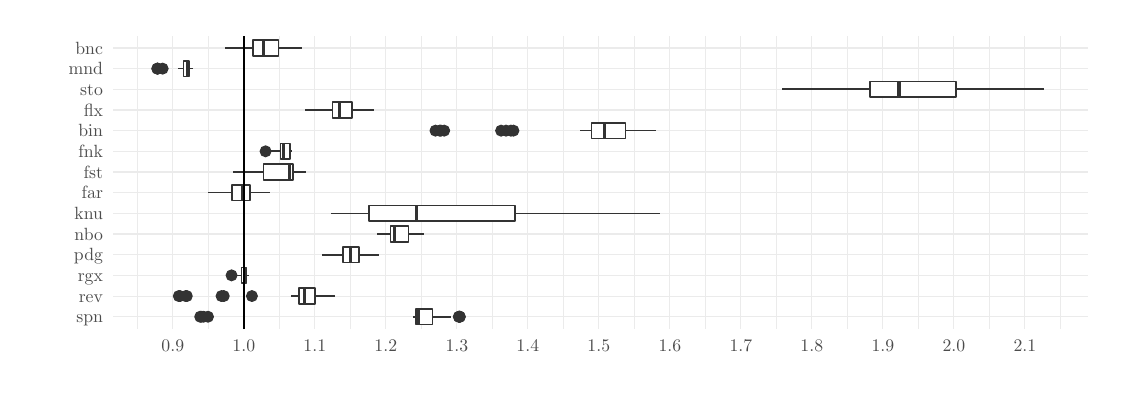
\begin{tikzpicture}[x=1pt,y=1pt]
\definecolor{fillColor}{RGB}{255,255,255}
\path[use as bounding box,fill=fillColor,fill opacity=0.00] (0,0) rectangle (390.26,130.09);
\begin{scope}
\path[clip] ( 30.80, 21.16) rectangle (383.14,127.24);
\definecolor{drawColor}{gray}{0.92}

\path[draw=drawColor,line width= 0.2pt,line join=round] ( 39.61, 21.16) --
	( 39.61,127.24);

\path[draw=drawColor,line width= 0.2pt,line join=round] ( 65.27, 21.16) --
	( 65.27,127.24);

\path[draw=drawColor,line width= 0.2pt,line join=round] ( 90.93, 21.16) --
	( 90.93,127.24);

\path[draw=drawColor,line width= 0.2pt,line join=round] (116.58, 21.16) --
	(116.58,127.24);

\path[draw=drawColor,line width= 0.2pt,line join=round] (142.24, 21.16) --
	(142.24,127.24);

\path[draw=drawColor,line width= 0.2pt,line join=round] (167.90, 21.16) --
	(167.90,127.24);

\path[draw=drawColor,line width= 0.2pt,line join=round] (193.55, 21.16) --
	(193.55,127.24);

\path[draw=drawColor,line width= 0.2pt,line join=round] (219.21, 21.16) --
	(219.21,127.24);

\path[draw=drawColor,line width= 0.2pt,line join=round] (244.87, 21.16) --
	(244.87,127.24);

\path[draw=drawColor,line width= 0.2pt,line join=round] (270.52, 21.16) --
	(270.52,127.24);

\path[draw=drawColor,line width= 0.2pt,line join=round] (296.18, 21.16) --
	(296.18,127.24);

\path[draw=drawColor,line width= 0.2pt,line join=round] (321.84, 21.16) --
	(321.84,127.24);

\path[draw=drawColor,line width= 0.2pt,line join=round] (347.50, 21.16) --
	(347.50,127.24);

\path[draw=drawColor,line width= 0.2pt,line join=round] (373.15, 21.16) --
	(373.15,127.24);

\path[draw=drawColor,line width= 0.4pt,line join=round] ( 30.80, 25.64) --
	(383.14, 25.64);

\path[draw=drawColor,line width= 0.4pt,line join=round] ( 30.80, 33.11) --
	(383.14, 33.11);

\path[draw=drawColor,line width= 0.4pt,line join=round] ( 30.80, 40.59) --
	(383.14, 40.59);

\path[draw=drawColor,line width= 0.4pt,line join=round] ( 30.80, 48.06) --
	(383.14, 48.06);

\path[draw=drawColor,line width= 0.4pt,line join=round] ( 30.80, 55.53) --
	(383.14, 55.53);

\path[draw=drawColor,line width= 0.4pt,line join=round] ( 30.80, 63.00) --
	(383.14, 63.00);

\path[draw=drawColor,line width= 0.4pt,line join=round] ( 30.80, 70.47) --
	(383.14, 70.47);

\path[draw=drawColor,line width= 0.4pt,line join=round] ( 30.80, 77.94) --
	(383.14, 77.94);

\path[draw=drawColor,line width= 0.4pt,line join=round] ( 30.80, 85.41) --
	(383.14, 85.41);

\path[draw=drawColor,line width= 0.4pt,line join=round] ( 30.80, 92.88) --
	(383.14, 92.88);

\path[draw=drawColor,line width= 0.4pt,line join=round] ( 30.80,100.35) --
	(383.14,100.35);

\path[draw=drawColor,line width= 0.4pt,line join=round] ( 30.80,107.82) --
	(383.14,107.82);

\path[draw=drawColor,line width= 0.4pt,line join=round] ( 30.80,115.29) --
	(383.14,115.29);

\path[draw=drawColor,line width= 0.4pt,line join=round] ( 30.80,122.76) --
	(383.14,122.76);

\path[draw=drawColor,line width= 0.4pt,line join=round] ( 52.44, 21.16) --
	( 52.44,127.24);

\path[draw=drawColor,line width= 0.4pt,line join=round] ( 78.10, 21.16) --
	( 78.10,127.24);

\path[draw=drawColor,line width= 0.4pt,line join=round] (103.75, 21.16) --
	(103.75,127.24);

\path[draw=drawColor,line width= 0.4pt,line join=round] (129.41, 21.16) --
	(129.41,127.24);

\path[draw=drawColor,line width= 0.4pt,line join=round] (155.07, 21.16) --
	(155.07,127.24);

\path[draw=drawColor,line width= 0.4pt,line join=round] (180.72, 21.16) --
	(180.72,127.24);

\path[draw=drawColor,line width= 0.4pt,line join=round] (206.38, 21.16) --
	(206.38,127.24);

\path[draw=drawColor,line width= 0.4pt,line join=round] (232.04, 21.16) --
	(232.04,127.24);

\path[draw=drawColor,line width= 0.4pt,line join=round] (257.70, 21.16) --
	(257.70,127.24);

\path[draw=drawColor,line width= 0.4pt,line join=round] (283.35, 21.16) --
	(283.35,127.24);

\path[draw=drawColor,line width= 0.4pt,line join=round] (309.01, 21.16) --
	(309.01,127.24);

\path[draw=drawColor,line width= 0.4pt,line join=round] (334.67, 21.16) --
	(334.67,127.24);

\path[draw=drawColor,line width= 0.4pt,line join=round] (360.32, 21.16) --
	(360.32,127.24);
\definecolor{drawColor}{gray}{0.20}
\definecolor{fillColor}{gray}{0.20}

\path[draw=drawColor,line width= 0.4pt,line join=round,line cap=round,fill=fillColor] (156.15, 25.64) circle (  1.96);

\path[draw=drawColor,line width= 0.4pt,line join=round,line cap=round,fill=fillColor] (156.12, 25.64) circle (  1.96);

\path[draw=drawColor,line width= 0.4pt,line join=round,line cap=round,fill=fillColor] (155.99, 25.64) circle (  1.96);

\path[draw=drawColor,line width= 0.4pt,line join=round,line cap=round,fill=fillColor] (155.93, 25.64) circle (  1.96);

\path[draw=drawColor,line width= 0.4pt,line join=round,line cap=round,fill=fillColor] (155.78, 25.64) circle (  1.96);

\path[draw=drawColor,line width= 0.4pt,line join=round,line cap=round,fill=fillColor] ( 65.16, 25.64) circle (  1.96);

\path[draw=drawColor,line width= 0.4pt,line join=round,line cap=round,fill=fillColor] ( 63.52, 25.64) circle (  1.96);

\path[draw=drawColor,line width= 0.4pt,line join=round,line cap=round,fill=fillColor] ( 62.73, 25.64) circle (  1.96);

\path[draw=drawColor,line width= 0.4pt,line join=round,line cap=round,fill=fillColor] ( 62.34, 25.64) circle (  1.96);

\path[draw=drawColor,line width= 0.6pt,line join=round] (146.25, 25.64) -- (152.79, 25.64);

\path[draw=drawColor,line width= 0.6pt,line join=round] (140.37, 25.64) -- (139.26, 25.64);
\definecolor{fillColor}{RGB}{255,255,255}

\path[draw=drawColor,line width= 0.6pt,line join=round,line cap=round,fill=fillColor] (146.25, 22.84) --
	(140.37, 22.84) --
	(140.37, 28.45) --
	(146.25, 28.45) --
	(146.25, 22.84) --
	cycle;

\path[draw=drawColor,line width= 1.1pt,line join=round] (141.25, 22.84) -- (141.25, 28.45);
\definecolor{fillColor}{gray}{0.20}

\path[draw=drawColor,line width= 0.4pt,line join=round,line cap=round,fill=fillColor] ( 81.03, 33.11) circle (  1.96);

\path[draw=drawColor,line width= 0.4pt,line join=round,line cap=round,fill=fillColor] ( 70.85, 33.11) circle (  1.96);

\path[draw=drawColor,line width= 0.4pt,line join=round,line cap=round,fill=fillColor] ( 70.05, 33.11) circle (  1.96);

\path[draw=drawColor,line width= 0.4pt,line join=round,line cap=round,fill=fillColor] ( 57.50, 33.11) circle (  1.96);

\path[draw=drawColor,line width= 0.4pt,line join=round,line cap=round,fill=fillColor] ( 57.11, 33.11) circle (  1.96);

\path[draw=drawColor,line width= 0.4pt,line join=round,line cap=round,fill=fillColor] ( 55.03, 33.11) circle (  1.96);

\path[draw=drawColor,line width= 0.4pt,line join=round,line cap=round,fill=fillColor] ( 54.61, 33.11) circle (  1.96);

\path[draw=drawColor,line width= 0.6pt,line join=round] (103.83, 33.11) -- (110.91, 33.11);

\path[draw=drawColor,line width= 0.6pt,line join=round] ( 98.16, 33.11) -- ( 95.23, 33.11);
\definecolor{fillColor}{RGB}{255,255,255}

\path[draw=drawColor,line width= 0.6pt,line join=round,line cap=round,fill=fillColor] (103.83, 30.31) --
	( 98.16, 30.31) --
	( 98.16, 35.92) --
	(103.83, 35.92) --
	(103.83, 30.31) --
	cycle;

\path[draw=drawColor,line width= 1.1pt,line join=round] (100.11, 30.31) -- (100.11, 35.92);
\definecolor{fillColor}{gray}{0.20}

\path[draw=drawColor,line width= 0.4pt,line join=round,line cap=round,fill=fillColor] ( 73.67, 40.59) circle (  1.96);

\path[draw=drawColor,line width= 0.6pt,line join=round] ( 79.10, 40.59) -- ( 79.80, 40.59);

\path[draw=drawColor,line width= 0.6pt,line join=round] ( 77.25, 40.59) -- ( 74.95, 40.59);
\definecolor{fillColor}{RGB}{255,255,255}

\path[draw=drawColor,line width= 0.6pt,line join=round,line cap=round,fill=fillColor] ( 79.10, 37.78) --
	( 77.25, 37.78) --
	( 77.25, 43.39) --
	( 79.10, 43.39) --
	( 79.10, 37.78) --
	cycle;

\path[draw=drawColor,line width= 1.1pt,line join=round] ( 78.68, 37.78) -- ( 78.68, 43.39);

\path[draw=drawColor,line width= 0.6pt,line join=round] (119.62, 48.06) -- (126.98, 48.06);

\path[draw=drawColor,line width= 0.6pt,line join=round] (113.92, 48.06) -- (106.44, 48.06);

\path[draw=drawColor,line width= 0.6pt,line join=round,line cap=round,fill=fillColor] (119.62, 45.25) --
	(113.92, 45.25) --
	(113.92, 50.86) --
	(119.62, 50.86) --
	(119.62, 45.25) --
	cycle;

\path[draw=drawColor,line width= 1.1pt,line join=round] (116.71, 45.25) -- (116.71, 50.86);

\path[draw=drawColor,line width= 0.6pt,line join=round] (137.64, 55.53) -- (143.32, 55.53);

\path[draw=drawColor,line width= 0.6pt,line join=round] (131.11, 55.53) -- (126.10, 55.53);

\path[draw=drawColor,line width= 0.6pt,line join=round,line cap=round,fill=fillColor] (137.64, 52.72) --
	(131.11, 52.72) --
	(131.11, 58.33) --
	(137.64, 58.33) --
	(137.64, 52.72) --
	cycle;

\path[draw=drawColor,line width= 1.1pt,line join=round] (132.52, 52.72) -- (132.52, 58.33);

\path[draw=drawColor,line width= 0.6pt,line join=round] (176.13, 63.00) -- (228.50, 63.00);

\path[draw=drawColor,line width= 0.6pt,line join=round] (123.24, 63.00) -- (109.43, 63.00);

\path[draw=drawColor,line width= 0.6pt,line join=round,line cap=round,fill=fillColor] (176.13, 60.19) --
	(123.24, 60.19) --
	(123.24, 65.80) --
	(176.13, 65.80) --
	(176.13, 60.19) --
	cycle;

\path[draw=drawColor,line width= 1.1pt,line join=round] (140.40, 60.19) -- (140.40, 65.80);

\path[draw=drawColor,line width= 0.6pt,line join=round] ( 80.43, 70.47) -- ( 87.42, 70.47);

\path[draw=drawColor,line width= 0.6pt,line join=round] ( 73.78, 70.47) -- ( 65.12, 70.47);

\path[draw=drawColor,line width= 0.6pt,line join=round,line cap=round,fill=fillColor] ( 80.43, 67.66) --
	( 73.78, 67.66) --
	( 73.78, 73.27) --
	( 80.43, 73.27) --
	( 80.43, 67.66) --
	cycle;

\path[draw=drawColor,line width= 1.1pt,line join=round] ( 77.51, 67.66) -- ( 77.51, 73.27);

\path[draw=drawColor,line width= 0.6pt,line join=round] ( 95.85, 77.94) -- (100.61, 77.94);

\path[draw=drawColor,line width= 0.6pt,line join=round] ( 85.22, 77.94) -- ( 74.17, 77.94);

\path[draw=drawColor,line width= 0.6pt,line join=round,line cap=round,fill=fillColor] ( 95.85, 75.14) --
	( 85.22, 75.14) --
	( 85.22, 80.74) --
	( 95.85, 80.74) --
	( 95.85, 75.14) --
	cycle;

\path[draw=drawColor,line width= 1.1pt,line join=round] ( 94.47, 75.14) -- ( 94.47, 80.74);
\definecolor{fillColor}{gray}{0.20}

\path[draw=drawColor,line width= 0.4pt,line join=round,line cap=round,fill=fillColor] ( 85.96, 85.41) circle (  1.96);

\path[draw=drawColor,line width= 0.6pt,line join=round] ( 94.71, 85.41) -- ( 95.48, 85.41);

\path[draw=drawColor,line width= 0.6pt,line join=round] ( 91.33, 85.41) -- ( 87.02, 85.41);
\definecolor{fillColor}{RGB}{255,255,255}

\path[draw=drawColor,line width= 0.6pt,line join=round,line cap=round,fill=fillColor] ( 94.71, 82.61) --
	( 91.33, 82.61) --
	( 91.33, 88.21) --
	( 94.71, 88.21) --
	( 94.71, 82.61) --
	cycle;

\path[draw=drawColor,line width= 1.1pt,line join=round] ( 92.53, 82.61) -- ( 92.53, 88.21);
\definecolor{fillColor}{gray}{0.20}

\path[draw=drawColor,line width= 0.4pt,line join=round,line cap=round,fill=fillColor] (175.53, 92.88) circle (  1.96);

\path[draw=drawColor,line width= 0.4pt,line join=round,line cap=round,fill=fillColor] (174.60, 92.88) circle (  1.96);

\path[draw=drawColor,line width= 0.4pt,line join=round,line cap=round,fill=fillColor] (172.86, 92.88) circle (  1.96);

\path[draw=drawColor,line width= 0.4pt,line join=round,line cap=round,fill=fillColor] (171.07, 92.88) circle (  1.96);

\path[draw=drawColor,line width= 0.4pt,line join=round,line cap=round,fill=fillColor] (150.51, 92.88) circle (  1.96);

\path[draw=drawColor,line width= 0.4pt,line join=round,line cap=round,fill=fillColor] (149.30, 92.88) circle (  1.96);

\path[draw=drawColor,line width= 0.4pt,line join=round,line cap=round,fill=fillColor] (148.89, 92.88) circle (  1.96);

\path[draw=drawColor,line width= 0.4pt,line join=round,line cap=round,fill=fillColor] (147.36, 92.88) circle (  1.96);

\path[draw=drawColor,line width= 0.6pt,line join=round] (215.97, 92.88) -- (227.06, 92.88);

\path[draw=drawColor,line width= 0.6pt,line join=round] (203.77, 92.88) -- (199.42, 92.88);
\definecolor{fillColor}{RGB}{255,255,255}

\path[draw=drawColor,line width= 0.6pt,line join=round,line cap=round,fill=fillColor] (215.97, 90.08) --
	(203.77, 90.08) --
	(203.77, 95.68) --
	(215.97, 95.68) --
	(215.97, 90.08) --
	cycle;

\path[draw=drawColor,line width= 1.1pt,line join=round] (208.57, 90.08) -- (208.57, 95.68);

\path[draw=drawColor,line width= 0.6pt,line join=round] (117.23,100.35) -- (125.27,100.35);

\path[draw=drawColor,line width= 0.6pt,line join=round] (110.12,100.35) -- (100.09,100.35);

\path[draw=drawColor,line width= 0.6pt,line join=round,line cap=round,fill=fillColor] (117.23, 97.55) --
	(110.12, 97.55) --
	(110.12,103.15) --
	(117.23,103.15) --
	(117.23, 97.55) --
	cycle;

\path[draw=drawColor,line width= 1.1pt,line join=round] (112.68, 97.55) -- (112.68,103.15);

\path[draw=drawColor,line width= 0.6pt,line join=round] (335.48,107.82) -- (367.13,107.82);

\path[draw=drawColor,line width= 0.6pt,line join=round] (304.34,107.82) -- (272.46,107.82);

\path[draw=drawColor,line width= 0.6pt,line join=round,line cap=round,fill=fillColor] (335.48,105.02) --
	(304.34,105.02) --
	(304.34,110.62) --
	(335.48,110.62) --
	(335.48,105.02) --
	cycle;

\path[draw=drawColor,line width= 1.1pt,line join=round] (314.85,105.02) -- (314.85,110.62);
\definecolor{fillColor}{gray}{0.20}

\path[draw=drawColor,line width= 0.4pt,line join=round,line cap=round,fill=fillColor] ( 48.77,115.29) circle (  1.96);

\path[draw=drawColor,line width= 0.4pt,line join=round,line cap=round,fill=fillColor] ( 47.00,115.29) circle (  1.96);

\path[draw=drawColor,line width= 0.4pt,line join=round,line cap=round,fill=fillColor] ( 46.92,115.29) circle (  1.96);

\path[draw=drawColor,line width= 0.4pt,line join=round,line cap=round,fill=fillColor] ( 46.81,115.29) circle (  1.96);

\path[draw=drawColor,line width= 0.6pt,line join=round] ( 58.27,115.29) -- ( 59.68,115.29);

\path[draw=drawColor,line width= 0.6pt,line join=round] ( 56.36,115.29) -- ( 54.49,115.29);
\definecolor{fillColor}{RGB}{255,255,255}

\path[draw=drawColor,line width= 0.6pt,line join=round,line cap=round,fill=fillColor] ( 58.27,112.49) --
	( 56.36,112.49) --
	( 56.36,118.09) --
	( 58.27,118.09) --
	( 58.27,112.49) --
	cycle;

\path[draw=drawColor,line width= 1.1pt,line join=round] ( 57.71,112.49) -- ( 57.71,118.09);

\path[draw=drawColor,line width= 0.6pt,line join=round] ( 90.59,122.76) -- ( 99.03,122.76);

\path[draw=drawColor,line width= 0.6pt,line join=round] ( 81.46,122.76) -- ( 71.38,122.76);

\path[draw=drawColor,line width= 0.6pt,line join=round,line cap=round,fill=fillColor] ( 90.59,119.96) --
	( 81.46,119.96) --
	( 81.46,125.56) --
	( 90.59,125.56) --
	( 90.59,119.96) --
	cycle;

\path[draw=drawColor,line width= 1.1pt,line join=round] ( 85.21,119.96) -- ( 85.21,125.56);
\definecolor{drawColor}{RGB}{0,0,0}

\path[draw=drawColor,line width= 0.6pt,line join=round] ( 78.10, 21.16) -- ( 78.10,127.24);
\end{scope}
\begin{scope}
\path[clip] (  0.00,  0.00) rectangle (390.26,130.09);
\definecolor{drawColor}{gray}{0.30}

\node[text=drawColor,anchor=base east,inner sep=0pt, outer sep=0pt, scale=  0.64] at ( 27.20, 23.44) {spn};

\node[text=drawColor,anchor=base east,inner sep=0pt, outer sep=0pt, scale=  0.64] at ( 27.20, 30.91) {rev};

\node[text=drawColor,anchor=base east,inner sep=0pt, outer sep=0pt, scale=  0.64] at ( 27.20, 38.38) {rgx};

\node[text=drawColor,anchor=base east,inner sep=0pt, outer sep=0pt, scale=  0.64] at ( 27.20, 45.85) {pdg};

\node[text=drawColor,anchor=base east,inner sep=0pt, outer sep=0pt, scale=  0.64] at ( 27.20, 53.32) {nbo};

\node[text=drawColor,anchor=base east,inner sep=0pt, outer sep=0pt, scale=  0.64] at ( 27.20, 60.79) {knu};

\node[text=drawColor,anchor=base east,inner sep=0pt, outer sep=0pt, scale=  0.64] at ( 27.20, 68.26) {far};

\node[text=drawColor,anchor=base east,inner sep=0pt, outer sep=0pt, scale=  0.64] at ( 27.20, 75.73) {fst};

\node[text=drawColor,anchor=base east,inner sep=0pt, outer sep=0pt, scale=  0.64] at ( 27.20, 83.20) {fnk};

\node[text=drawColor,anchor=base east,inner sep=0pt, outer sep=0pt, scale=  0.64] at ( 27.20, 90.67) {bin};

\node[text=drawColor,anchor=base east,inner sep=0pt, outer sep=0pt, scale=  0.64] at ( 27.20, 98.14) {flx};

\node[text=drawColor,anchor=base east,inner sep=0pt, outer sep=0pt, scale=  0.64] at ( 27.20,105.61) {sto};

\node[text=drawColor,anchor=base east,inner sep=0pt, outer sep=0pt, scale=  0.64] at ( 27.20,113.08) {mnd};

\node[text=drawColor,anchor=base east,inner sep=0pt, outer sep=0pt, scale=  0.64] at ( 27.20,120.55) {bnc};
\end{scope}
\begin{scope}
\path[clip] (  0.00,  0.00) rectangle (390.26,130.09);
\definecolor{drawColor}{gray}{0.30}

\node[text=drawColor,anchor=base,inner sep=0pt, outer sep=0pt, scale=  0.64] at ( 52.44, 13.15) {0.9};

\node[text=drawColor,anchor=base,inner sep=0pt, outer sep=0pt, scale=  0.64] at ( 78.10, 13.15) {1.0};

\node[text=drawColor,anchor=base,inner sep=0pt, outer sep=0pt, scale=  0.64] at (103.75, 13.15) {1.1};

\node[text=drawColor,anchor=base,inner sep=0pt, outer sep=0pt, scale=  0.64] at (129.41, 13.15) {1.2};

\node[text=drawColor,anchor=base,inner sep=0pt, outer sep=0pt, scale=  0.64] at (155.07, 13.15) {1.3};

\node[text=drawColor,anchor=base,inner sep=0pt, outer sep=0pt, scale=  0.64] at (180.72, 13.15) {1.4};

\node[text=drawColor,anchor=base,inner sep=0pt, outer sep=0pt, scale=  0.64] at (206.38, 13.15) {1.5};

\node[text=drawColor,anchor=base,inner sep=0pt, outer sep=0pt, scale=  0.64] at (232.04, 13.15) {1.6};

\node[text=drawColor,anchor=base,inner sep=0pt, outer sep=0pt, scale=  0.64] at (257.70, 13.15) {1.7};

\node[text=drawColor,anchor=base,inner sep=0pt, outer sep=0pt, scale=  0.64] at (283.35, 13.15) {1.8};

\node[text=drawColor,anchor=base,inner sep=0pt, outer sep=0pt, scale=  0.64] at (309.01, 13.15) {1.9};

\node[text=drawColor,anchor=base,inner sep=0pt, outer sep=0pt, scale=  0.64] at (334.67, 13.15) {2.0};

\node[text=drawColor,anchor=base,inner sep=0pt, outer sep=0pt, scale=  0.64] at (360.32, 13.15) {2.1};
\end{scope}
\end{tikzpicture}

  \caption{Speedup of \Rshstrict}
  \label{fig:speedup}
\end{figure}

First, we compare \Rsh against \Rshstrict. This experiment estimates the end-to-end
improvement on performance that a change to eager semantics in the R language
would have on \Rsh. The execution times were measured with $t_e = 4, t_i = 25$.
\autoref{fig:speedup} shows a boxplot for the execution times of \Rsh-strict,
normalized to \Rsh. Overall, we observe a mean speedup of
\speedupRshStrict, ranging from \speedupRshStrictMin to \speedupRshStrictMax.
For \speedupRshStrictSignificant out of \benchmarkSuiteSize benchmarks we measure a significant increase in performance.
%
\begin{figure}[h]
  \centering
  % Created by tikzDevice version 0.12.3.1 on 2021-04-14 13:17:10
% !TEX encoding = UTF-8 Unicode
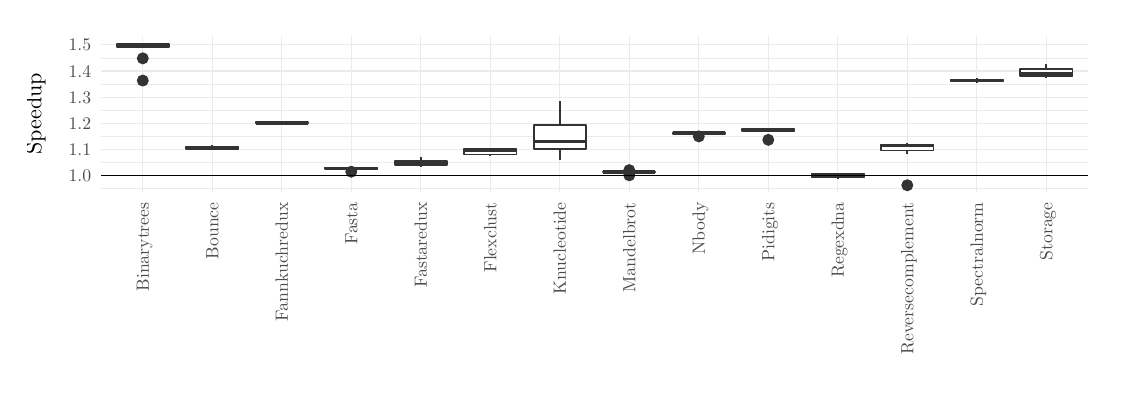
\begin{tikzpicture}[x=1pt,y=1pt]
\definecolor{fillColor}{RGB}{255,255,255}
\path[use as bounding box,fill=fillColor,fill opacity=0.00] (0,0) rectangle (390.26,130.09);
\begin{scope}
\path[clip] ( 26.53, 70.57) rectangle (383.14,127.24);
\definecolor{drawColor}{gray}{0.92}

\path[draw=drawColor,line width= 0.2pt,line join=round] ( 26.53, 71.98) --
	(383.14, 71.98);

\path[draw=drawColor,line width= 0.2pt,line join=round] ( 26.53, 81.42) --
	(383.14, 81.42);

\path[draw=drawColor,line width= 0.2pt,line join=round] ( 26.53, 90.85) --
	(383.14, 90.85);

\path[draw=drawColor,line width= 0.2pt,line join=round] ( 26.53,100.29) --
	(383.14,100.29);

\path[draw=drawColor,line width= 0.2pt,line join=round] ( 26.53,109.72) --
	(383.14,109.72);

\path[draw=drawColor,line width= 0.2pt,line join=round] ( 26.53,119.16) --
	(383.14,119.16);

\path[draw=drawColor,line width= 0.4pt,line join=round] ( 26.53, 76.70) --
	(383.14, 76.70);

\path[draw=drawColor,line width= 0.4pt,line join=round] ( 26.53, 86.14) --
	(383.14, 86.14);

\path[draw=drawColor,line width= 0.4pt,line join=round] ( 26.53, 95.57) --
	(383.14, 95.57);

\path[draw=drawColor,line width= 0.4pt,line join=round] ( 26.53,105.00) --
	(383.14,105.00);

\path[draw=drawColor,line width= 0.4pt,line join=round] ( 26.53,114.44) --
	(383.14,114.44);

\path[draw=drawColor,line width= 0.4pt,line join=round] ( 26.53,123.87) --
	(383.14,123.87);

\path[draw=drawColor,line width= 0.4pt,line join=round] ( 41.60, 70.57) --
	( 41.60,127.24);

\path[draw=drawColor,line width= 0.4pt,line join=round] ( 66.71, 70.57) --
	( 66.71,127.24);

\path[draw=drawColor,line width= 0.4pt,line join=round] ( 91.83, 70.57) --
	( 91.83,127.24);

\path[draw=drawColor,line width= 0.4pt,line join=round] (116.94, 70.57) --
	(116.94,127.24);

\path[draw=drawColor,line width= 0.4pt,line join=round] (142.05, 70.57) --
	(142.05,127.24);

\path[draw=drawColor,line width= 0.4pt,line join=round] (167.17, 70.57) --
	(167.17,127.24);

\path[draw=drawColor,line width= 0.4pt,line join=round] (192.28, 70.57) --
	(192.28,127.24);

\path[draw=drawColor,line width= 0.4pt,line join=round] (217.39, 70.57) --
	(217.39,127.24);

\path[draw=drawColor,line width= 0.4pt,line join=round] (242.51, 70.57) --
	(242.51,127.24);

\path[draw=drawColor,line width= 0.4pt,line join=round] (267.62, 70.57) --
	(267.62,127.24);

\path[draw=drawColor,line width= 0.4pt,line join=round] (292.74, 70.57) --
	(292.74,127.24);

\path[draw=drawColor,line width= 0.4pt,line join=round] (317.85, 70.57) --
	(317.85,127.24);

\path[draw=drawColor,line width= 0.4pt,line join=round] (342.96, 70.57) --
	(342.96,127.24);

\path[draw=drawColor,line width= 0.4pt,line join=round] (368.08, 70.57) --
	(368.08,127.24);
\definecolor{drawColor}{gray}{0.20}
\definecolor{fillColor}{gray}{0.20}

\path[draw=drawColor,line width= 0.4pt,line join=round,line cap=round,fill=fillColor] ( 41.60,119.00) circle (  1.96);

\path[draw=drawColor,line width= 0.4pt,line join=round,line cap=round,fill=fillColor] ( 41.60,110.98) circle (  1.96);

\path[draw=drawColor,line width= 0.6pt,line join=round] ( 41.60,124.07) -- ( 41.60,124.66);

\path[draw=drawColor,line width= 0.6pt,line join=round] ( 41.60,123.05) -- ( 41.60,123.02);
\definecolor{fillColor}{RGB}{255,255,255}

\path[draw=drawColor,line width= 0.6pt,line join=round,line cap=round,fill=fillColor] ( 32.18,124.07) --
	( 32.18,123.05) --
	( 51.02,123.05) --
	( 51.02,124.07) --
	( 32.18,124.07) --
	cycle;

\path[draw=drawColor,line width= 1.1pt,line join=round] ( 32.18,123.28) -- ( 51.02,123.28);

\path[draw=drawColor,line width= 0.6pt,line join=round] ( 66.71, 87.10) -- ( 66.71, 87.62);

\path[draw=drawColor,line width= 0.6pt,line join=round] ( 66.71, 86.23) -- ( 66.71, 85.92);

\path[draw=drawColor,line width= 0.6pt,line join=round,line cap=round,fill=fillColor] ( 57.30, 87.10) --
	( 57.30, 86.23) --
	( 76.13, 86.23) --
	( 76.13, 87.10) --
	( 57.30, 87.10) --
	cycle;

\path[draw=drawColor,line width= 1.1pt,line join=round] ( 57.30, 86.67) -- ( 76.13, 86.67);

\path[draw=drawColor,line width= 0.6pt,line join=round] ( 91.83, 96.08) -- ( 91.83, 96.51);

\path[draw=drawColor,line width= 0.6pt,line join=round] ( 91.83, 95.52) -- ( 91.83, 95.13);

\path[draw=drawColor,line width= 0.6pt,line join=round,line cap=round,fill=fillColor] ( 82.41, 96.08) --
	( 82.41, 95.52) --
	(101.24, 95.52) --
	(101.24, 96.08) --
	( 82.41, 96.08) --
	cycle;

\path[draw=drawColor,line width= 1.1pt,line join=round] ( 82.41, 95.65) -- (101.24, 95.65);
\definecolor{fillColor}{gray}{0.20}

\path[draw=drawColor,line width= 0.4pt,line join=round,line cap=round,fill=fillColor] (116.94, 78.04) circle (  1.96);

\path[draw=drawColor,line width= 0.6pt,line join=round] (116.94, 79.62) -- (116.94, 80.13);

\path[draw=drawColor,line width= 0.6pt,line join=round] (116.94, 79.07) -- (116.94, 78.60);
\definecolor{fillColor}{RGB}{255,255,255}

\path[draw=drawColor,line width= 0.6pt,line join=round,line cap=round,fill=fillColor] (107.52, 79.62) --
	(107.52, 79.07) --
	(126.36, 79.07) --
	(126.36, 79.62) --
	(107.52, 79.62) --
	cycle;

\path[draw=drawColor,line width= 1.1pt,line join=round] (107.52, 79.28) -- (126.36, 79.28);

\path[draw=drawColor,line width= 0.6pt,line join=round] (142.05, 81.94) -- (142.05, 83.46);

\path[draw=drawColor,line width= 0.6pt,line join=round] (142.05, 80.49) -- (142.05, 79.85);

\path[draw=drawColor,line width= 0.6pt,line join=round,line cap=round,fill=fillColor] (132.64, 81.94) --
	(132.64, 80.49) --
	(151.47, 80.49) --
	(151.47, 81.94) --
	(132.64, 81.94) --
	cycle;

\path[draw=drawColor,line width= 1.1pt,line join=round] (132.64, 81.42) -- (151.47, 81.42);

\path[draw=drawColor,line width= 0.6pt,line join=round] (167.17, 86.16) -- (167.17, 86.56);

\path[draw=drawColor,line width= 0.6pt,line join=round] (167.17, 84.31) -- (167.17, 83.69);

\path[draw=drawColor,line width= 0.6pt,line join=round,line cap=round,fill=fillColor] (157.75, 86.16) --
	(157.75, 84.31) --
	(176.59, 84.31) --
	(176.59, 86.16) --
	(157.75, 86.16) --
	cycle;

\path[draw=drawColor,line width= 1.1pt,line join=round] (157.75, 85.66) -- (176.59, 85.66);

\path[draw=drawColor,line width= 0.6pt,line join=round] (192.28, 94.98) -- (192.28,103.56);

\path[draw=drawColor,line width= 0.6pt,line join=round] (192.28, 86.21) -- (192.28, 82.24);

\path[draw=drawColor,line width= 0.6pt,line join=round,line cap=round,fill=fillColor] (182.86, 94.98) --
	(182.86, 86.21) --
	(201.70, 86.21) --
	(201.70, 94.98) --
	(182.86, 94.98) --
	cycle;

\path[draw=drawColor,line width= 1.1pt,line join=round] (182.86, 89.08) -- (201.70, 89.08);
\definecolor{fillColor}{gray}{0.20}

\path[draw=drawColor,line width= 0.4pt,line join=round,line cap=round,fill=fillColor] (217.39, 78.61) circle (  1.96);

\path[draw=drawColor,line width= 0.4pt,line join=round,line cap=round,fill=fillColor] (217.39, 76.74) circle (  1.96);

\path[draw=drawColor,line width= 0.6pt,line join=round] (217.39, 78.09) -- (217.39, 78.13);

\path[draw=drawColor,line width= 0.6pt,line join=round] (217.39, 77.86) -- (217.39, 77.59);
\definecolor{fillColor}{RGB}{255,255,255}

\path[draw=drawColor,line width= 0.6pt,line join=round,line cap=round,fill=fillColor] (207.98, 78.09) --
	(207.98, 77.86) --
	(226.81, 77.86) --
	(226.81, 78.09) --
	(207.98, 78.09) --
	cycle;

\path[draw=drawColor,line width= 1.1pt,line join=round] (207.98, 77.94) -- (226.81, 77.94);
\definecolor{fillColor}{gray}{0.20}

\path[draw=drawColor,line width= 0.4pt,line join=round,line cap=round,fill=fillColor] (242.51, 90.80) circle (  1.96);

\path[draw=drawColor,line width= 0.6pt,line join=round] (242.51, 92.21) -- (242.51, 92.32);

\path[draw=drawColor,line width= 0.6pt,line join=round] (242.51, 91.78) -- (242.51, 91.16);
\definecolor{fillColor}{RGB}{255,255,255}

\path[draw=drawColor,line width= 0.6pt,line join=round,line cap=round,fill=fillColor] (233.09, 92.21) --
	(233.09, 91.78) --
	(251.93, 91.78) --
	(251.93, 92.21) --
	(233.09, 92.21) --
	cycle;

\path[draw=drawColor,line width= 1.1pt,line join=round] (233.09, 92.07) -- (251.93, 92.07);
\definecolor{fillColor}{gray}{0.20}

\path[draw=drawColor,line width= 0.4pt,line join=round,line cap=round,fill=fillColor] (267.62, 89.56) circle (  1.96);

\path[draw=drawColor,line width= 0.6pt,line join=round] (267.62, 93.46) -- (267.62, 93.69);

\path[draw=drawColor,line width= 0.6pt,line join=round] (267.62, 92.73) -- (267.62, 92.57);
\definecolor{fillColor}{RGB}{255,255,255}

\path[draw=drawColor,line width= 0.6pt,line join=round,line cap=round,fill=fillColor] (258.20, 93.46) --
	(258.20, 92.73) --
	(277.04, 92.73) --
	(277.04, 93.46) --
	(258.20, 93.46) --
	cycle;

\path[draw=drawColor,line width= 1.1pt,line join=round] (258.20, 93.29) -- (277.04, 93.29);

\path[draw=drawColor,line width= 0.6pt,line join=round] (292.74, 77.36) -- (292.74, 77.50);

\path[draw=drawColor,line width= 0.6pt,line join=round] (292.74, 75.93) -- (292.74, 75.31);

\path[draw=drawColor,line width= 0.6pt,line join=round,line cap=round,fill=fillColor] (283.32, 77.36) --
	(283.32, 75.93) --
	(302.15, 75.93) --
	(302.15, 77.36) --
	(283.32, 77.36) --
	cycle;

\path[draw=drawColor,line width= 1.1pt,line join=round] (283.32, 76.68) -- (302.15, 76.68);
\definecolor{fillColor}{gray}{0.20}

\path[draw=drawColor,line width= 0.4pt,line join=round,line cap=round,fill=fillColor] (317.85, 73.15) circle (  1.96);

\path[draw=drawColor,line width= 0.6pt,line join=round] (317.85, 87.82) -- (317.85, 88.27);

\path[draw=drawColor,line width= 0.6pt,line join=round] (317.85, 85.75) -- (317.85, 84.30);
\definecolor{fillColor}{RGB}{255,255,255}

\path[draw=drawColor,line width= 0.6pt,line join=round,line cap=round,fill=fillColor] (308.43, 87.82) --
	(308.43, 85.75) --
	(327.27, 85.75) --
	(327.27, 87.82) --
	(308.43, 87.82) --
	cycle;

\path[draw=drawColor,line width= 1.1pt,line join=round] (308.43, 87.41) -- (327.27, 87.41);

\path[draw=drawColor,line width= 0.6pt,line join=round] (342.96,111.40) -- (342.96,111.74);

\path[draw=drawColor,line width= 0.6pt,line join=round] (342.96,110.58) -- (342.96,109.92);

\path[draw=drawColor,line width= 0.6pt,line join=round,line cap=round,fill=fillColor] (333.55,111.40) --
	(333.55,110.58) --
	(352.38,110.58) --
	(352.38,111.40) --
	(333.55,111.40) --
	cycle;

\path[draw=drawColor,line width= 1.1pt,line join=round] (333.55,111.17) -- (352.38,111.17);

\path[draw=drawColor,line width= 0.6pt,line join=round] (368.08,115.10) -- (368.08,116.89);

\path[draw=drawColor,line width= 0.6pt,line join=round] (368.08,112.52) -- (368.08,111.75);

\path[draw=drawColor,line width= 0.6pt,line join=round,line cap=round,fill=fillColor] (358.66,115.10) --
	(358.66,112.52) --
	(377.49,112.52) --
	(377.49,115.10) --
	(358.66,115.10) --
	cycle;

\path[draw=drawColor,line width= 1.1pt,line join=round] (358.66,113.65) -- (377.49,113.65);
\definecolor{drawColor}{RGB}{0,0,0}

\path[draw=drawColor,line width= 0.6pt,line join=round] ( 26.53, 76.70) -- (383.14, 76.70);
\end{scope}
\begin{scope}
\path[clip] (  0.00,  0.00) rectangle (390.26,130.09);
\definecolor{drawColor}{gray}{0.30}

\node[text=drawColor,anchor=base east,inner sep=0pt, outer sep=0pt, scale=  0.64] at ( 22.93, 74.50) {1.0};

\node[text=drawColor,anchor=base east,inner sep=0pt, outer sep=0pt, scale=  0.64] at ( 22.93, 83.93) {1.1};

\node[text=drawColor,anchor=base east,inner sep=0pt, outer sep=0pt, scale=  0.64] at ( 22.93, 93.37) {1.2};

\node[text=drawColor,anchor=base east,inner sep=0pt, outer sep=0pt, scale=  0.64] at ( 22.93,102.80) {1.3};

\node[text=drawColor,anchor=base east,inner sep=0pt, outer sep=0pt, scale=  0.64] at ( 22.93,112.24) {1.4};

\node[text=drawColor,anchor=base east,inner sep=0pt, outer sep=0pt, scale=  0.64] at ( 22.93,121.67) {1.5};
\end{scope}
\begin{scope}
\path[clip] (  0.00,  0.00) rectangle (390.26,130.09);
\definecolor{drawColor}{gray}{0.30}

\node[text=drawColor,rotate= 90.00,anchor=base east,inner sep=0pt, outer sep=0pt, scale=  0.64] at ( 43.80, 66.97) {Binarytrees};

\node[text=drawColor,rotate= 90.00,anchor=base east,inner sep=0pt, outer sep=0pt, scale=  0.64] at ( 68.92, 66.97) {Bounce};

\node[text=drawColor,rotate= 90.00,anchor=base east,inner sep=0pt, outer sep=0pt, scale=  0.64] at ( 94.03, 66.97) {Fannkuchredux};

\node[text=drawColor,rotate= 90.00,anchor=base east,inner sep=0pt, outer sep=0pt, scale=  0.64] at (119.14, 66.97) {Fasta};

\node[text=drawColor,rotate= 90.00,anchor=base east,inner sep=0pt, outer sep=0pt, scale=  0.64] at (144.26, 66.97) {Fastaredux};

\node[text=drawColor,rotate= 90.00,anchor=base east,inner sep=0pt, outer sep=0pt, scale=  0.64] at (169.37, 66.97) {Flexclust};

\node[text=drawColor,rotate= 90.00,anchor=base east,inner sep=0pt, outer sep=0pt, scale=  0.64] at (194.49, 66.97) {Knucleotide};

\node[text=drawColor,rotate= 90.00,anchor=base east,inner sep=0pt, outer sep=0pt, scale=  0.64] at (219.60, 66.97) {Mandelbrot};

\node[text=drawColor,rotate= 90.00,anchor=base east,inner sep=0pt, outer sep=0pt, scale=  0.64] at (244.71, 66.97) {Nbody};

\node[text=drawColor,rotate= 90.00,anchor=base east,inner sep=0pt, outer sep=0pt, scale=  0.64] at (269.83, 66.97) {Pidigits};

\node[text=drawColor,rotate= 90.00,anchor=base east,inner sep=0pt, outer sep=0pt, scale=  0.64] at (294.94, 66.97) {Regexdna};

\node[text=drawColor,rotate= 90.00,anchor=base east,inner sep=0pt, outer sep=0pt, scale=  0.64] at (320.05, 66.97) {Reversecomplement};

\node[text=drawColor,rotate= 90.00,anchor=base east,inner sep=0pt, outer sep=0pt, scale=  0.64] at (345.17, 66.97) {Spectralnorm};

\node[text=drawColor,rotate= 90.00,anchor=base east,inner sep=0pt, outer sep=0pt, scale=  0.64] at (370.28, 66.97) {Storage};
\end{scope}
\begin{scope}
\path[clip] (  0.00,  0.00) rectangle (390.26,130.09);
\definecolor{drawColor}{RGB}{0,0,0}

\node[text=drawColor,rotate= 90.00,anchor=base,inner sep=0pt, outer sep=0pt, scale=  0.80] at (  4.98, 98.91) {Speedup};
\end{scope}
\end{tikzpicture}

  \caption{Speedup of \Rshstrict without optimizations}
  \label{fig:speedup-bc}
\end{figure}
%
Then, we repeated the performance experiment, but with the second tier
optimizer completely disabled. Since this variant executes overall \rshBCSlowdown
slower, we chose to only run with $t_e = 1, t_i = 15$.
The results are presented in \autoref{fig:speedup-bc}. We found that the bytecode
interpreter also gains a speedup of \speedupBCRshStrict, ranging from
\speedupBCRshStrictMin to \speedupBCRshStrictMax.
%
Thus, we conclude that in our benchmark suite both a naive interpreter and a speculatively
optimizing native compiler, achieve better performance on a strict dialect of R.
Even though the speedup is very similar in numbers, the reasons seem to be
different at times. We will get back to that point in the discussion at the end of
this section.

\paragraph{Garbage Collection}

\begin{figure}[h]
  \centering
  % Created by tikzDevice version 0.12.3.1 on 2021-04-15 17:45:37
% !TEX encoding = UTF-8 Unicode
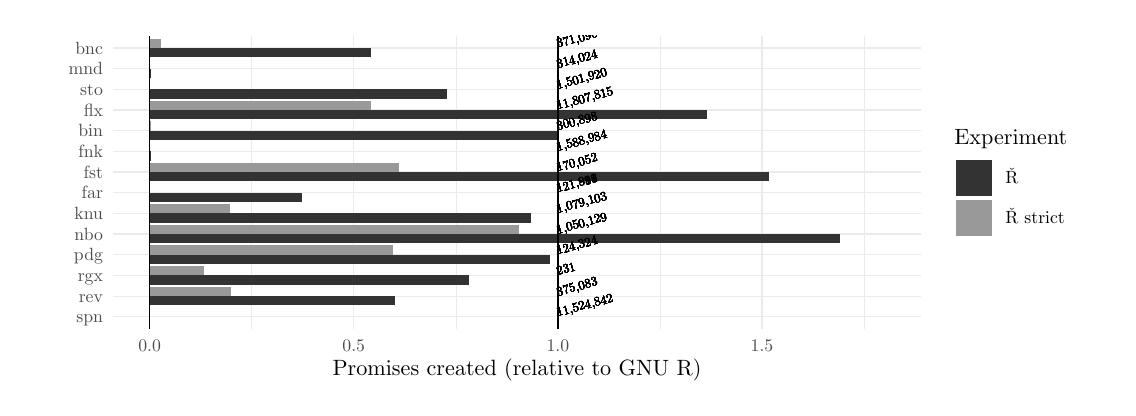
\begin{tikzpicture}[x=1pt,y=1pt]
\definecolor{fillColor}{RGB}{255,255,255}
\path[use as bounding box,fill=fillColor,fill opacity=0.00] (0,0) rectangle (390.26,130.09);
\begin{scope}
\path[clip] ( 30.80, 21.16) rectangle (322.87,127.24);
\definecolor{drawColor}{gray}{0.92}

\path[draw=drawColor,line width= 0.2pt,line join=round] ( 80.95, 21.16) --
	( 80.95,127.24);

\path[draw=drawColor,line width= 0.2pt,line join=round] (154.71, 21.16) --
	(154.71,127.24);

\path[draw=drawColor,line width= 0.2pt,line join=round] (228.46, 21.16) --
	(228.46,127.24);

\path[draw=drawColor,line width= 0.2pt,line join=round] (302.21, 21.16) --
	(302.21,127.24);

\path[draw=drawColor,line width= 0.4pt,line join=round] ( 30.80, 25.64) --
	(322.87, 25.64);

\path[draw=drawColor,line width= 0.4pt,line join=round] ( 30.80, 33.11) --
	(322.87, 33.11);

\path[draw=drawColor,line width= 0.4pt,line join=round] ( 30.80, 40.59) --
	(322.87, 40.59);

\path[draw=drawColor,line width= 0.4pt,line join=round] ( 30.80, 48.06) --
	(322.87, 48.06);

\path[draw=drawColor,line width= 0.4pt,line join=round] ( 30.80, 55.53) --
	(322.87, 55.53);

\path[draw=drawColor,line width= 0.4pt,line join=round] ( 30.80, 63.00) --
	(322.87, 63.00);

\path[draw=drawColor,line width= 0.4pt,line join=round] ( 30.80, 70.47) --
	(322.87, 70.47);

\path[draw=drawColor,line width= 0.4pt,line join=round] ( 30.80, 77.94) --
	(322.87, 77.94);

\path[draw=drawColor,line width= 0.4pt,line join=round] ( 30.80, 85.41) --
	(322.87, 85.41);

\path[draw=drawColor,line width= 0.4pt,line join=round] ( 30.80, 92.88) --
	(322.87, 92.88);

\path[draw=drawColor,line width= 0.4pt,line join=round] ( 30.80,100.35) --
	(322.87,100.35);

\path[draw=drawColor,line width= 0.4pt,line join=round] ( 30.80,107.82) --
	(322.87,107.82);

\path[draw=drawColor,line width= 0.4pt,line join=round] ( 30.80,115.29) --
	(322.87,115.29);

\path[draw=drawColor,line width= 0.4pt,line join=round] ( 30.80,122.76) --
	(322.87,122.76);

\path[draw=drawColor,line width= 0.4pt,line join=round] ( 44.07, 21.16) --
	( 44.07,127.24);

\path[draw=drawColor,line width= 0.4pt,line join=round] (117.83, 21.16) --
	(117.83,127.24);

\path[draw=drawColor,line width= 0.4pt,line join=round] (191.58, 21.16) --
	(191.58,127.24);

\path[draw=drawColor,line width= 0.4pt,line join=round] (265.34, 21.16) --
	(265.34,127.24);
\definecolor{fillColor}{gray}{0.60}

\path[fill=fillColor] ( 44.07,122.76) rectangle ( 48.25,126.12);

\path[fill=fillColor] ( 44.07,122.76) rectangle ( 48.25,126.12);

\path[fill=fillColor] ( 44.07,122.76) rectangle ( 48.25,126.12);

\path[fill=fillColor] ( 44.07,122.76) rectangle ( 48.25,126.12);

\path[fill=fillColor] ( 44.07,122.76) rectangle ( 48.25,126.12);

\path[fill=fillColor] ( 44.07,122.76) rectangle ( 48.25,126.12);

\path[fill=fillColor] ( 44.07,122.76) rectangle ( 48.25,126.12);

\path[fill=fillColor] ( 44.07,122.76) rectangle ( 48.25,126.12);

\path[fill=fillColor] ( 44.07,122.76) rectangle ( 48.25,126.12);

\path[fill=fillColor] ( 44.07,122.76) rectangle ( 48.25,126.12);
\definecolor{fillColor}{gray}{0.20}

\path[fill=fillColor] ( 44.07,119.40) rectangle (124.16,122.76);

\path[fill=fillColor] ( 44.07,119.40) rectangle (124.16,122.76);

\path[fill=fillColor] ( 44.07,119.40) rectangle (124.16,122.76);

\path[fill=fillColor] ( 44.07,119.40) rectangle (124.16,122.76);

\path[fill=fillColor] ( 44.07,119.40) rectangle (124.16,122.76);

\path[fill=fillColor] ( 44.07,119.40) rectangle (124.16,122.76);

\path[fill=fillColor] ( 44.07,119.40) rectangle (124.16,122.76);

\path[fill=fillColor] ( 44.07,119.40) rectangle (124.16,122.76);

\path[fill=fillColor] ( 44.07,119.40) rectangle (124.16,122.76);

\path[fill=fillColor] ( 44.07,119.40) rectangle (124.16,122.76);
\definecolor{fillColor}{gray}{0.60}

\path[fill=fillColor] ( 44.07,115.29) rectangle ( 44.07,118.65);

\path[fill=fillColor] ( 44.07,115.29) rectangle ( 44.07,118.65);

\path[fill=fillColor] ( 44.07,115.29) rectangle ( 44.07,118.65);

\path[fill=fillColor] ( 44.07,115.29) rectangle ( 44.07,118.65);

\path[fill=fillColor] ( 44.07,115.29) rectangle ( 44.07,118.65);

\path[fill=fillColor] ( 44.07,115.29) rectangle ( 44.07,118.65);

\path[fill=fillColor] ( 44.07,115.29) rectangle ( 44.07,118.65);

\path[fill=fillColor] ( 44.07,115.29) rectangle ( 44.07,118.65);

\path[fill=fillColor] ( 44.07,115.29) rectangle ( 44.07,118.65);

\path[fill=fillColor] ( 44.07,115.29) rectangle ( 44.07,118.65);
\definecolor{fillColor}{gray}{0.20}

\path[fill=fillColor] ( 44.07,111.93) rectangle ( 44.09,115.29);

\path[fill=fillColor] ( 44.07,111.93) rectangle ( 44.09,115.29);

\path[fill=fillColor] ( 44.07,111.93) rectangle ( 44.09,115.29);

\path[fill=fillColor] ( 44.07,111.93) rectangle ( 44.09,115.29);

\path[fill=fillColor] ( 44.07,111.93) rectangle ( 44.09,115.29);

\path[fill=fillColor] ( 44.07,111.93) rectangle ( 44.09,115.29);

\path[fill=fillColor] ( 44.07,111.93) rectangle ( 44.09,115.29);

\path[fill=fillColor] ( 44.07,111.93) rectangle ( 44.09,115.29);

\path[fill=fillColor] ( 44.07,111.93) rectangle ( 44.09,115.29);

\path[fill=fillColor] ( 44.07,111.93) rectangle ( 44.09,115.29);
\definecolor{fillColor}{gray}{0.60}

\path[fill=fillColor] ( 44.07,107.82) rectangle ( 44.07,111.18);

\path[fill=fillColor] ( 44.07,107.82) rectangle ( 44.07,111.18);

\path[fill=fillColor] ( 44.07,107.82) rectangle ( 44.07,111.18);

\path[fill=fillColor] ( 44.07,107.82) rectangle ( 44.07,111.18);

\path[fill=fillColor] ( 44.07,107.82) rectangle ( 44.07,111.18);

\path[fill=fillColor] ( 44.07,107.82) rectangle ( 44.07,111.18);

\path[fill=fillColor] ( 44.07,107.82) rectangle ( 44.07,111.18);

\path[fill=fillColor] ( 44.07,107.82) rectangle ( 44.07,111.18);

\path[fill=fillColor] ( 44.07,107.82) rectangle ( 44.07,111.18);

\path[fill=fillColor] ( 44.07,107.82) rectangle ( 44.07,111.18);
\definecolor{fillColor}{gray}{0.20}

\path[fill=fillColor] ( 44.07,104.46) rectangle (151.35,107.82);

\path[fill=fillColor] ( 44.07,104.46) rectangle (151.35,107.82);

\path[fill=fillColor] ( 44.07,104.46) rectangle (151.35,107.82);

\path[fill=fillColor] ( 44.07,104.46) rectangle (151.35,107.82);

\path[fill=fillColor] ( 44.07,104.46) rectangle (151.35,107.82);

\path[fill=fillColor] ( 44.07,104.46) rectangle (151.35,107.82);

\path[fill=fillColor] ( 44.07,104.46) rectangle (151.35,107.82);

\path[fill=fillColor] ( 44.07,104.46) rectangle (151.35,107.82);

\path[fill=fillColor] ( 44.07,104.46) rectangle (151.35,107.82);

\path[fill=fillColor] ( 44.07,104.46) rectangle (151.35,107.82);
\definecolor{fillColor}{gray}{0.60}

\path[fill=fillColor] ( 44.07,100.35) rectangle (124.05,103.71);

\path[fill=fillColor] ( 44.07,100.35) rectangle (124.05,103.71);

\path[fill=fillColor] ( 44.07,100.35) rectangle (124.05,103.71);

\path[fill=fillColor] ( 44.07,100.35) rectangle (124.05,103.71);

\path[fill=fillColor] ( 44.07,100.35) rectangle (124.05,103.71);

\path[fill=fillColor] ( 44.07,100.35) rectangle (124.05,103.71);

\path[fill=fillColor] ( 44.07,100.35) rectangle (124.05,103.71);

\path[fill=fillColor] ( 44.07,100.35) rectangle (124.05,103.71);

\path[fill=fillColor] ( 44.07,100.35) rectangle (124.05,103.71);

\path[fill=fillColor] ( 44.07,100.35) rectangle (124.05,103.71);
\definecolor{fillColor}{gray}{0.20}

\path[fill=fillColor] ( 44.07, 96.99) rectangle (245.34,100.35);

\path[fill=fillColor] ( 44.07, 96.99) rectangle (245.34,100.35);

\path[fill=fillColor] ( 44.07, 96.99) rectangle (245.34,100.35);

\path[fill=fillColor] ( 44.07, 96.99) rectangle (245.34,100.35);

\path[fill=fillColor] ( 44.07, 96.99) rectangle (245.34,100.35);

\path[fill=fillColor] ( 44.07, 96.99) rectangle (245.34,100.35);

\path[fill=fillColor] ( 44.07, 96.99) rectangle (245.34,100.35);

\path[fill=fillColor] ( 44.07, 96.99) rectangle (245.34,100.35);

\path[fill=fillColor] ( 44.07, 96.99) rectangle (245.34,100.35);

\path[fill=fillColor] ( 44.07, 96.99) rectangle (245.34,100.35);
\definecolor{fillColor}{gray}{0.60}

\path[fill=fillColor] ( 44.07, 92.88) rectangle ( 44.08, 96.24);

\path[fill=fillColor] ( 44.07, 92.88) rectangle ( 44.08, 96.24);

\path[fill=fillColor] ( 44.07, 92.88) rectangle ( 44.08, 96.24);

\path[fill=fillColor] ( 44.07, 92.88) rectangle ( 44.08, 96.24);

\path[fill=fillColor] ( 44.07, 92.88) rectangle ( 44.08, 96.24);

\path[fill=fillColor] ( 44.07, 92.88) rectangle ( 44.08, 96.24);

\path[fill=fillColor] ( 44.07, 92.88) rectangle ( 44.08, 96.24);

\path[fill=fillColor] ( 44.07, 92.88) rectangle ( 44.08, 96.24);

\path[fill=fillColor] ( 44.07, 92.88) rectangle ( 44.08, 96.24);

\path[fill=fillColor] ( 44.07, 92.88) rectangle ( 44.08, 96.24);
\definecolor{fillColor}{gray}{0.20}

\path[fill=fillColor] ( 44.07, 89.52) rectangle (191.57, 92.88);

\path[fill=fillColor] ( 44.07, 89.52) rectangle (191.57, 92.88);

\path[fill=fillColor] ( 44.07, 89.52) rectangle (191.57, 92.88);

\path[fill=fillColor] ( 44.07, 89.52) rectangle (191.57, 92.88);

\path[fill=fillColor] ( 44.07, 89.52) rectangle (191.57, 92.88);

\path[fill=fillColor] ( 44.07, 89.52) rectangle (191.57, 92.88);

\path[fill=fillColor] ( 44.07, 89.52) rectangle (191.57, 92.88);

\path[fill=fillColor] ( 44.07, 89.52) rectangle (191.57, 92.88);

\path[fill=fillColor] ( 44.07, 89.52) rectangle (191.57, 92.88);

\path[fill=fillColor] ( 44.07, 89.52) rectangle (191.57, 92.88);
\definecolor{fillColor}{gray}{0.60}

\path[fill=fillColor] ( 44.07, 85.41) rectangle ( 44.07, 88.77);

\path[fill=fillColor] ( 44.07, 85.41) rectangle ( 44.07, 88.77);

\path[fill=fillColor] ( 44.07, 85.41) rectangle ( 44.07, 88.77);

\path[fill=fillColor] ( 44.07, 85.41) rectangle ( 44.07, 88.77);

\path[fill=fillColor] ( 44.07, 85.41) rectangle ( 44.07, 88.77);

\path[fill=fillColor] ( 44.07, 85.41) rectangle ( 44.07, 88.77);

\path[fill=fillColor] ( 44.07, 85.41) rectangle ( 44.07, 88.77);

\path[fill=fillColor] ( 44.07, 85.41) rectangle ( 44.07, 88.77);

\path[fill=fillColor] ( 44.07, 85.41) rectangle ( 44.07, 88.77);

\path[fill=fillColor] ( 44.07, 85.41) rectangle ( 44.07, 88.77);
\definecolor{fillColor}{gray}{0.20}

\path[fill=fillColor] ( 44.07, 82.05) rectangle ( 44.08, 85.41);

\path[fill=fillColor] ( 44.07, 82.05) rectangle ( 44.08, 85.41);

\path[fill=fillColor] ( 44.07, 82.05) rectangle ( 44.08, 85.41);

\path[fill=fillColor] ( 44.07, 82.05) rectangle ( 44.08, 85.41);

\path[fill=fillColor] ( 44.07, 82.05) rectangle ( 44.08, 85.41);

\path[fill=fillColor] ( 44.07, 82.05) rectangle ( 44.08, 85.41);

\path[fill=fillColor] ( 44.07, 82.05) rectangle ( 44.08, 85.41);

\path[fill=fillColor] ( 44.07, 82.05) rectangle ( 44.08, 85.41);

\path[fill=fillColor] ( 44.07, 82.05) rectangle ( 44.08, 85.41);

\path[fill=fillColor] ( 44.07, 82.05) rectangle ( 44.08, 85.41);
\definecolor{fillColor}{gray}{0.60}

\path[fill=fillColor] ( 44.07, 77.94) rectangle (134.29, 81.30);

\path[fill=fillColor] ( 44.07, 77.94) rectangle (134.29, 81.30);

\path[fill=fillColor] ( 44.07, 77.94) rectangle (134.29, 81.30);

\path[fill=fillColor] ( 44.07, 77.94) rectangle (134.29, 81.30);

\path[fill=fillColor] ( 44.07, 77.94) rectangle (134.29, 81.30);

\path[fill=fillColor] ( 44.07, 77.94) rectangle (134.29, 81.30);

\path[fill=fillColor] ( 44.07, 77.94) rectangle (134.29, 81.30);

\path[fill=fillColor] ( 44.07, 77.94) rectangle (134.29, 81.30);

\path[fill=fillColor] ( 44.07, 77.94) rectangle (134.29, 81.30);

\path[fill=fillColor] ( 44.07, 77.94) rectangle (134.29, 81.30);
\definecolor{fillColor}{gray}{0.20}

\path[fill=fillColor] ( 44.07, 74.57) rectangle (267.90, 77.94);

\path[fill=fillColor] ( 44.07, 74.57) rectangle (267.90, 77.94);

\path[fill=fillColor] ( 44.07, 74.57) rectangle (267.90, 77.94);

\path[fill=fillColor] ( 44.07, 74.57) rectangle (267.90, 77.94);

\path[fill=fillColor] ( 44.07, 74.57) rectangle (267.90, 77.94);

\path[fill=fillColor] ( 44.07, 74.57) rectangle (267.90, 77.94);

\path[fill=fillColor] ( 44.07, 74.57) rectangle (267.90, 77.94);

\path[fill=fillColor] ( 44.07, 74.57) rectangle (267.90, 77.94);

\path[fill=fillColor] ( 44.07, 74.57) rectangle (267.90, 77.94);

\path[fill=fillColor] ( 44.07, 74.57) rectangle (267.90, 77.94);
\definecolor{fillColor}{gray}{0.60}

\path[fill=fillColor] ( 44.07, 70.47) rectangle ( 44.07, 73.83);

\path[fill=fillColor] ( 44.07, 70.47) rectangle ( 44.07, 73.83);

\path[fill=fillColor] ( 44.07, 70.47) rectangle ( 44.07, 73.83);

\path[fill=fillColor] ( 44.07, 70.47) rectangle ( 44.07, 73.83);

\path[fill=fillColor] ( 44.07, 70.47) rectangle ( 44.07, 73.83);

\path[fill=fillColor] ( 44.07, 70.47) rectangle ( 44.07, 73.83);

\path[fill=fillColor] ( 44.07, 70.47) rectangle ( 44.07, 73.83);

\path[fill=fillColor] ( 44.07, 70.47) rectangle ( 44.07, 73.83);

\path[fill=fillColor] ( 44.07, 70.47) rectangle ( 44.07, 73.83);

\path[fill=fillColor] ( 44.07, 70.47) rectangle ( 44.07, 73.83);
\definecolor{fillColor}{gray}{0.20}

\path[fill=fillColor] ( 44.07, 67.10) rectangle ( 98.96, 70.47);

\path[fill=fillColor] ( 44.07, 67.10) rectangle ( 98.96, 70.47);

\path[fill=fillColor] ( 44.07, 67.10) rectangle ( 98.96, 70.47);

\path[fill=fillColor] ( 44.07, 67.10) rectangle ( 98.96, 70.47);

\path[fill=fillColor] ( 44.07, 67.10) rectangle ( 98.96, 70.47);

\path[fill=fillColor] ( 44.07, 67.10) rectangle ( 98.96, 70.47);

\path[fill=fillColor] ( 44.07, 67.10) rectangle ( 98.96, 70.47);

\path[fill=fillColor] ( 44.07, 67.10) rectangle ( 98.96, 70.47);

\path[fill=fillColor] ( 44.07, 67.10) rectangle ( 98.96, 70.47);

\path[fill=fillColor] ( 44.07, 67.10) rectangle ( 98.96, 70.47);
\definecolor{fillColor}{gray}{0.60}

\path[fill=fillColor] ( 44.07, 63.00) rectangle ( 73.24, 66.36);

\path[fill=fillColor] ( 44.07, 63.00) rectangle ( 73.24, 66.36);

\path[fill=fillColor] ( 44.07, 63.00) rectangle ( 73.24, 66.36);

\path[fill=fillColor] ( 44.07, 63.00) rectangle ( 73.24, 66.36);

\path[fill=fillColor] ( 44.07, 63.00) rectangle ( 73.24, 66.36);

\path[fill=fillColor] ( 44.07, 63.00) rectangle ( 73.24, 66.36);

\path[fill=fillColor] ( 44.07, 63.00) rectangle ( 73.24, 66.36);

\path[fill=fillColor] ( 44.07, 63.00) rectangle ( 73.24, 66.36);

\path[fill=fillColor] ( 44.07, 63.00) rectangle ( 73.24, 66.36);

\path[fill=fillColor] ( 44.07, 63.00) rectangle ( 73.24, 66.36);
\definecolor{fillColor}{gray}{0.20}

\path[fill=fillColor] ( 44.07, 59.63) rectangle (181.99, 63.00);

\path[fill=fillColor] ( 44.07, 59.63) rectangle (181.99, 63.00);

\path[fill=fillColor] ( 44.07, 59.63) rectangle (181.99, 63.00);

\path[fill=fillColor] ( 44.07, 59.63) rectangle (181.99, 63.00);

\path[fill=fillColor] ( 44.07, 59.63) rectangle (181.99, 63.00);

\path[fill=fillColor] ( 44.07, 59.63) rectangle (181.99, 63.00);

\path[fill=fillColor] ( 44.07, 59.63) rectangle (181.99, 63.00);

\path[fill=fillColor] ( 44.07, 59.63) rectangle (181.99, 63.00);

\path[fill=fillColor] ( 44.07, 59.63) rectangle (181.99, 63.00);

\path[fill=fillColor] ( 44.07, 59.63) rectangle (181.99, 63.00);
\definecolor{fillColor}{gray}{0.60}

\path[fill=fillColor] ( 44.07, 55.53) rectangle (177.53, 58.89);

\path[fill=fillColor] ( 44.07, 55.53) rectangle (177.53, 58.89);

\path[fill=fillColor] ( 44.07, 55.53) rectangle (177.53, 58.89);

\path[fill=fillColor] ( 44.07, 55.53) rectangle (177.53, 58.89);

\path[fill=fillColor] ( 44.07, 55.53) rectangle (177.53, 58.89);

\path[fill=fillColor] ( 44.07, 55.53) rectangle (177.53, 58.89);

\path[fill=fillColor] ( 44.07, 55.53) rectangle (177.53, 58.89);

\path[fill=fillColor] ( 44.07, 55.53) rectangle (177.53, 58.89);

\path[fill=fillColor] ( 44.07, 55.53) rectangle (177.53, 58.89);

\path[fill=fillColor] ( 44.07, 55.53) rectangle (177.53, 58.89);
\definecolor{fillColor}{gray}{0.20}

\path[fill=fillColor] ( 44.07, 52.16) rectangle (293.42, 55.53);

\path[fill=fillColor] ( 44.07, 52.16) rectangle (293.42, 55.53);

\path[fill=fillColor] ( 44.07, 52.16) rectangle (293.42, 55.53);

\path[fill=fillColor] ( 44.07, 52.16) rectangle (293.42, 55.53);

\path[fill=fillColor] ( 44.07, 52.16) rectangle (293.42, 55.53);

\path[fill=fillColor] ( 44.07, 52.16) rectangle (293.42, 55.53);

\path[fill=fillColor] ( 44.07, 52.16) rectangle (293.42, 55.53);

\path[fill=fillColor] ( 44.07, 52.16) rectangle (293.42, 55.53);

\path[fill=fillColor] ( 44.07, 52.16) rectangle (293.42, 55.53);

\path[fill=fillColor] ( 44.07, 52.16) rectangle (293.42, 55.53);
\definecolor{fillColor}{gray}{0.60}

\path[fill=fillColor] ( 44.07, 48.06) rectangle (132.13, 51.42);

\path[fill=fillColor] ( 44.07, 48.06) rectangle (132.13, 51.42);

\path[fill=fillColor] ( 44.07, 48.06) rectangle (132.13, 51.42);

\path[fill=fillColor] ( 44.07, 48.06) rectangle (132.13, 51.42);

\path[fill=fillColor] ( 44.07, 48.06) rectangle (132.13, 51.42);

\path[fill=fillColor] ( 44.07, 48.06) rectangle (132.13, 51.42);

\path[fill=fillColor] ( 44.07, 48.06) rectangle (132.13, 51.42);

\path[fill=fillColor] ( 44.07, 48.06) rectangle (132.13, 51.42);

\path[fill=fillColor] ( 44.07, 48.06) rectangle (132.13, 51.42);

\path[fill=fillColor] ( 44.07, 48.06) rectangle (132.13, 51.42);
\definecolor{fillColor}{gray}{0.20}

\path[fill=fillColor] ( 44.07, 44.69) rectangle (188.90, 48.06);

\path[fill=fillColor] ( 44.07, 44.69) rectangle (188.90, 48.06);

\path[fill=fillColor] ( 44.07, 44.69) rectangle (188.90, 48.06);

\path[fill=fillColor] ( 44.07, 44.69) rectangle (188.90, 48.06);

\path[fill=fillColor] ( 44.07, 44.69) rectangle (188.90, 48.06);

\path[fill=fillColor] ( 44.07, 44.69) rectangle (188.90, 48.06);

\path[fill=fillColor] ( 44.07, 44.69) rectangle (188.90, 48.06);

\path[fill=fillColor] ( 44.07, 44.69) rectangle (188.90, 48.06);

\path[fill=fillColor] ( 44.07, 44.69) rectangle (188.90, 48.06);

\path[fill=fillColor] ( 44.07, 44.69) rectangle (188.90, 48.06);
\definecolor{fillColor}{gray}{0.60}

\path[fill=fillColor] ( 44.07, 40.59) rectangle ( 63.87, 43.95);

\path[fill=fillColor] ( 44.07, 40.59) rectangle ( 63.87, 43.95);

\path[fill=fillColor] ( 44.07, 40.59) rectangle ( 63.87, 43.95);

\path[fill=fillColor] ( 44.07, 40.59) rectangle ( 63.87, 43.95);

\path[fill=fillColor] ( 44.07, 40.59) rectangle ( 63.87, 43.95);

\path[fill=fillColor] ( 44.07, 40.59) rectangle ( 63.87, 43.95);

\path[fill=fillColor] ( 44.07, 40.59) rectangle ( 63.87, 43.95);

\path[fill=fillColor] ( 44.07, 40.59) rectangle ( 63.87, 43.95);

\path[fill=fillColor] ( 44.07, 40.59) rectangle ( 63.87, 43.95);

\path[fill=fillColor] ( 44.07, 40.59) rectangle ( 63.87, 43.95);
\definecolor{fillColor}{gray}{0.20}

\path[fill=fillColor] ( 44.07, 37.22) rectangle (159.65, 40.59);

\path[fill=fillColor] ( 44.07, 37.22) rectangle (159.65, 40.59);

\path[fill=fillColor] ( 44.07, 37.22) rectangle (159.65, 40.59);

\path[fill=fillColor] ( 44.07, 37.22) rectangle (159.65, 40.59);

\path[fill=fillColor] ( 44.07, 37.22) rectangle (159.65, 40.59);

\path[fill=fillColor] ( 44.07, 37.22) rectangle (159.65, 40.59);

\path[fill=fillColor] ( 44.07, 37.22) rectangle (159.65, 40.59);

\path[fill=fillColor] ( 44.07, 37.22) rectangle (159.65, 40.59);

\path[fill=fillColor] ( 44.07, 37.22) rectangle (159.65, 40.59);

\path[fill=fillColor] ( 44.07, 37.22) rectangle (159.65, 40.59);
\definecolor{fillColor}{gray}{0.60}

\path[fill=fillColor] ( 44.07, 33.11) rectangle ( 73.57, 36.48);

\path[fill=fillColor] ( 44.07, 33.11) rectangle ( 73.57, 36.48);

\path[fill=fillColor] ( 44.07, 33.11) rectangle ( 73.57, 36.48);

\path[fill=fillColor] ( 44.07, 33.11) rectangle ( 73.57, 36.48);

\path[fill=fillColor] ( 44.07, 33.11) rectangle ( 73.57, 36.48);

\path[fill=fillColor] ( 44.07, 33.11) rectangle ( 73.57, 36.48);

\path[fill=fillColor] ( 44.07, 33.11) rectangle ( 73.57, 36.48);

\path[fill=fillColor] ( 44.07, 33.11) rectangle ( 73.57, 36.48);

\path[fill=fillColor] ( 44.07, 33.11) rectangle ( 73.57, 36.48);

\path[fill=fillColor] ( 44.07, 33.11) rectangle ( 73.57, 36.48);
\definecolor{fillColor}{gray}{0.20}

\path[fill=fillColor] ( 44.07, 29.75) rectangle (132.58, 33.11);

\path[fill=fillColor] ( 44.07, 29.75) rectangle (132.58, 33.11);

\path[fill=fillColor] ( 44.07, 29.75) rectangle (132.58, 33.11);

\path[fill=fillColor] ( 44.07, 29.75) rectangle (132.58, 33.11);

\path[fill=fillColor] ( 44.07, 29.75) rectangle (132.58, 33.11);

\path[fill=fillColor] ( 44.07, 29.75) rectangle (132.58, 33.11);

\path[fill=fillColor] ( 44.07, 29.75) rectangle (132.58, 33.11);

\path[fill=fillColor] ( 44.07, 29.75) rectangle (132.58, 33.11);

\path[fill=fillColor] ( 44.07, 29.75) rectangle (132.58, 33.11);

\path[fill=fillColor] ( 44.07, 29.75) rectangle (132.58, 33.11);
\definecolor{fillColor}{gray}{0.60}

\path[fill=fillColor] ( 44.07, 25.64) rectangle ( 44.07, 29.01);

\path[fill=fillColor] ( 44.07, 25.64) rectangle ( 44.07, 29.01);

\path[fill=fillColor] ( 44.07, 25.64) rectangle ( 44.07, 29.01);

\path[fill=fillColor] ( 44.07, 25.64) rectangle ( 44.07, 29.01);

\path[fill=fillColor] ( 44.07, 25.64) rectangle ( 44.07, 29.01);

\path[fill=fillColor] ( 44.07, 25.64) rectangle ( 44.07, 29.01);

\path[fill=fillColor] ( 44.07, 25.64) rectangle ( 44.07, 29.01);

\path[fill=fillColor] ( 44.07, 25.64) rectangle ( 44.07, 29.01);

\path[fill=fillColor] ( 44.07, 25.64) rectangle ( 44.07, 29.01);

\path[fill=fillColor] ( 44.07, 25.64) rectangle ( 44.07, 29.01);
\definecolor{fillColor}{gray}{0.20}

\path[fill=fillColor] ( 44.07, 22.28) rectangle ( 44.07, 25.64);

\path[fill=fillColor] ( 44.07, 22.28) rectangle ( 44.07, 25.64);

\path[fill=fillColor] ( 44.07, 22.28) rectangle ( 44.07, 25.64);

\path[fill=fillColor] ( 44.07, 22.28) rectangle ( 44.07, 25.64);

\path[fill=fillColor] ( 44.07, 22.28) rectangle ( 44.07, 25.64);

\path[fill=fillColor] ( 44.07, 22.28) rectangle ( 44.07, 25.64);

\path[fill=fillColor] ( 44.07, 22.28) rectangle ( 44.07, 25.64);

\path[fill=fillColor] ( 44.07, 22.28) rectangle ( 44.07, 25.64);

\path[fill=fillColor] ( 44.07, 22.28) rectangle ( 44.07, 25.64);

\path[fill=fillColor] ( 44.07, 22.28) rectangle ( 44.07, 25.64);
\definecolor{drawColor}{RGB}{0,0,0}

\path[draw=drawColor,line width= 0.6pt,line join=round] ( 44.07, 21.16) -- ( 44.07,127.24);

\path[draw=drawColor,line width= 0.6pt,line join=round] (191.58, 21.16) -- (191.58,127.24);

\node[text=drawColor,rotate= 15.00,anchor=base west,inner sep=0pt, outer sep=0pt, scale=  0.46] at (191.58,122.76) {   371,090};

\node[text=drawColor,rotate= 15.00,anchor=base west,inner sep=0pt, outer sep=0pt, scale=  0.46] at (191.58,122.76) {   371,090};

\node[text=drawColor,rotate= 15.00,anchor=base west,inner sep=0pt, outer sep=0pt, scale=  0.46] at (191.58,122.76) {   371,090};

\node[text=drawColor,rotate= 15.00,anchor=base west,inner sep=0pt, outer sep=0pt, scale=  0.46] at (191.58,122.76) {   371,090};

\node[text=drawColor,rotate= 15.00,anchor=base west,inner sep=0pt, outer sep=0pt, scale=  0.46] at (191.58,122.76) {   371,090};

\node[text=drawColor,rotate= 15.00,anchor=base west,inner sep=0pt, outer sep=0pt, scale=  0.46] at (191.58,122.76) {   371,090};

\node[text=drawColor,rotate= 15.00,anchor=base west,inner sep=0pt, outer sep=0pt, scale=  0.46] at (191.58,122.76) {   371,090};

\node[text=drawColor,rotate= 15.00,anchor=base west,inner sep=0pt, outer sep=0pt, scale=  0.46] at (191.58,122.76) {   371,090};

\node[text=drawColor,rotate= 15.00,anchor=base west,inner sep=0pt, outer sep=0pt, scale=  0.46] at (191.58,122.76) {   371,090};

\node[text=drawColor,rotate= 15.00,anchor=base west,inner sep=0pt, outer sep=0pt, scale=  0.46] at (191.58,122.76) {   371,090};

\node[text=drawColor,rotate= 15.00,anchor=base west,inner sep=0pt, outer sep=0pt, scale=  0.46] at (191.58,115.29) {   314,024};

\node[text=drawColor,rotate= 15.00,anchor=base west,inner sep=0pt, outer sep=0pt, scale=  0.46] at (191.58,115.29) {   314,024};

\node[text=drawColor,rotate= 15.00,anchor=base west,inner sep=0pt, outer sep=0pt, scale=  0.46] at (191.58,115.29) {   314,024};

\node[text=drawColor,rotate= 15.00,anchor=base west,inner sep=0pt, outer sep=0pt, scale=  0.46] at (191.58,115.29) {   314,024};

\node[text=drawColor,rotate= 15.00,anchor=base west,inner sep=0pt, outer sep=0pt, scale=  0.46] at (191.58,115.29) {   314,024};

\node[text=drawColor,rotate= 15.00,anchor=base west,inner sep=0pt, outer sep=0pt, scale=  0.46] at (191.58,115.29) {   314,024};

\node[text=drawColor,rotate= 15.00,anchor=base west,inner sep=0pt, outer sep=0pt, scale=  0.46] at (191.58,115.29) {   314,024};

\node[text=drawColor,rotate= 15.00,anchor=base west,inner sep=0pt, outer sep=0pt, scale=  0.46] at (191.58,115.29) {   314,024};

\node[text=drawColor,rotate= 15.00,anchor=base west,inner sep=0pt, outer sep=0pt, scale=  0.46] at (191.58,115.29) {   314,024};

\node[text=drawColor,rotate= 15.00,anchor=base west,inner sep=0pt, outer sep=0pt, scale=  0.46] at (191.58,115.29) {   314,024};

\node[text=drawColor,rotate= 15.00,anchor=base west,inner sep=0pt, outer sep=0pt, scale=  0.46] at (191.58,107.82) { 1,501,920};

\node[text=drawColor,rotate= 15.00,anchor=base west,inner sep=0pt, outer sep=0pt, scale=  0.46] at (191.58,107.82) { 1,501,920};

\node[text=drawColor,rotate= 15.00,anchor=base west,inner sep=0pt, outer sep=0pt, scale=  0.46] at (191.58,107.82) { 1,501,920};

\node[text=drawColor,rotate= 15.00,anchor=base west,inner sep=0pt, outer sep=0pt, scale=  0.46] at (191.58,107.82) { 1,501,920};

\node[text=drawColor,rotate= 15.00,anchor=base west,inner sep=0pt, outer sep=0pt, scale=  0.46] at (191.58,107.82) { 1,501,920};

\node[text=drawColor,rotate= 15.00,anchor=base west,inner sep=0pt, outer sep=0pt, scale=  0.46] at (191.58,107.82) { 1,501,920};

\node[text=drawColor,rotate= 15.00,anchor=base west,inner sep=0pt, outer sep=0pt, scale=  0.46] at (191.58,107.82) { 1,501,920};

\node[text=drawColor,rotate= 15.00,anchor=base west,inner sep=0pt, outer sep=0pt, scale=  0.46] at (191.58,107.82) { 1,501,920};

\node[text=drawColor,rotate= 15.00,anchor=base west,inner sep=0pt, outer sep=0pt, scale=  0.46] at (191.58,107.82) { 1,501,920};

\node[text=drawColor,rotate= 15.00,anchor=base west,inner sep=0pt, outer sep=0pt, scale=  0.46] at (191.58,107.82) { 1,501,920};

\node[text=drawColor,rotate= 15.00,anchor=base west,inner sep=0pt, outer sep=0pt, scale=  0.46] at (191.58,100.35) {11,807,815};

\node[text=drawColor,rotate= 15.00,anchor=base west,inner sep=0pt, outer sep=0pt, scale=  0.46] at (191.58,100.35) {11,807,815};

\node[text=drawColor,rotate= 15.00,anchor=base west,inner sep=0pt, outer sep=0pt, scale=  0.46] at (191.58,100.35) {11,807,815};

\node[text=drawColor,rotate= 15.00,anchor=base west,inner sep=0pt, outer sep=0pt, scale=  0.46] at (191.58,100.35) {11,807,815};

\node[text=drawColor,rotate= 15.00,anchor=base west,inner sep=0pt, outer sep=0pt, scale=  0.46] at (191.58,100.35) {11,807,815};

\node[text=drawColor,rotate= 15.00,anchor=base west,inner sep=0pt, outer sep=0pt, scale=  0.46] at (191.58,100.35) {11,807,815};

\node[text=drawColor,rotate= 15.00,anchor=base west,inner sep=0pt, outer sep=0pt, scale=  0.46] at (191.58,100.35) {11,807,815};

\node[text=drawColor,rotate= 15.00,anchor=base west,inner sep=0pt, outer sep=0pt, scale=  0.46] at (191.58,100.35) {11,807,815};

\node[text=drawColor,rotate= 15.00,anchor=base west,inner sep=0pt, outer sep=0pt, scale=  0.46] at (191.58,100.35) {11,807,815};

\node[text=drawColor,rotate= 15.00,anchor=base west,inner sep=0pt, outer sep=0pt, scale=  0.46] at (191.58,100.35) {11,807,815};

\node[text=drawColor,rotate= 15.00,anchor=base west,inner sep=0pt, outer sep=0pt, scale=  0.46] at (191.58, 92.88) {   300,898};

\node[text=drawColor,rotate= 15.00,anchor=base west,inner sep=0pt, outer sep=0pt, scale=  0.46] at (191.58, 92.88) {   300,898};

\node[text=drawColor,rotate= 15.00,anchor=base west,inner sep=0pt, outer sep=0pt, scale=  0.46] at (191.58, 92.88) {   300,898};

\node[text=drawColor,rotate= 15.00,anchor=base west,inner sep=0pt, outer sep=0pt, scale=  0.46] at (191.58, 92.88) {   300,898};

\node[text=drawColor,rotate= 15.00,anchor=base west,inner sep=0pt, outer sep=0pt, scale=  0.46] at (191.58, 92.88) {   300,898};

\node[text=drawColor,rotate= 15.00,anchor=base west,inner sep=0pt, outer sep=0pt, scale=  0.46] at (191.58, 92.88) {   300,898};

\node[text=drawColor,rotate= 15.00,anchor=base west,inner sep=0pt, outer sep=0pt, scale=  0.46] at (191.58, 92.88) {   300,898};

\node[text=drawColor,rotate= 15.00,anchor=base west,inner sep=0pt, outer sep=0pt, scale=  0.46] at (191.58, 92.88) {   300,898};

\node[text=drawColor,rotate= 15.00,anchor=base west,inner sep=0pt, outer sep=0pt, scale=  0.46] at (191.58, 92.88) {   300,898};

\node[text=drawColor,rotate= 15.00,anchor=base west,inner sep=0pt, outer sep=0pt, scale=  0.46] at (191.58, 92.88) {   300,898};

\node[text=drawColor,rotate= 15.00,anchor=base west,inner sep=0pt, outer sep=0pt, scale=  0.46] at (191.58, 85.41) { 1,588,984};

\node[text=drawColor,rotate= 15.00,anchor=base west,inner sep=0pt, outer sep=0pt, scale=  0.46] at (191.58, 85.41) { 1,588,984};

\node[text=drawColor,rotate= 15.00,anchor=base west,inner sep=0pt, outer sep=0pt, scale=  0.46] at (191.58, 85.41) { 1,588,984};

\node[text=drawColor,rotate= 15.00,anchor=base west,inner sep=0pt, outer sep=0pt, scale=  0.46] at (191.58, 85.41) { 1,588,984};

\node[text=drawColor,rotate= 15.00,anchor=base west,inner sep=0pt, outer sep=0pt, scale=  0.46] at (191.58, 85.41) { 1,588,984};

\node[text=drawColor,rotate= 15.00,anchor=base west,inner sep=0pt, outer sep=0pt, scale=  0.46] at (191.58, 85.41) { 1,588,984};

\node[text=drawColor,rotate= 15.00,anchor=base west,inner sep=0pt, outer sep=0pt, scale=  0.46] at (191.58, 85.41) { 1,588,984};

\node[text=drawColor,rotate= 15.00,anchor=base west,inner sep=0pt, outer sep=0pt, scale=  0.46] at (191.58, 85.41) { 1,588,984};

\node[text=drawColor,rotate= 15.00,anchor=base west,inner sep=0pt, outer sep=0pt, scale=  0.46] at (191.58, 85.41) { 1,588,984};

\node[text=drawColor,rotate= 15.00,anchor=base west,inner sep=0pt, outer sep=0pt, scale=  0.46] at (191.58, 85.41) { 1,588,984};

\node[text=drawColor,rotate= 15.00,anchor=base west,inner sep=0pt, outer sep=0pt, scale=  0.46] at (191.58, 77.94) {   170,052};

\node[text=drawColor,rotate= 15.00,anchor=base west,inner sep=0pt, outer sep=0pt, scale=  0.46] at (191.58, 77.94) {   170,052};

\node[text=drawColor,rotate= 15.00,anchor=base west,inner sep=0pt, outer sep=0pt, scale=  0.46] at (191.58, 77.94) {   170,052};

\node[text=drawColor,rotate= 15.00,anchor=base west,inner sep=0pt, outer sep=0pt, scale=  0.46] at (191.58, 77.94) {   170,052};

\node[text=drawColor,rotate= 15.00,anchor=base west,inner sep=0pt, outer sep=0pt, scale=  0.46] at (191.58, 77.94) {   170,052};

\node[text=drawColor,rotate= 15.00,anchor=base west,inner sep=0pt, outer sep=0pt, scale=  0.46] at (191.58, 77.94) {   170,052};

\node[text=drawColor,rotate= 15.00,anchor=base west,inner sep=0pt, outer sep=0pt, scale=  0.46] at (191.58, 77.94) {   170,052};

\node[text=drawColor,rotate= 15.00,anchor=base west,inner sep=0pt, outer sep=0pt, scale=  0.46] at (191.58, 77.94) {   170,052};

\node[text=drawColor,rotate= 15.00,anchor=base west,inner sep=0pt, outer sep=0pt, scale=  0.46] at (191.58, 77.94) {   170,052};

\node[text=drawColor,rotate= 15.00,anchor=base west,inner sep=0pt, outer sep=0pt, scale=  0.46] at (191.58, 77.94) {   170,052};

\node[text=drawColor,rotate= 15.00,anchor=base west,inner sep=0pt, outer sep=0pt, scale=  0.46] at (191.58, 70.47) {   121,882};

\node[text=drawColor,rotate= 15.00,anchor=base west,inner sep=0pt, outer sep=0pt, scale=  0.46] at (191.58, 70.47) {   121,891};

\node[text=drawColor,rotate= 15.00,anchor=base west,inner sep=0pt, outer sep=0pt, scale=  0.46] at (191.58, 70.47) {   121,891};

\node[text=drawColor,rotate= 15.00,anchor=base west,inner sep=0pt, outer sep=0pt, scale=  0.46] at (191.58, 70.47) {   121,891};

\node[text=drawColor,rotate= 15.00,anchor=base west,inner sep=0pt, outer sep=0pt, scale=  0.46] at (191.58, 70.47) {   121,918};

\node[text=drawColor,rotate= 15.00,anchor=base west,inner sep=0pt, outer sep=0pt, scale=  0.46] at (191.58, 70.47) {   121,918};

\node[text=drawColor,rotate= 15.00,anchor=base west,inner sep=0pt, outer sep=0pt, scale=  0.46] at (191.58, 70.47) {   121,921};

\node[text=drawColor,rotate= 15.00,anchor=base west,inner sep=0pt, outer sep=0pt, scale=  0.46] at (191.58, 70.47) {   121,936};

\node[text=drawColor,rotate= 15.00,anchor=base west,inner sep=0pt, outer sep=0pt, scale=  0.46] at (191.58, 70.47) {   121,957};

\node[text=drawColor,rotate= 15.00,anchor=base west,inner sep=0pt, outer sep=0pt, scale=  0.46] at (191.58, 70.47) {   121,969};

\node[text=drawColor,rotate= 15.00,anchor=base west,inner sep=0pt, outer sep=0pt, scale=  0.46] at (191.58, 63.00) { 1,079,103};

\node[text=drawColor,rotate= 15.00,anchor=base west,inner sep=0pt, outer sep=0pt, scale=  0.46] at (191.58, 63.00) { 1,079,103};

\node[text=drawColor,rotate= 15.00,anchor=base west,inner sep=0pt, outer sep=0pt, scale=  0.46] at (191.58, 63.00) { 1,079,103};

\node[text=drawColor,rotate= 15.00,anchor=base west,inner sep=0pt, outer sep=0pt, scale=  0.46] at (191.58, 63.00) { 1,079,103};

\node[text=drawColor,rotate= 15.00,anchor=base west,inner sep=0pt, outer sep=0pt, scale=  0.46] at (191.58, 63.00) { 1,079,103};

\node[text=drawColor,rotate= 15.00,anchor=base west,inner sep=0pt, outer sep=0pt, scale=  0.46] at (191.58, 63.00) { 1,079,103};

\node[text=drawColor,rotate= 15.00,anchor=base west,inner sep=0pt, outer sep=0pt, scale=  0.46] at (191.58, 63.00) { 1,079,103};

\node[text=drawColor,rotate= 15.00,anchor=base west,inner sep=0pt, outer sep=0pt, scale=  0.46] at (191.58, 63.00) { 1,079,103};

\node[text=drawColor,rotate= 15.00,anchor=base west,inner sep=0pt, outer sep=0pt, scale=  0.46] at (191.58, 63.00) { 1,079,103};

\node[text=drawColor,rotate= 15.00,anchor=base west,inner sep=0pt, outer sep=0pt, scale=  0.46] at (191.58, 63.00) { 1,079,103};

\node[text=drawColor,rotate= 15.00,anchor=base west,inner sep=0pt, outer sep=0pt, scale=  0.46] at (191.58, 55.53) { 1,050,129};

\node[text=drawColor,rotate= 15.00,anchor=base west,inner sep=0pt, outer sep=0pt, scale=  0.46] at (191.58, 55.53) { 1,050,129};

\node[text=drawColor,rotate= 15.00,anchor=base west,inner sep=0pt, outer sep=0pt, scale=  0.46] at (191.58, 55.53) { 1,050,129};

\node[text=drawColor,rotate= 15.00,anchor=base west,inner sep=0pt, outer sep=0pt, scale=  0.46] at (191.58, 55.53) { 1,050,129};

\node[text=drawColor,rotate= 15.00,anchor=base west,inner sep=0pt, outer sep=0pt, scale=  0.46] at (191.58, 55.53) { 1,050,129};

\node[text=drawColor,rotate= 15.00,anchor=base west,inner sep=0pt, outer sep=0pt, scale=  0.46] at (191.58, 55.53) { 1,050,129};

\node[text=drawColor,rotate= 15.00,anchor=base west,inner sep=0pt, outer sep=0pt, scale=  0.46] at (191.58, 55.53) { 1,050,129};

\node[text=drawColor,rotate= 15.00,anchor=base west,inner sep=0pt, outer sep=0pt, scale=  0.46] at (191.58, 55.53) { 1,050,129};

\node[text=drawColor,rotate= 15.00,anchor=base west,inner sep=0pt, outer sep=0pt, scale=  0.46] at (191.58, 55.53) { 1,050,129};

\node[text=drawColor,rotate= 15.00,anchor=base west,inner sep=0pt, outer sep=0pt, scale=  0.46] at (191.58, 55.53) { 1,050,129};

\node[text=drawColor,rotate= 15.00,anchor=base west,inner sep=0pt, outer sep=0pt, scale=  0.46] at (191.58, 48.06) {   124,324};

\node[text=drawColor,rotate= 15.00,anchor=base west,inner sep=0pt, outer sep=0pt, scale=  0.46] at (191.58, 48.06) {   124,324};

\node[text=drawColor,rotate= 15.00,anchor=base west,inner sep=0pt, outer sep=0pt, scale=  0.46] at (191.58, 48.06) {   124,324};

\node[text=drawColor,rotate= 15.00,anchor=base west,inner sep=0pt, outer sep=0pt, scale=  0.46] at (191.58, 48.06) {   124,324};

\node[text=drawColor,rotate= 15.00,anchor=base west,inner sep=0pt, outer sep=0pt, scale=  0.46] at (191.58, 48.06) {   124,324};

\node[text=drawColor,rotate= 15.00,anchor=base west,inner sep=0pt, outer sep=0pt, scale=  0.46] at (191.58, 48.06) {   124,324};

\node[text=drawColor,rotate= 15.00,anchor=base west,inner sep=0pt, outer sep=0pt, scale=  0.46] at (191.58, 48.06) {   124,324};

\node[text=drawColor,rotate= 15.00,anchor=base west,inner sep=0pt, outer sep=0pt, scale=  0.46] at (191.58, 48.06) {   124,324};

\node[text=drawColor,rotate= 15.00,anchor=base west,inner sep=0pt, outer sep=0pt, scale=  0.46] at (191.58, 48.06) {   124,324};

\node[text=drawColor,rotate= 15.00,anchor=base west,inner sep=0pt, outer sep=0pt, scale=  0.46] at (191.58, 48.06) {   124,324};

\node[text=drawColor,rotate= 15.00,anchor=base west,inner sep=0pt, outer sep=0pt, scale=  0.46] at (191.58, 40.59) {       231};

\node[text=drawColor,rotate= 15.00,anchor=base west,inner sep=0pt, outer sep=0pt, scale=  0.46] at (191.58, 40.59) {       231};

\node[text=drawColor,rotate= 15.00,anchor=base west,inner sep=0pt, outer sep=0pt, scale=  0.46] at (191.58, 40.59) {       231};

\node[text=drawColor,rotate= 15.00,anchor=base west,inner sep=0pt, outer sep=0pt, scale=  0.46] at (191.58, 40.59) {       231};

\node[text=drawColor,rotate= 15.00,anchor=base west,inner sep=0pt, outer sep=0pt, scale=  0.46] at (191.58, 40.59) {       231};

\node[text=drawColor,rotate= 15.00,anchor=base west,inner sep=0pt, outer sep=0pt, scale=  0.46] at (191.58, 40.59) {       231};

\node[text=drawColor,rotate= 15.00,anchor=base west,inner sep=0pt, outer sep=0pt, scale=  0.46] at (191.58, 40.59) {       231};

\node[text=drawColor,rotate= 15.00,anchor=base west,inner sep=0pt, outer sep=0pt, scale=  0.46] at (191.58, 40.59) {       231};

\node[text=drawColor,rotate= 15.00,anchor=base west,inner sep=0pt, outer sep=0pt, scale=  0.46] at (191.58, 40.59) {       231};

\node[text=drawColor,rotate= 15.00,anchor=base west,inner sep=0pt, outer sep=0pt, scale=  0.46] at (191.58, 40.59) {       231};

\node[text=drawColor,rotate= 15.00,anchor=base west,inner sep=0pt, outer sep=0pt, scale=  0.46] at (191.58, 33.11) {   375,083};

\node[text=drawColor,rotate= 15.00,anchor=base west,inner sep=0pt, outer sep=0pt, scale=  0.46] at (191.58, 33.11) {   375,083};

\node[text=drawColor,rotate= 15.00,anchor=base west,inner sep=0pt, outer sep=0pt, scale=  0.46] at (191.58, 33.11) {   375,083};

\node[text=drawColor,rotate= 15.00,anchor=base west,inner sep=0pt, outer sep=0pt, scale=  0.46] at (191.58, 33.11) {   375,083};

\node[text=drawColor,rotate= 15.00,anchor=base west,inner sep=0pt, outer sep=0pt, scale=  0.46] at (191.58, 33.11) {   375,083};

\node[text=drawColor,rotate= 15.00,anchor=base west,inner sep=0pt, outer sep=0pt, scale=  0.46] at (191.58, 33.11) {   375,083};

\node[text=drawColor,rotate= 15.00,anchor=base west,inner sep=0pt, outer sep=0pt, scale=  0.46] at (191.58, 33.11) {   375,083};

\node[text=drawColor,rotate= 15.00,anchor=base west,inner sep=0pt, outer sep=0pt, scale=  0.46] at (191.58, 33.11) {   375,083};

\node[text=drawColor,rotate= 15.00,anchor=base west,inner sep=0pt, outer sep=0pt, scale=  0.46] at (191.58, 33.11) {   375,083};

\node[text=drawColor,rotate= 15.00,anchor=base west,inner sep=0pt, outer sep=0pt, scale=  0.46] at (191.58, 33.11) {   375,083};

\node[text=drawColor,rotate= 15.00,anchor=base west,inner sep=0pt, outer sep=0pt, scale=  0.46] at (191.58, 25.64) {11,524,842};

\node[text=drawColor,rotate= 15.00,anchor=base west,inner sep=0pt, outer sep=0pt, scale=  0.46] at (191.58, 25.64) {11,524,842};

\node[text=drawColor,rotate= 15.00,anchor=base west,inner sep=0pt, outer sep=0pt, scale=  0.46] at (191.58, 25.64) {11,524,842};

\node[text=drawColor,rotate= 15.00,anchor=base west,inner sep=0pt, outer sep=0pt, scale=  0.46] at (191.58, 25.64) {11,524,842};

\node[text=drawColor,rotate= 15.00,anchor=base west,inner sep=0pt, outer sep=0pt, scale=  0.46] at (191.58, 25.64) {11,524,842};

\node[text=drawColor,rotate= 15.00,anchor=base west,inner sep=0pt, outer sep=0pt, scale=  0.46] at (191.58, 25.64) {11,524,842};

\node[text=drawColor,rotate= 15.00,anchor=base west,inner sep=0pt, outer sep=0pt, scale=  0.46] at (191.58, 25.64) {11,524,842};

\node[text=drawColor,rotate= 15.00,anchor=base west,inner sep=0pt, outer sep=0pt, scale=  0.46] at (191.58, 25.64) {11,524,842};

\node[text=drawColor,rotate= 15.00,anchor=base west,inner sep=0pt, outer sep=0pt, scale=  0.46] at (191.58, 25.64) {11,524,842};

\node[text=drawColor,rotate= 15.00,anchor=base west,inner sep=0pt, outer sep=0pt, scale=  0.46] at (191.58, 25.64) {11,524,842};
\end{scope}
\begin{scope}
\path[clip] (  0.00,  0.00) rectangle (390.26,130.09);
\definecolor{drawColor}{gray}{0.30}

\node[text=drawColor,anchor=base east,inner sep=0pt, outer sep=0pt, scale=  0.64] at ( 27.20, 23.44) {spn};

\node[text=drawColor,anchor=base east,inner sep=0pt, outer sep=0pt, scale=  0.64] at ( 27.20, 30.91) {rev};

\node[text=drawColor,anchor=base east,inner sep=0pt, outer sep=0pt, scale=  0.64] at ( 27.20, 38.38) {rgx};

\node[text=drawColor,anchor=base east,inner sep=0pt, outer sep=0pt, scale=  0.64] at ( 27.20, 45.85) {pdg};

\node[text=drawColor,anchor=base east,inner sep=0pt, outer sep=0pt, scale=  0.64] at ( 27.20, 53.32) {nbo};

\node[text=drawColor,anchor=base east,inner sep=0pt, outer sep=0pt, scale=  0.64] at ( 27.20, 60.79) {knu};

\node[text=drawColor,anchor=base east,inner sep=0pt, outer sep=0pt, scale=  0.64] at ( 27.20, 68.26) {far};

\node[text=drawColor,anchor=base east,inner sep=0pt, outer sep=0pt, scale=  0.64] at ( 27.20, 75.73) {fst};

\node[text=drawColor,anchor=base east,inner sep=0pt, outer sep=0pt, scale=  0.64] at ( 27.20, 83.20) {fnk};

\node[text=drawColor,anchor=base east,inner sep=0pt, outer sep=0pt, scale=  0.64] at ( 27.20, 90.67) {bin};

\node[text=drawColor,anchor=base east,inner sep=0pt, outer sep=0pt, scale=  0.64] at ( 27.20, 98.14) {flx};

\node[text=drawColor,anchor=base east,inner sep=0pt, outer sep=0pt, scale=  0.64] at ( 27.20,105.61) {sto};

\node[text=drawColor,anchor=base east,inner sep=0pt, outer sep=0pt, scale=  0.64] at ( 27.20,113.08) {mnd};

\node[text=drawColor,anchor=base east,inner sep=0pt, outer sep=0pt, scale=  0.64] at ( 27.20,120.55) {bnc};
\end{scope}
\begin{scope}
\path[clip] (  0.00,  0.00) rectangle (390.26,130.09);
\definecolor{drawColor}{gray}{0.30}

\node[text=drawColor,anchor=base,inner sep=0pt, outer sep=0pt, scale=  0.64] at ( 44.07, 13.15) {0.0};

\node[text=drawColor,anchor=base,inner sep=0pt, outer sep=0pt, scale=  0.64] at (117.83, 13.15) {0.5};

\node[text=drawColor,anchor=base,inner sep=0pt, outer sep=0pt, scale=  0.64] at (191.58, 13.15) {1.0};

\node[text=drawColor,anchor=base,inner sep=0pt, outer sep=0pt, scale=  0.64] at (265.34, 13.15) {1.5};
\end{scope}
\begin{scope}
\path[clip] (  0.00,  0.00) rectangle (390.26,130.09);
\definecolor{drawColor}{RGB}{0,0,0}

\node[text=drawColor,anchor=base,inner sep=0pt, outer sep=0pt, scale=  0.80] at (176.83,  4.40) {Promises created (relative to GNU R)};
\end{scope}
\begin{scope}
\path[clip] (  0.00,  0.00) rectangle (390.26,130.09);
\definecolor{drawColor}{RGB}{0,0,0}

\node[text=drawColor,anchor=base west,inner sep=0pt, outer sep=0pt, scale=  0.80] at (334.87, 87.90) {Experiment};
\end{scope}
\begin{scope}
\path[clip] (  0.00,  0.00) rectangle (390.26,130.09);
\definecolor{fillColor}{gray}{0.20}

\path[fill=fillColor] (335.58, 69.38) rectangle (348.61, 82.41);
\end{scope}
\begin{scope}
\path[clip] (  0.00,  0.00) rectangle (390.26,130.09);
\definecolor{fillColor}{gray}{0.60}

\path[fill=fillColor] (335.58, 54.93) rectangle (348.61, 67.96);
\end{scope}
\begin{scope}
\path[clip] (  0.00,  0.00) rectangle (390.26,130.09);
\definecolor{drawColor}{RGB}{0,0,0}

\node[text=drawColor,anchor=base west,inner sep=0pt, outer sep=0pt, scale=  0.64] at (353.32, 73.69) {\v{R}};
\end{scope}
\begin{scope}
\path[clip] (  0.00,  0.00) rectangle (390.26,130.09);
\definecolor{drawColor}{RGB}{0,0,0}

\node[text=drawColor,anchor=base west,inner sep=0pt, outer sep=0pt, scale=  0.64] at (353.32, 59.24) {\v{R} strict};
\end{scope}
\end{tikzpicture}

  \caption{Promises allocated, normalized to GNU R. The right column shows GNU R's actual promises. If the bar is too small to display, we show the actual number of promises in the respective experiment.}
  \label{fig:gc-pressure}
\end{figure}

We measure the number of promises allocated in the
benchmark suite per iteration for GNU R, \Rsh and \Rsh-strict. The results are shown in
\autoref{fig:gc-pressure}. The first jump from GNU R's bytecode interpreter to
the optimizing just-in-time compiler \Rsh, leads to an \promiseAlocationReductionGnurRsh
reduction in allocations. The second step
from lazy to eager semantics leads to \promiseAlocationReductionRshStrictToZero
benchmarks not allocating any promises at all. On the remainder we see an additional
\promiseAlocationReductionRshStrict reduction.
Overall, \promiseAlocationReductionRshStrictToZero benchmarks reduce to zero
allocations, the rest reduce on average by \promiseAlocationReductionGnurRshStrict.
The lowest reduction observed is
\promiseAlocationReductionGnurRshStrictMin.
Surprisingly the number of remaining promises is
still relatively high in some cases. As far as we were able to observe, they
originate largely from special forms, \ie R builtins with a custom evaluation
strategy, that are not yet natively supported in the \Rsh bytecode.

It turns out that even an optimizing compiler has to allocate many promises for R
code, as often times, they cannot be eliminated entirely. \Rshstrict allows for
a larger reduction in the number of promises allocated.
Thus, we expected a significant portion of the overall speedup to originate from
the reduced allocation rate. We measured the differences in garbage collection
time and it ranged from \speedupGCRshStrictMin to \speedupGCRshStrictMax, but
found the contribution to the overal speedup to be smaller than expected.
The GNU R garbage collector, which is reused in \Rsh, has a fairly slow allocation path, which
includes mutating a doubly-linked list. Therefore, some portion of the speedup
could be due to the saved time in the allocation of promises, which is not counted in the GC time.
We therefore conducted an additional experiment, where we evaluated arguments to
calls eagerly, but additionally allocated a promise only to be subsequently discarded.
This configuration led to an overall speedup of
\speedupBCRshStrictAlloc instead of \speedupBCRshStrict, suggesting that
about \speedupDueToReducedGC of the performance improvement in the bytecode interpreter is due to the
reduced allocation. Unfortunately, a similar experiment cannot be as easily conducted
for the optimizing tier of \Rsh, since its compiler would just optimize away all
unneccessary allocations. We conjecture that the contribution should be even
smaller in that case, because it allocates much less promises to start with.

\paragraph{Discussion}

In both tiers we observed a proportional reduction of the time spent in tracing
the heap and allocating promises.
However, surprisingly, that was not the main contribution to the speedups.
We investigated the remaining difference using the \lstinline{perf} profiler
and found that the overheads of lazy evaluation are to be found in setting up the
execution context for promise evaluation. This includes marking it as 'executing'
to detect recursive evaluation dependencies, and either calling the interpreters
main eval-loop on the code of the promise or calling the natively compiled
function. In the case of the native backend, having the promises inlined at the
call-site instead of in a separate native function invoked by the callee,
resulted in fewer instruction cache misses.

We also found some instances where both tiers sped up similarly,
however the underlying reasons were very different.
Take for instance the \lstinline{bin} benchmark, which showed in both
the bytecode interpreter and the native compiler a speedup of about $1.5\times$
in the strict mode. In native, the execution time decreased from 79ms to 53ms. In
the interpreter, time went from 143ms to 97ms per iteration. In the former case, the speedup
comes from the effects described above; \SK{please review from here to the end of the paragraph} for the latter, part of the speedup is due to a better optimizations: Previously the local
environment of the innermost function was live (since \Rsh does not yet
support speculative environment elision for recursive functions). Thanks to eager
evaluation of the arguments, the argument promises do not leak the environment
and therefore \Rsh is able to elide it.

\section{Conclusion}\label{sec:conclusion}

In R function arguments are passed lazily. They are not evaluated at the
call-site, instead the evaluation is suspended until the callee needs them. The
definition of \emph{need} is quite liberal here, as for example local
re-binding, returning, and many builtin functions are strict. As was reported in
previous work, this leads to many programs being on the eager side of the
spectrum for a lazy language. Why is R strict \SK{you mean lazy?} at all? It turns out that
allowing users to reflectively alter argument expressions, before evaluating
them, is a very expressive and powerful meta-programming technique, enjoyed by
many package authors in the R ecosystem, to build embedded domain specific languages
and so on. It is part of what makes R appealing to its users, even
if they do not realize that the language they use has a lazy core. However,
the joy is limited when it comes to writing robust R code --- as both caller and
callee co-determine what a function actually does --- and also when implementing
the language itself. When we turned R into a mostly strict mode, the \Rsh just-in-time
compiler ran \speedupRshStrict faster through our benchmarks without any
further changes. Taken everything into account, we believe that R should be
strict by default, giving package authors the option to opt-in to laziness. We
provide a strategy for R as an ecosystem to get there, by automatically inferring
robust strictness signatures for package code. These signatures try to capture
the desired and accidental laziness of arguments passed to R packages, thereby
allowing most of the client code to run unchanged --- in our experiments only
\robustnesResult of all depending packages tests failed. Such automatically
generated strictness signatures can then subsequently be refined by the package authors and
users. The change to the language would be beneficial in several ways.
Implementations would become faster, compilers and program analysis easier to
perform, users would be presented with a more commonly expected call semantic
and it would open up the path for further evolution. Currently, many standard
techniques such as gradually typed function signatures and efficient just-in-time
optimizations are difficult to apply to R because of laziness.


%%\section*{Acknowledgments}
%% TODO: Thank Flip
\bibliography{bib/jv, bib/aviral, bib/ml, bib/bib}

\appendix

\section{Benchmark Selection}

\begin{table}[!h]
  \vspace{-3mm}
  \small
  \caption{Benchmarks}\label{table:bms}
  \vspace{-3mm}
  \begin{tabular}{lll}
    \toprule
    \bf Id&\bf Benchmark&\bf Suite\\
    \midrule
    bnc&Bounce&Are we fast\\
    mnd&Mandelbrot&Are we fast\\
    sto&Storage&Are we fast\\
    flx&Flexclust&Real thing\\
    bin&Binarytrees&Shootout\\
    fst&Fasta&Shootout\\
    far&Fastaredux&Shootout\\
    fnk&Fannkuchredux&Shootout\\
    knu&Knucleotide&Shootout\\
    nbo&Nbody&Shootout\\
    pdg&Pidigits&Shootout\\
    rgx&Regexdna&Shootout\\
    rev&Reversecomplement&Shootout\\
    spn&Spectralnorm&Shootout\\
    \bottomrule
  \end{tabular}
\end{table}


\end{document}
